\documentclass[twocolumn]{svjour3}

\usepackage{dblfloatfix}
\setcounter{tocdepth}{3}
\usepackage{algorithm}
\usepackage{algpseudocode}
\usepackage[fleqn]{amsmath} % flush equations left
\usepackage{amssymb}
\usepackage{array,url}
\usepackage{authblk}
\usepackage{caption}
\usepackage{courier}
\usepackage{enumitem}
\usepackage{graphicx}
\usepackage{helvet}
\usepackage{multicol}
\usepackage{multirow}
%\usepackage{sectsty}
\usepackage{subcaption}\captionsetup{compatibility=false}
\usepackage{tabularx}
\usepackage{tikz}\usetikzlibrary{arrows, backgrounds}
\usepackage{times}
\usepackage{url}
\usepackage{xcolor}
\usepackage{fancyvrb}
\usepackage{changepage}
\usepackage{algorithm}% http://ctan.org/pkg/algorithms
\usepackage{algpseudocode}% http://ctan.org/pkg/algorithmicx
\newcommand{\var}[1]{{\ttfamily#1}}% variable

% change the appearance of the tikz arrow for the argumentation networks
% and some other settings to make all the graphs look similar
\tikzset{>=latex,every node/.style={circle, minimum size=0.5cm, draw=black}}

% Tikz stuff for arguments with GRL
\tikzset{
  argNodeIN/.style={shape=rectangle,draw,fill=white,align=center},
  argNodeOUT/.style={shape=rectangle, draw=black!60, text=black!40,fill=white},
  traceNodeRED/.style={circle,draw=black, fill=red, inner sep=0pt,minimum size=8pt},
  traceNodeGREEN/.style={circle,draw=black, fill=green, inner sep=0pt,minimum size=8pt},
  attackLink/.style={draw=black,->,line width=0.5mm},
  traceLinkRED/.style={draw, densely dotted,-,line width=0.5mm, draw=red},
  traceLinkGREEN/.style={draw, densely dotted,-,line width=0.5mm, draw=green},
  CQLink/.style={line width=0.5mm, dotted,->},
  ldots/.style={draw=none,rotate=90,font=\fontsize{20}{22.4}\selectfont},
  grl/.style={draw=none},
  disabled/.style={opacity=0.5}
}
\newcommand{\argtext}[2]{
\begin{tabularx}{0.2\textwidth}{X}
\ifx&#1&%
\else
\textbf{(#1)}
\fi
#2
\end{tabularx}
}
\newcommand{\smallargtext}[2]{
\begin{tabularx}{0.25\textwidth}{X}
\ifx&#1&%
\else
\textbf{(#1)}
\fi
#2
\end{tabularx}
}
\newcommand{\longargtext}[2]{
\begin{tabularx}{0.5\textwidth}{X}
\ifx&#1&%
\else
\textbf{(#1)}
\fi
#2
\end{tabularx}
}

% rationale
\newcommand{\rationale}{\emph{Rationale and example:}}


%\addtolength{\oddsidemargin}{-0.85in}
%\addtolength{\evensidemargin}{-0.85in}
%\addtolength{\textwidth}{1.7in}
%\addtolength{\topmargin}{-.7in}
%\addtolength{\textheight}{1.3in}
%\setlength{\columnsep}{0.3in}
\newcommand{\Mark}[1]{\textsuperscript{#1}}

% TODO command
\newcommand\todo[4][]{%
	\ifthenelse{\equal{#1}{resolved}}{%
		% nothing
	}{%
		{\bf\color{red}TODO for #3\textcolor{gray}{(by #2)}: #4}%
	}%
}

\algnewcommand\algorithmicswitch{\textbf{switch}}
\algnewcommand\algorithmiccase{\textbf{case}}
\algnewcommand\algorithmicassert{\texttt{assert}}
\algnewcommand\Assert[1]{\State \algorithmicassert(#1)}%
% New "environments"
\algdef{SE}[SWITCH]{Switch}{EndSwitch}[1]{\algorithmicswitch\ #1\ \algorithmicdo}{\algorithmicend\ \algorithmicswitch}%
\algdef{SE}[CASE]{Case}{EndCase}[1]{\algorithmiccase\ #1}{\algorithmicend\ \algorithmiccase}%
\algtext*{EndSwitch}%
\algtext*{EndCase}%

\newcommand{\rationalgrlurl}{\url{http://www.rationalgrl.com}}

%\renewcommand\Authfont{\fontsize{10}{14.4}\selectfont}
%\renewcommand\Affilfont{\fontsize{9}{10.8}\selectfont}

%\sectionfont{\fontsize{12}{15}\selectfont}
%\subsectionfont{\fontsize{10}{15}\selectfont}

\begin{document}\sloppy

\title{RationalGRL: A Framework for Argumentation and Goal Modeling}
\author{Authors names anonymized for review}

\maketitle

\begin{abstract}
Goal modeling languages capture the relations between an information system and its environment using high-level goals and their relationships with lower level goals and tasks. The process of constructing a goal model usually involves discussions between a requirements engineer and a group of stakeholders. While it is possible to capture part of this discussion process in a goal model, for instance by specifying alternative solutions for a goal, not all of the arguments can be found back in the resulting model. For instance, the discussion on whether to accept or reject a certain goal and the ultimate rationale for acceptance or rejection cannot be captured in current goal modeling languages. Based on a case study in which stakeholders discuss requirements for a Traffic Simulator, we apply argumentation techniques from artificial intelligence to a goal modeling approach. Thus, we combine a traditional goal modelling approach, the Goal-oriented Requirements Language (GRL), with a formal Practical Reasoning Argument Scheme (PRAS) for reasoning about goals into a new framework (RationalGRL). RationalGRL provides a methodology, formal semantics and tool support to capture the discussions and outcomes of the argumentation process that leads to a goal model. 

\keywords{Goal Modeling \and Argumentation \and Goal-oriented requirements engineering \and Practical Reasoning} 
\end{abstract}



\section{Introduction}
\label{sect:introduction}

Requirements Engineering (RE) is an approach to assess the role of a future information system within its environment. An important goal in RE is to produce a consistent and comprehensive set of requirements covering different aspects of the system, such as general functional requirements, operational environment constraints, and so-called non-functional requirements such as security and performance. 

Among the ``early-phase'' requirements engineering activities are those that consider how the intended system should meet organizational goals, why it is needed, what alternatives may exist, what the implications of the alternatives are for different stakeholders, and how the interests and concerns of stakeholders might be addressed~\cite{yu1997towards}. These activities fall under the umbrella of goal modeling. There are a large number of established RE methods using goal models in the early stage of requirements analysis (overviews can be found in~\cite{kavakliL05,van2001goal}). Several goal modeling languages have been developed in the last two decades as well. The most popular ones include $i*$~\cite{yu1997towards}, Keep All Objects Satisfied (KAOS)~\cite{van2008requirements}, the NFR framework~\cite{chung2012non}, \textsc{Tropos}~\cite{giorgini2005goal}, the Business Intelligence Model (BIM)~\cite{horkoff2014strategic}, and the Goal-oriented Requirements Language (GRL)~\cite{Amyot:2010:EGM:1841349.1841356}.

%First, it is well-known that stakeholders' preferences are rarely absolute, relevant, stable, or consistent~\cite{march1978bounded}. Therefore, it is possible that a stakeholder changes his or her opinion about a modeling decision in between two goal modeling sessions, which may require revisions of the goal model. If previous preferences and opinions are not stored explicitly, it is not straightforward to remind stakeholders of their previous opinions which can result in unnecessary discussions and revisions. As the number of participants increases, revising the goal model based on changing preferences can take up a significant amount of time. 

%Second, other stakeholders, such as new developers on the team who were not the original authors of the goal model, may have to make sense of the goal model, for instance, to use it as an input in a later RE stage or at the design and development phase. If these users have no knowledge of the underlying rationale of the goal model, it may not only be more difficult to understand the model, but they may also end up having the same discussions as the previous group of stakeholders.

%Third, alternative and different ideas and opposing views that could potentially have led to different goal models could be lost. For instance, a group of stakeholders specifying a goal model for a user interface may decide to reduce the two goals ``easy to use'' and ``fast'' to one goal ``easy to use''. Thus, the resulting goal model merely contains the goal ``easy to use'', but the discussion as well as the decision to reject the goal ``fast'' are lost. This leads to a poor understanding of the problem and solution domain. In fact, empirical data suggest that this is an important reason of RE project failure~\cite{curtis1988field}. 

%Fourth and finally, in goal models in general the rationale behind any modeling decision is static and changing these rationales does not immediately impact the goal models. That is, current goal modeling languages have limited support for reasoning about changing beliefs and opinions, and their effect on the goal model. A stakeholder may change his or her opinion, but it is not always directly clear what its effect is on the goal model. Similarly, with existing goal modelling languages one can change a part of the goal model, but it is not possible to reason about whether or not this new goal model is consistent with the underlying beliefs and arguments. This becomes more problematic if the participants constructing the goal model change, since modeling decisions made by one group of stakeholders may conflict with the underlying beliefs put forward by another group of stakeholders.

%FB: I changed the text above to that below. The above 4 reasons overlap in some cases, I tried to make this more concise.

A goal model is often the result of a discussion process between a group of stakeholders. For small-sized systems, goal models are usually constructed in a short amount of time, involving stakeholders with a similar background. Therefore, it is often not necessary to record all of the details of the discussion process that led to the final goal model. However, goal models for many complex, real-world information systems -- e.g., air-traffic management systems, systems that support industrial production processes, or government and healthcare services -- are not constructed in a short amount of time, but rather over the course of several workshops with stakeholders and requirements engineers.  %SG: I reword and add the following sentences as the paragraphs below are very disjunct.
Developing goal models for such complex and large systems is not a trivial task and can be very cumbersome. In such situations, failing to record the discussions underlying a goal model in a structured manner may harm the success of the RE phase of the system development process. 

The first challenge for the goal modeling phase, particularly in large projects, is related to its dynamic nature: goal models continuously change and evolve. Stakeholders' preferences are rarely absolute, relevant, stable, or consistent~\cite{march1978bounded}. Stakeholders may change their opinions about a modeling decision in between two modeling sessions, which may require revisions of a goal model. If the rationales behind these revisions are not properly documented, alternative ideas and opposing views that could potentially lead to different goal models might be lost, as the resulting goal model only shows the end product of a long process and not the discussions during the modeling process. Furthermore, other stakeholders, such as developers who were not the original authors of the goal model, may have to make sense of a goal model in order to, for example, use it as an input in a later RE or development phase. If the preferences, opinions and rationales behind the goal models are not stored explicitly, it may not only be more difficult to understand the model, but the other stakeholders may end up having similar discussions throughout the design and development phase as well.

Another challenge is that current goal modeling languages have limited support for reasoning about changing beliefs and opinions, and their effects on the goal model. A stakeholder may change his or her opinion, but it is not always directly clear what the effect of this is on a goal model. Similarly, with existing goal modeling languages one might change a part of a goal model without being able to reason about whether or not this new goal model is consistent with the underlying beliefs and arguments. This becomes even more challenging if the stakeholders constructing the goal model change, since modeling decisions made by one group of stakeholders may conflict with the underlying beliefs of another group of stakeholders. The disconnect between goal models and their underlying beliefs and opinions may further lead to a poor understanding of the problem and its solution, which is an important reason of RE project failure~\cite{curtis1988field}. 

To summarize, what is needed is a systematic approach to record the rationales (beliefs, opinions, discussions, ideas) underlying a goal model. It should be possible to see how these rationales change during the goal modeling process, and they  should be clearly linked to the intentional elements of the resulting goal model. In order to do this, we propose a framework with tool support which combines traditional goal modeling approaches with argumentation techniques from Artificial Intelligence (AI) research~\cite{BenchCaponDunne2007}. We have identified \textbf{five important requirements} for our framework: 

\begin{enumerate}
\item 
The argumentation techniques must capture the actual discussions of the stakeholders or designers in the early requirements engineering phase.
\item 
The framework must have formal traceability links between elements of the goal model and their underlying arguments.
\item 
Using these traceability links, it must be possible to compute the effect of changes in the underlying arguments about the goal model, and vice versa.
\item 
There must be a methodology to guide practitioners in using the framework.
\item 
The framework must have tool support.
\end{enumerate}

Following from our previous work~\cite{vanzee-etal:renext2015,vanZee-etal:er2016}, we develop the \emph{RationalGRL} framework, which extends an existing approach for goal modeling, the Goal-oriented Requirements Language (GRL) \cite{Amyot:2010:EGM:1841349.1841356}, with techniques from argumentation theory, namely \emph{argument schemes} (or argumentation schemes~\cite{walton-etal2008}) and argumentation semantics \cite{Dung1995}. Argument schemes are reusable patterns of reasoning that capture the typical ways in which humans argue and reason. Argument schemes are associated with \emph{critical questions}, which can point to typical sources of doubt or implicit assumptions people make when arguing in a certain way. These critical questions can point to counterarguments, and the acceptability of sets of arguments can be computed using argumentation semantics. Thus computational argumentation based on schemes can guide users in systematically deriving conclusions and making assumptions explicit~\cite{bexEtal2003,murukannaiah2015}. 

Inspired by the work on practical reasoning from Artificial Intelligence, most notably Atkinson and Bench-Capon~\cite{atkinson2007}, we have developed a list of argument schemes that can be used to analyze and guide stakeholders' discussions about goal models. This list of argument schemes is based on an extensive case study in which we analyzed a set of transcripts containing more than 4 hours of discussions among designers of a traffic simulator information system. 

In order to specify clearly in what way RationalGRL extends GRL, we develop a metamodel, which specifies the traceability links between the arguments based on the schemes and the GRL models. In addition to this meta-model, we provide formal semantics for RationalGRL by formalizing the GRL language in propositional logic and rendering arguments about a GRL model as a formal argumentation framework to which we can apply argumentation semantics~\cite{Dung1995}. We, then, formally capture the links between argumentation and goal modeling as a set of algorithms for applying argument schemes and critical questions about goal models. 

In order to support practitioners in using the RationalGRL framework, we propose a methodology, which consists of developing goal models and posing arguments based on schemes in an integrated way. We implement a web-based tool for the RationalGRL framework as well, which works on any modern browser and is developed in Javascript.\footnote{The tool and source code can be found at \rationalgrlurl.} The tool is open-source, and designed such that new argument schemes and critical questions can be added easily.

The rest of this article is organized as follows. Section~\ref{sect:background} introduces our running example and briefly discusses the basics of GRL and argumentation about goals using argument schemes. Section~\ref{sect:gmas} contains the case study and an explanation of how we obtained an initial set of argument schemes and critical questions by coding transcripts from discussions about an information system. Section~\ref{sect:overview} provides an overview of the RationalGRL framework and the RationalGRL metamodel, and examples from the case study that illustrate the framework and its language. In Section~\ref{sect:formalframework}, we provide formal semantics for GRL and RationalGRL, show how RationalGRL models can be translated to GRL models and vice versa, and we develop various algorithms that change a RationalGRL model according to an argument scheme or a critical question. Section~\ref{sect:methodology+tool} discusses the RationalGRL methodology and explains various features of the tool we developed. Finally, Section~\ref{sect:discussion} covers the related work, the future work, and the conclusion.

\section{Background: Goal-oriented Requirements Language and Practical Reasoning}
\label{sect:background}

In this section, we first introduce our running example, after which we give a brief overview of the Goal-oriented Requirements Language (GRL)~\cite{Amyot:2010:EGM:1841349.1841356}, which is the goal modeling language we use to integrate with the argumentation framework\footnote{For simplicity's sake, we consider a slightly cut-down version of GRL. All the core elements of GRL are included but, for example, we have included only one level of contribution strength, where GRL contains different levels of positive and negative contribution. This simplification does not in any way influence the case study. Furthermore, extending the GRL part of RationalGRL to include the full set of GRL elements would be trivial.}. Next, we introduce argumentation; we discuss the \emph{practical reasoning argument scheme (PRAS)}~\cite{atkinson2007}, an argument scheme that is used to form arguments and counter-arguments about situations involving goals, and we give informal examples of how argument and counterargument can influence the status of beliefs about goals.   %This will be our starting point in the next section.

\subsection{Running example: Traffic Simulator}
\label{sect:goals:runningexample}

Our examples and case study are based on the data produced by a recent series of experiments by Schriek et al. \cite{SchriekEtal2016}, who in turn base their work on the so-called Irvine experiment~\cite{UCIworkshop}. This experiment contains a well-known design reasoning assignment in software engineering about a traffic simulator. In this assignment (see Appendix~\ref{sect:designprompt}), designers are provided with a problem description, requirements, and a description of the desired outcomes. The client of the project is Professor E, who teaches civil engineering courses at an American university. In order for the professor to teach students the various theories concerning traffic (such as queuing theory), traffic simulator software needs to be developed in which students can create visual maps of an area, regulate traffic, and so forth. Schriek et al. asked designers (groups of students) to discuss the requirements of this traffic simulator. These discussions were recorded and transcribed. We used these transcripts for an extensive case study on the basis of which we develop our RationalGRL framework. Furthermore, we also use the traffic simulator case as running examples throughout this paper. 

\subsection{Goal-oriented Requirements Language (GRL)}
\label{sect:background:grl}
GRL is a modeling language for specifying intentions, business goals, and non-functional requirements of multiple stakeholders \cite{Amyot:2010:EGM:1841349.1841356}. GRL is part of the User Requirements Notation, an ITU-T standard, that combines goals and non-functional requirements with functional and operational requirements (i.e. use case maps). GRL can be used to specify alternatives that have to be considered, decisions that have been made, and rationales for making decisions. A GRL model is a connected graph of intentional elements that optionally are part of the actors. The GRL elements and relationships used in this paper are shown in Figure~\ref{fig:grl_legend}.

\begin{figure*}[ht]
\centering
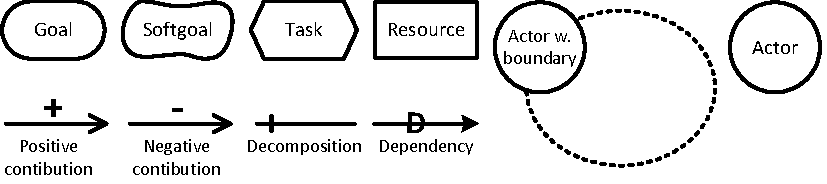
\includegraphics{img/grl_legend.pdf}
\caption{Basic elements and relationships of GRL}
\label{fig:grl_legend}
\end{figure*}


\begin{figure}[b]
\centering
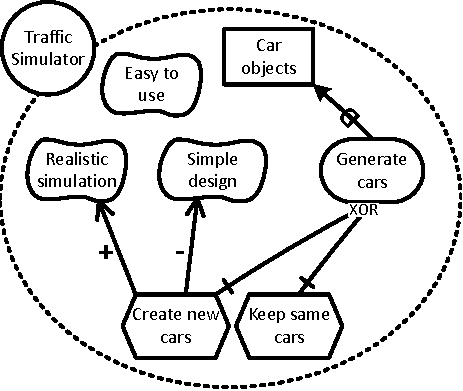
\includegraphics[width=\columnwidth]{img/Example1.pdf}
\caption{Partial GRL Model of the traffic simulator example}
\label{fig:example-small}
\end{figure} 

Figure~\ref{fig:example-small} illustrates a simplified GRL diagram from the traffic simulator design exercise. An actor represents a stakeholder of a system or the system itself (\emph{Traffic Simulator}, Figure~\ref{fig:example-small}). Actors are holders of intentions; they are the active entities in the system or its environment who want goals to be achieved, tasks to be performed, resources to be available, and softgoals to be satisfied. Softgoals differentiate themselves from goals in that there is no clear, objective measure of satisfaction for a softgoal whereas a goal is quantifiable. Softgoals (e.g. \emph{Realistic simulation}) are often related to non-functional requirements, whereas goals (such as \emph{Generate Cars}) are related to functional requirements. Tasks represent solutions to (or operationalizations of) goals and softgoals. In Figure~\ref{fig:example-small}, there are two tasks \emph{Create new cars} and \emph{Keep same cars}: in order to achieve the goal \emph{Generate cars}, the simulation can either constantly generate new ones or keep the same cars and have them reappear after they disappear off-screen. In order to be achieved or completed, softgoals, goals, and tasks may require resources to be available (e.g., \emph{Car Objects}). Finally, the full version of GRL allows design rationale to be captured using beliefs. Since we capture the reasoning and rationales behind goal models using arguments, we do not include beliefs in our simplified version of GRL (but see the discussion at the end of this section).

Different links connect the elements in a GRL model. AND, IOR (Inclusive OR), and XOR (eXclusive OR) decomposition links allow an element to be decomposed into sub-elements. In Figure~\ref{fig:example-small}, the goal \emph{Generate cars} is XOR-decomposed to the tasks \emph{Create new cars} and \emph{Keep same cars}, as they are alternative ways of achieving the goal \emph{Generate cars}. Contribution links indicate impacts of one element on another element, which can be positive or negative. Task \emph{Create new cars} has a positive contribution to the softgoal \emph{Realistic simulation}, and a negative contribution to the softgoal \emph{Simple design}. Note that the full GRL specification considers different levels of positive and negative contribution values (both quantitative and qualitative), which are not directly relevant for current purposes. Dependency links are relationships between IEs, which can model dependencies between actors. Here, the goal \emph{Generate cars} depends on the resource \emph{Car objects}. 

GRL is based on $i*$~\cite{yu1997towards} and the NFR Framework~\cite{chung2012non}, but it is less restrictive. Intentional elements and links can be more freely combined, the notion of agents is replaced with the more general notion of actors and a task does not necessarily have to be an activity performed by an actor, but may also describe properties of a solution. GRL has a well-defined syntax and semantics. Furthermore, GRL provides support for a scalable and consistent representation of multiple views/diagrams of the same goal model (see~\cite[Ch.2]{Ghanavati2013} for more details). GRL also has the capability to be extended through metadata, links, and external OCL constraints. This allows GRL to be used in many domains without the need to change the whole modeling language. For example, GRL is linked to Use Case Maps, which provides traceability between concepts and instances of the goal model and behavioral design models. Multiple views and traceability links are a good fit with our current research: we aim to add traceability links between intentional elements and their underlying arguments. 

The GRL model in Figure~\ref{fig:example-small} shows the softgoals, goals, tasks and the relationship between the different intentional elements in the model. However, the rationales and arguments behind certain intentional elements are not shown in the GRL model. Some of the questions that might be interesting to know about are the following:

\begin{itemize}
	\item Why is softgoal \emph{Easy to use} not linked to any of the goals or tasks? 
	\item What does \emph{Keep same cars} mean?
	\item Why does the task \emph{Create new cars} contribute negatively to \emph{Simple design} and positively to \emph{Realistic simulation}?
	\item Why does \emph{Generate cars} XOR-decompose into two tasks?
\end{itemize}

These are the types of the questions that we cannot answer by just looking at GRL models. The model in Figure~\ref{fig:example-small} does not contain information about discussions that led to the model, such as clarification steps for the naming, or alternatives that have been considered for the relationships. The idea behind the original GRL specification is that beliefs can be used to capture such design rationales that make later justification and review of a model easier. However, beliefs cannot be connected to links - this makes answering the third and fourth question above impossible. Furthermore, beliefs are after-the-fact design rationales and do not capture the types of questions given above. Finally, the jUCMNav tool does not consider beliefs in the evaluation algorithms, and thus there is no formal connection between goal models and their underlying beliefs and opinions. For a more detailed comparison of our framework with GRL beliefs, see Section~\ref{sect:discussions:relatedwork}. 

\subsection{Practical Reasoning Argument Scheme (PRAS)}
\label{sect:background:pras}

Reasoning about which goals to pursue and actions to take is often referred to as \emph{practical reasoning}, and has been studied extensively in philosophy and artificial intelligence. One approach is to capture practical reasoning with argument schemes~\cite{walton1990}. Applying an argument scheme results in an argument in favor of, for example, taking an action. This argument can then be tested with critical questions about, for instance, whether the action is possible given the situation, and a negative answer to such a question leads to a counterargument to the original argument for the action. 

Atkinson and Bench-Capon~\cite{atkinson2007} develop and formalize the \emph{Practical Reasoning Argument Scheme} (PRAS). A simplified version of this argument scheme is as follows:

\begin{itemize}
\item[] $G$ is a goal,
\item[] Performing action $A$ realizes goal $G$,
%\item[] Which will contribute positively to the softgoal $S$
\item[] \underline{Therefore} 
\item[] Action $A$ should be performed
\end{itemize}

Here, $G$ and $A$ are variables, which can be instantiated with concrete goals and actions to provide a specific practical argument. For example, a concrete argument about the traffic simulator is as follows: 
\begin{itemize}
\item[] \emph{Generate cars} is a goal,
\item[] Performing action \emph{Keep same cars} realizes goal \emph{Generate cars}, 
\item[] \underline{Therefore} 
\item[] Action \emph{Keep same cars} should be performed
\end{itemize}

Note that PRAS is an argument scheme that captures a full inference step: ``$G$, $A$ realizes $G$, \emph{Therefore} $A$''. There are, however, also schemes that capture simpler reasoning patterns, such as claims of the form ``$A$ does not realize $G$''. We will discuss these schemes below. 

In argumentation, conclusions which are at one point acceptable can later be rejected because of new information. For example, we may argue that, in fact, performing action \emph{Keep same cars} does not realize goal \emph{Generate cars}, thus giving a counterargument to the above instantiation of PRAS. Atkinson et al.~\cite{atkinson2007} define a set of so-called critical questions that point to typical ways in which an argument based on PRAS can be criticized. Some examples of critical questions are as follows.

\begin{enumerate}
\item[CQ1] Will the action realize the desired goal?
\item[CQ2] Are there alternative ways of realizing the same goal?
\item[CQ3] Does performing the action have a negative side effect?
\end{enumerate}

The idea is that answers to critical questions are counterarguments to the original PRAS argument. These counterarguments also follow a scheme; for example, a negative answer to CQ1 follows the scheme ``Action $A$ will not realize goal $G$'', which can be instantiated (e.g. ``\emph{Keep same cars} does not realize \emph{Generate cars''}) to form a counterargument to the original argument. 

Another way to criticize an argument for an action is to suggest an alternative action that realizes the same goal (CQ2). For example, we can argue that performing \emph{Create new cars} also realizes the goal \emph{Generate cars}. Also, it is possible that performing an action has a negative side effect (CQ3). For example, while the action \emph{Create new cars} realizes the goal \emph{Generate cars}, it has a negative side effect, namely hurting \emph{Simple design}: having the simulation constantly create new cars is fairly complex design choice. 

\begin{figure}[t]
\centering
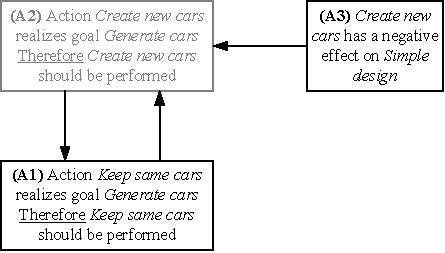
\includegraphics[]{img/fig_AF1.pdf}
\caption{PRAS arguments and attacks in the traffic simulation example.}
\label{fig:pras:example}
\end{figure}

In argumentation, counterarguments are said to \emph{attack} the original arguments. Given a set of arguments and attacks between these arguments, we can compute which arguments are accepted and which are rejected using different argumentation semantics~\cite{Dung1995}\footnote{Formal definitions of argumentation frameworks and semantics will be given in Section~\ref{sect:gmas}. In this section, we briefly discuss the intuitions behind these concepts.}. Figure \ref{fig:pras:example} shows three arguments from the traffic simulation example, where arguments are rendered as boxes and attack relations as arrows. There are two arguments based on PRAS: argument A1 for \emph{Keep Same Cars} and argument A2 for \emph{Create new cars}. Argument A2 proposes an alternative way of realizing the same goal \emph{Generate cars} with respect to argument A1 and vice versa (cf. CQ2), so A1 and A2 mutually attack each other, denoted by the arrows between A1 and A2. Argument A3 says that \emph{Create new cars} has a negative effect on \emph{Static Simulation}, so A3 attacks A2, as it points to a negative side-effect of \emph{Create new cars} (CQ3). The intuition here is that an argument is acceptable if any argument that attacks it is itself rejected. In Figure~\ref{fig:pras:example}, argument A3 is accepted because it has no attackers. This makes A2 rejected (indicated by the lighter grey color), because its attacker A3 is accepted. A1 is then also accepted, since its only attacker, A2, is rejected. 

Looking at PRAS and its critical questions, one can see how it could be used to argue about goals and actions or, more specifically, about goal models. In fact, in some of our previous work on RationalGRL \cite{vanzee-etal:renext2015,vanZee-etal:er2016} we used PRAS-arguments such as the ones above to capture reasoning about goals, and provided a translation to goal models. However, one problem of this approach is that we cannot literally use PRAS and its critical questions, as there are elements in the GRL language, such as actors and resources, which cannot be found in PRAS. Furthermore, it is not directly clear whether the critical questions as proposed by Atkinson and Bench-Capon~\cite{atkinson2007} actually apply to GRL models. In fact, our case study (Section \ref{sect:gmas}) shows that when discussing requirements, people very often do not structure their reasoning nicely in the way that PRAS presents it. That is, you do not see the discussants setting up an argument ``We have goal $G$, $A$ realizes $G$ \emph{Therefore} we should perform $A$''. A typical discussion is much more unstructured, as is clear from the transcript excerpts in Appendix~\ref{sect:transcripts:excerpts}. Thus, if we would use the version of PRAS presented in this section for our argumentation, we would violate requirement 1: The argumentation techniques must capture the actual discussions of the stakeholders or designers in the early requirements engineering phase. Our solution is to develop our own set of argument schemes and critical questions by analyzing transcripts of discussions about the traffic simulator. This set of schemes and questions and our case study are described in the next section. 


\section{Argument Schemes for Goal Modeling: a Case Study}
\label{sect:gmas}

Recall that \textbf{requirement 1} of our RationalGRL framework is that the argumentation techniques should be close to the actual discussions of stakeholders or designers in the early requirements engineering phase. To get a sense of such discussions, we performed a case study to examine which types of discourse are used during discussions of system requirements, and how these discourse types can be captured as argument schemes and critical questions. We manually coded transcripts of such discussions using a list of argument schemes and critical questions based on GRL and PRAS. In this section, we present our case study. All original transcripts, coding, and models are available in our online repository, which can be found at:  
 
\begin{quote}
\rationalgrlurl{}
\end{quote}

In order to obtain actual requirements discussions, we turned to a recent series of experiments by Tang et al. \cite{TangEtal2018}. In these experiments, 12 groups of two or three students in a Software Architecture course at MSc level were given the traffic simulator assignment (Appendix~\ref{sect:designprompt}). These groups had a maximum of two hours to design a traffic simulator, which included a discussion of the requirements of this traffic simulator. The students did not use any goal modeling technique in the course or during the discussions. They were asked to record their design sessions, and the recordings were subsequently transcribed. We used three of these transcripts, totaling 153 pages, for our case study. 


\begin{table}[t]
\centering
\begin{tabularx}{0.5\textwidth}{|l|X|l|l|l|>{\bfseries}l|}
\hline
\multicolumn{2}{|c|}{\textbf{Scheme/Question}} & $t_1$ & $t_2$ & $t_3$ & \textbf{total}\\
\hline 
AS0 & Actor & 2 & 2 & 5 & 9\\
\hline
AS1 & Resource & 2 & 4 & 5 & 11\\
\hline
AS2 & Task/action & 20 & 21 & 17 & 58\\
\hline
AS3 & Goal & 0 & 2 & 2 & 4\\
\hline
AS4 & Softgoal & 3 & 4 & 2 & 9\\
\hline
AS5 & Goal decomposes into tasks & 4 &0& 4 & 8\\
\hline
AS6 & Task contributes (negatively) to softgoal & 8 & 3 &0& 11\\
\hline
AS7 & Goal contributes (negatively) to softgoal &0& 1 & 1 & 2\\
\hline
AS8 & Resource contributes to task & 0 & 4 & 3 & 7\\
\hline
AS9 & Actor depends on actor &0& 1 & 3 & 4\\
\hline
AS10 & Task decomposes into tasks & 11 &14 &11 &36\\ 
\hline
\hline
CQ2 & Task is possible? & 2 & 2 & 1 & 5\\
\hline		
CQ5a & Does the goal decompose into the tasks? & 0 & 1 & 0 & 1\\
\hline
CQ5b & Goal decomposes into other tasks? & 1 & 0 & 0 & 1\\
\hline
CQ6b & Task has negative side effects? & 2 & 0 & 0 & 2\\
\hline
CQ10a & Task decompose into other tasks? & 1 &2 &0&3\\
\hline
CQ10b & Decomposition type correct? &1 &0& 1 &2\\
\hline
\hline
CQ11 & Is the element relevant/useful? & 2 & 3 & 2 &7\\
\hline
CQ12 & Is the element clear/unambiguous? &3 &10 & 3 & 16\\
\hline
\hline
Gen & Generic counterargument & 0& 2 & 2 & 4\\
\hline
\hline
\multicolumn{2}{|c|}{\textbf{TOTAL}}&69&80&69&222\\
\hline
\end{tabularx}
\caption{Occurrences of Argument Schemes and Critical Questions in the Transcripts.}
\label{table:transcripts:results:argumentschemes}
\end{table}

Before we started coding the transcripts, we came up with an initial list of 11 argument schemes (AS0-AS10 in Table~\ref{table:transcripts:results:argumentschemes}), representing \emph{claims} about a goal model containing the requirements of the system. We used no particular method to develop this initial list besides our own intuition about which part of a goal model would be likely to be discussed.

AS0 to AS4 are schemes that concern a single element of a goal model. For example, AS0 represents the claim `$a$ is a relevant actor for the system', and AS3 represents the claim `$G$ is a goal for the system'. AS5 to AS10 are claims about the links between GRL intentional elements. Our initial list also contained 18 critical questions, inspired by the questions associated with the original Practical Reasoning Argumentation Scheme \cite{atkinson2007}. CQ2 to CQ12 (Table~\ref{table:transcripts:results:argumentschemes}) are examples of these critical questions, other examples are `Is the softgoal legitimate?' and `Are there alternative ways to contribute to the same softgoal?'.

Using the initial list of arguments and critical questions, we coded three transcripts of requirements discussions. The coding was performed by one author and subsequently checked by other authors. As the transcripts contain spoken language, the coding involved some interpretation. For example, the students almost never literally say `actor $a$ has task $T$'. Rather, they say things such as `...we have a set of actions. Save map, open map, ...' (Table~\ref{table:transcripts:traffic-light}, Appendix~\ref{sect:transcripts:excerpts}) and `We also have to be able to change the inflow of cars. How many car come out in here on the side' (Table~\ref{table:transcript:task-clarification}, Appendix~\ref{sect:transcripts:excerpts}). Furthermore, in some cases the critical questions are explicit. For example, CQ10b is found in the transcripts as `...is this an OR or an AND?' (Table \ref{table:transcript:decomposition}, Appendix~\ref{sect:transcripts:excerpts}). In other cases, however, the question remains implicit but we added it in the coding. For example, CQ11 (`Is the element relevant/useful?') is not found directly in the transcripts, but it can be inferred from statements such as `...you don't have to specifically add a traffic light' (Table~\ref{table:transcripts:traffic-light}, Appendix~\ref{sect:transcripts:excerpts}). 

During the coding, new argument schemes and critical questions were added to the list. For example, we found that the discussants often talk about tasks decomposing into sub-tasks, therefore, we added AS10 and CQ10a. Furthermore, since there were many discussions on the relevance and the clarity of the names of elements, two generic critical questions CQ12 and CQ13 were added. The final results of the coding can be found in Table~\ref{table:transcripts:results:argumentschemes}. We found a total of 159 instantiations of argument schemes AS0-AS10. The most used argument scheme was AS2: ``Actor $A$ has task $T$'', however, each argument scheme is found in transcripts at least twice. A large portion (about 60\%) of argument schemes involved discussions about tasks of the information system (AS2, AS10). We coded 41 applications of critical questions. Many critical questions (about 55\%) involved clarifying the name of an element, or discussing its relevance (CQ12, Gen).

Our coding further led us to identify three different operations, that represent different effects an argument or critical question can have on a goal model: an argument can introduce a new element in the goal model (\textsf{INTRO}); it can disable (i.e. attack) a goal model element (\textsf{DISABLE}); or it can replace an element in the goal model with another one (\textsf{REPLACE}). Consider, for example, Table~\ref{table:transcripts:traffic-light} in Appendix~\ref{sect:transcripts:excerpts}. First, an argument is posed that introduces a number of tasks. A counterargument is then given against one of these tasks (\emph{add traffic light}), which is subsequently disabled. An example of replacement is given in Table~\ref{table:transcript:decomposition} (Appendix~\ref{sect:transcripts:excerpts}): what used to be an AND-decomposition is changed into an OR-decomposition. We will further discuss these operations in Section~\ref{sect:overview} with various examples, and we formalize the operations in Section~\ref{sect:formalframework} with algorithms.
\section{The RationalGRL Framework}
\label{sect:overview}

We now turn to an overview of our RationalGRL framework. We will show through a metamodel and informal examples from our case study that it is possible to trace elements of the goal model back to their underlying arguments (\textbf{requirement 2}), and that it is possible to determine the effect of changes in the underlying argumentation on the goal model, and vice versa (\textbf{requirement 3}). A formalization of our framework using formal logic can be found in Section~\ref{sect:formalframework}.

Figure~\ref{fig:rationalgrl-framework} presents an overview of the RationalGRL framework. There are two activities (bottom), \emph{Practical reasoning \& argumentation} and \emph{Goal model construction}, which give rise to two different models (top), a \emph{RationalGRL model} and a \emph{GRL model}. The GRL part of RationalGRL allows for the creation of goal models by analyzing the non-functional requirements and refining the high-level goals into operationalized tasks. For the argumentation part, arguments and counterarguments can be put forward about various parts of this goal model. These two parts, GRL and argumentation, can impact the other side so that the models can be refined or new critical questions and argument schemes can be instantiated. For example, answering a critical question \emph{Is the task \emph{A} possible?} can result in removing or adding a task in the GRL model. Similarly, if, for example, we add a new intentional element to the GRL model, it can lead to a new critical question relevant to this intentional element and its relationships. Thus, in the framework it is possible to trace a goal model back to the original discussions about goals, tasks and requirements. 

\begin{figure}[t]
\centering
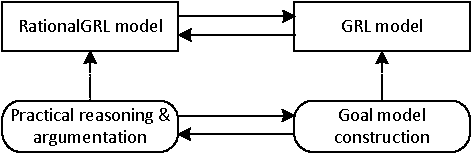
\includegraphics[width=\columnwidth]{img/framework.pdf}
\caption{The RationalGRL Framework}
\label{fig:rationalgrl-framework}
\end{figure}

\begin{table*}[t]
\centering
\begin{tabularx}{\textwidth}{|l|l|l|X|l|}
\hline
\multicolumn{2}{|c|}{\textbf{Argument scheme}} & \multicolumn{2}{c|}{\textbf{Critical Questions}} & \textbf{Effect}\\
\hline
AS0 & $a$ is an actor & CQ0 & Is the actor relevant? & \textsf{DISABLE} (no)\\
\hline
AS1 & Actor $a$ has resource $R$ & CQ1 &Is the resource available? & \textsf{DISABLE} (no)\\
\hline
AS2 & Actor $a$ can perform task $T$ & CQ2a &Is the task possible? & \textsf{DISABLE} (no)\\
&& CQ2b & Does the task have negative side-effects? & \textsf{DISABLE} (yes)\\
\hline
AS3 & Actor $a$ has goal $G$ & CQ3 & Can the desired goal be realized? & \textsf{DISABLE} (no)\\
\hline
AS4 & Actor $a$ has softgoal $S$ & CQ4 & Is the softgoal a legitimate softgoal?& \textsf{DISABLE} (no)\\
\hline
\hline
AS5 & Goal $G$ decomposes into task $T$ & CQ5a & Does the goal decompose into the task?& \textsf{DISABLE} (no)\\
& & CQ5b & Does the goal decompose into other tasks? & \textsf{INTRO} (yes)\\
 &  & CQ5c & Is the decomposition type correct? & \textsf{REPLACE} (no)\\
\hline
AS6 & Task $T$ contributes (negatively) to softgoal $S$& CQ6a & Does the task contribute to the softgoal?& \textsf{DISABLE} (no)\\
&& CQ6b & Are there alternative ways of contributing to the same softgoal?& \textsf{INTRO} (yes) \\
&& CQ6c & Does the task contribute (negatively) to some other softgoal?& \textsf{INTRO} (yes)\\
\hline
AS7 & Goal $G$ contributes to softgoal $S$ & CQ7a & Does the goal contribute to the softgoal?& \textsf{DISABLE} (no)\\
&& CQ7b & Does the goal contribute to some other softgoal?& \textsf{INTRO} (yes)\\
\hline
AS8 & Task $T$ depends on resource $R$ & CQ8 & Is the resource required in order to perform the task?& \textsf{DISABLE} (no)\\
\hline
AS9 & Actor $a$ depends on actor $b$ & CQ9 & Does the actor depend on any actors?& \textsf{INTRO} (yes)\\
\hline
AS10 & Task $T_i$ decomposes into task $T_j$ & CQ10a & Does the task decompose into the task? & \textsf{DISABLE} (no)\\
 &  & CQ10b & Does the task decompose into other tasks?& \textsf{INTRO} (yes)\\
 &  & CQ10c & Is the decomposition type correct? & \textsf{REPLACE} (no)\\
\hline
AS11 & Element $IE$ is relevant & CQ11 & Is the element relevant/useful? & \textsf{DISABLE} (no)\\
\hline
AS12 & Element $IE$ has name $n$ & CQ12 & Is the name clear/unambiguous? & \textsf{REPLACE} (no)\\
\hline
\hline
Att & Generic counterargument & Att & Generic counterargument & \textsf{DISABLE}\\
\hline
\end{tabularx}
\caption{List of argument schemes (AS0-AS13), critical questions (CQ0-CQ12), and the effect of answering them (right column).}
\label{table:argument-schemes}
\end{table*}

In the rest of this section we discuss the individual parts of the GRL framework. In Section~\ref{sect:overview:as}, we continue our discussion of the argument schemes and critical questions for practical reasoning and argumentation, fitting these schemes and questions into our framework. In Section~\ref{sect:overview:lang}, we then discuss the language for RationalGRL models an we provide a metamodel, linking the new concepts of our language to GRL. In Section~\ref{sect:overview:examples}, we provide extensive examples from our case study.  

\subsection{The RationalGRL Argument Schemes and Critical Questions for Practical Reasoning}
\label{sect:overview:as}

A core aspect of the RationalGRL framework are the argument schemes, which should be close to the actual discussions of stakeholders (\textbf{requirement 1}). Recall from Section \ref{sect:gmas} that we ended up with a list of argument schemes and critical questions that were found in the transcripts (Table~\ref{table:transcripts:results:argumentschemes}). Using this list as a basis, we further refined the set of argument schemes and critical questions for RationalGRL into the list shown in Table~\ref{table:argument-schemes}. 

It is important to note that the list we provide here is not exhaustive. It is merely the result of our empirical study, but new new argument schemes and questions can be added depending on the problem domain. In fact, our tool (Section~\ref{sect:tool}) contains many more critical questions, and it is fully extensible, meaning that new argument schemes and critical questions can be added easily. See Section~\ref{sect:discussion:futurework} for more details.

Schemes AS0-AS4 and AS11-AS12 are arguments for an element of a goal model, and AS5-AS10 are related to links in a goal model. The last scheme (Att) is a scheme for a generic counterargument against any type of argument that has been put forward. Arguments based on the schemes in Table~\ref{table:argument-schemes} can be used to form arguments about elements in a GRL model. Making an argument based on one of the schemes effectively adds the corresponding GRL element to the model. See, for example, Table~\ref{table:transcripts:traffic-light} in Appendix~\ref{sect:transcripts:excerpts}: the participants argue for the addition of several tasks to the goal model using argument scheme AS2. 

An important part of arguing about goal models is asking the right critical questions. The critical questions presented in Table~\ref{table:argument-schemes} are therefore related to their respective argument schemes. These questions can be answered with ``yes'' or ``no'', and the type of answer has an effect on the original argument (\textsf{INTRO}, \textsf{DISABLE}, \textsf{REPLACE}). This will be further explained in Section~\ref{sect:overview:examples} an in Section~\ref{sect:formalframework}.


\subsection{The RationalGRL Modeling Language}
\label{sect:overview:lang}
\label{sect:metamodel}
RationalGRL is an extension of GRL and includes all the elements shown in Figure~\ref{fig:grl_legend}. However, there are also new elements corresponding to argumentation-related concepts. Figure~\ref{fig:rationalgrllegend} shows these elements. 
\begin{itemize}
\item \emph{Argument}: This represents an argument that does not directly correspond to a GRL element.  
\item \emph{Rejected (Disabled) GRL element}: If an argument or GRL element is attacked by an argument that itself is not attacked, then this GRL element will be rejected. Note Figure~\ref{fig:rationalgrllegend} only shows one type of disabled element, a Task, but all the elements (IEs and links) can be disabled in RationalGRL.
\item \emph{Attack Link}: An attack link can occur between an argument and another argument or GRL element. It means that the source argument attacks the target argument or GRL element.
\end{itemize} 

\begin{figure}[b]
\centering

\includegraphics{img/legend.pdf}
\caption{The new elements and link of RationalGRL. Generic argument (left), attack link (middle), and disabled element (right). The disabled element in this figure is a task, but all IEs and links can be disabled in RationalGRL}
\label{fig:rationalgrllegend}
\end{figure}


The complete metamodel of the language can be found in Figure~\ref{fig:metamodel}. This metamodel represents the abstract grammar of the language, independently of the notation. The metamodel also formalizes the GRL concepts and constructs introduced in Section~\ref{sect:background:grl}.

\begin{figure*}[t]
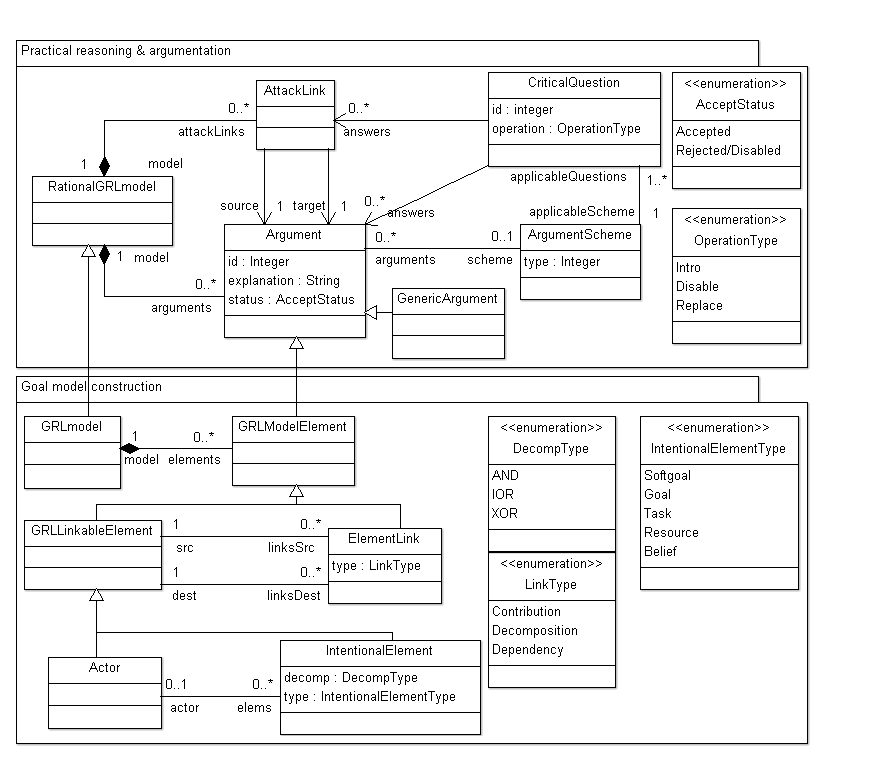
\includegraphics[width=\textwidth]{metamodel/metamodel}
\caption{The RationalGRL metamodel. The \emph{Goal model construction} package (bottom) is the GRL metamodel. The \emph{Practical reasoning \& argumentation} package is the RationalGRL extension}
\label{fig:metamodel}
\end{figure*}

The metamodel consists of two packages, \emph{Practical reasoning \& argumentation} and \emph{Goal model construction}, which correspond to the relevant activities in the RationalGRL framework (cf. Figure~\ref{fig:rationalgrl-framework}). The goal model construction package is simply the GRL metamodel. It consists of \textsf{GRLModelElements}, which can be either \textsf{GRLLinkableElements} or \textsf{ElementLinks}. A \textsf{GRLLinkableElement} can again be specialized into an \textsf{Actor} or an \textsf{IntentionalElement} (which is either a \textsf{Softgoal}, \textsf{Goal}, \textsf{Task}, \textsf{Resource}, or a \textsf{Belief}). Intentional elements can be part of an actor, and \textsf{GRLLinkableElements} are connected through \textsf{ElementLinks} of different types (i.e., \textsf{Contribution, Decomposition}, or \textsf{Dependency}). Finally, a \textsf{GRLmodel} is composed of \textsf{GRLModelElements}.

The practical reasoning and argumentation package depicts the concepts we introduced in Section~\ref{sect:overview:as}. An \textsf{ArgumentScheme} represents a scheme containing variables. \textsf{CriticalQuestions} are possible ways to attack or elaborate an argument based on a scheme; each critical question applies to exactly one scheme, but for each scheme there may be more than one applicable critical question. When an argument scheme is instantiated, we obtain an \textsf{Argument}. Therefore, each argument is associated with exactly one scheme, but a scheme can be instantiated in multiple ways. When a critical question is answered, we may obtain an \textsf{AttackLink}, an \textsf{Argument} or both, depending on the answer. Note that it is also possible for an \textsf{AttackLink} to be associated with no critical questions. This allows the user to create attacks between arguments, which do not necessarily correspond to one of the critical questions. A \textsf{RationalGRLmodel} is composed out of arguments and attack relations.

The \textsf{OperationTypes} in the Argumentation package correspond to the operations we informally introduced in Section~\ref{sect:overview}. These operations are performed by instantiating an argument scheme or answering a critical question in a certain way. An \textsf{INTRO} operation introduces a new RationalGRL element. A \textsf{DISABLE} operation creates a new argument that attacks another argument or GRL element, effectively disabling it. The \textsf{REPLACE} operation replaces a RationalGRL element with a new element. Instantiating an argument scheme from Table~\ref{table:argument-schemes} always leads to an \textsf{INTRO} operation, that is, it always introduces a new RationalGRL element. Answering a critical question can have different effects depending on the critical question and the answer. Table~\ref{table:argument-schemes} shows these effects for the different critical questions and answers. For example, answering CQ0 with ``no'' disables the argument based on AS0. 

There are two important links between the \emph{practical reasoning \& argumentation} and \emph{goal model construction} packages. First, each \textsf{GRLModelElement} is an \textsf{Argument}. This means that each model element inherits the \textsf{AcceptStatus} as well, allowing GRL elements to be accepted or rejected. This, furthermore, means that argument schemes can be applied to all GRL elements, capturing the intuition that each GRL element can be regarded as an instantiated argument scheme. Note that besides arguments about elements of the GRL model, we also have a \textsf{GenericArgument} which is simply a counter-argument to an existing argument that does not relate to any of the GRL elements. Finally, the relation between \textsf{GRLModelElement} and \textsf{Argument} means that, as we already briefly indicated when discussing the framework in Figure~\ref{fig:rationalgrl-framework}, the class of \textsf{RationalGRLmodel} is a superclass of \textsf{GRLmodel}: besides arguments about GRL elements, we can also have arguments that does not relate to any of the GRL elements.

\subsection{From Practical Reasoning to RationalGRL Models: examples from the case study}
\label{sect:overview:examples}

We now turn to the interactions between the \emph{practical reasoning \& argumentation} (i.e. the bottom left element of the framework in Figure~\ref{fig:rationalgrl-framework}) on the one hand, and \emph{RationalGRL models} (i.e. the top left element of the framework in Figure~\ref{fig:rationalgrl-framework}) on the other hand. We provide informal examples of the links between the practical reasoning found in our case study transcripts and RationalGRL models. The formal grounding for the connection between practical reasoning and RationalGRL models can be found in the RationalGRL metamodel (Section~\ref{sect:metamodel}) and in more detail in the logical formalization in the next section. The connection between the RationalGRL models shown in this section and regular GRL models is further formally defined in Section \ref{sect:formalframework:translation}. 

\paragraph{Example 1 - Introducing GRL elements with arguments (\textsf{INTRO)}}

\begin{figure}[t]
\centering
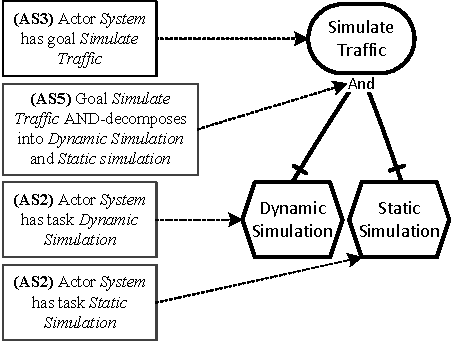
\includegraphics[width=\columnwidth]{img/fig_example_AS.pdf}
\caption{RationalGRL model (right) with instantiated argument schemes (left): Introducing new elements (operation \textsf{INTRO)}}. 
\label{fig:example_AS}
\end{figure}

We start by showing how instantiating argument schemes leads to the introduction of new RationalGRL elements in a model. Take the example in Figure~\ref{fig:example_AS}, which is based on the excerpt from transcript $t_3$ shown in Table~\ref{table:transcript:decomposition} in Appendix~\ref{sect:transcripts:excerpts}. On the left side of the image, the arguments found in the transcript are shown, together with the argument scheme they are based on. The participants in the discussion argue that actor \emph{System} has a goal and two tasks, and that the goal AND-decomposes into the two tasks. By putting forward these arguments, new GRL elements are introduced. These GRL elements are shown on the right side of Figure~\ref{fig:example_AS}; the dashed arrows indicate the links between the practical reasoning and argumentation on the left and the RationalGRL model on the right.


\paragraph{Example 2: Disabling GRL elements by answering critical questions (\textsf{DISABLE)}}

\begin{figure}[b]
\centering
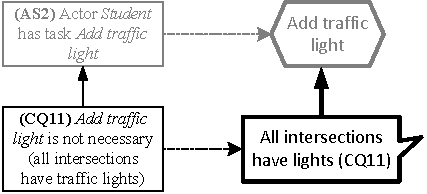
\includegraphics[]{img/fig_example_disable.pdf}
\caption{Disabling elements (operation \textsf{DISABLE)}.}
\label{fig:example_disable}
\end{figure}

The excerpt from transcript $t_1$ used in this example is shown in Table~\ref{table:transcripts:traffic-light} in Appendix~\ref{sect:transcripts:excerpts}. In this example, participants first sum up functionality of the traffic simulator, which can be captured as instantiations of AS2. On left side of Figure~\ref{fig:example_disable} one such instantiation is shown, which leads to the addition of the task \emph{Add traffic light} in the RationalGRL model on the right side of Figure~\ref{fig:example_disable}. However, participant P1 notes that the problem description states that all intersections have traffic lights by default, so the task \emph{Add traffic light} is not necessary. This is captured using critical question CQ11. A negative answer to this question (cf. Table~\ref{table:argument-schemes}) should disable the original argument based on AS2 by attacking it. On the left side of Figure~\ref{fig:example_disable} a new argument (CQ11) attacks the original argument based on argument scheme AS2. This new argument is also added to the RationalGRL model on the right of Figure~\ref{fig:example_disable}, where it attacks the original task \emph{Add traffic light}. This attack leads to the original argument being \emph{rejected} (cf. Section~\ref{sect:background:pras} and Section~\ref{sect:formalframework:rationalgrl}), indicated by it being greyed out. As a result of this, the corresponding GRL task \emph{Add traffic light} is also disabled. 

\paragraph{Example 3: Changing a decomposition type by answering critical questions (\textsf{REPLACE})} 

\begin{figure}[t]
\centering
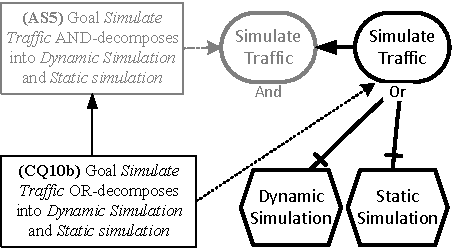
\includegraphics[]{img/fig_example_replace.pdf}
\caption{Replacing an element (operation \textsf{REPLACE)}.}
\label{fig:examples:decomposition}
\end{figure}

The excerpt of transcript $t_3$ used for this example is shown in Table~\ref{table:transcript:decomposition} in Appendix~\ref{sect:transcripts:excerpts}. It consists of a discussion about the type of decomposition relationship for the goal \emph{Simulate Traffic} (Figure~\ref{fig:examples:decomposition}). Recall that in Example 1, an AND-decomposition was introduced for this goal with AS5 (Figure~\ref{fig:example_AS}). In the discussion CQ5c -- ``Is the decomposition type correct?'' -- is explicitly asked. The answer is ``No, it should be OR''. The original argument for AND-decomposition is now attacked  by the argument for the OR-decomposition, and the new argument is linked to the OR-decomposition in the RationalGRL model. 

\begin{figure}[b]
\centering
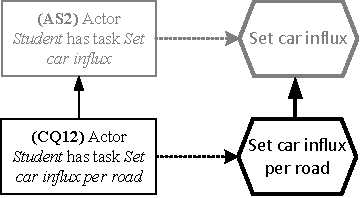
\includegraphics[]{img/fig_example_rename.pdf}
\caption{Renaming an element name (operation \textsf{REPLACE)}.}
\label{fig:examples:clarification}
\end{figure}

\paragraph{Example 4: Clarifying a task by answering critical questions (\textsf{REPLACE})}

The transcript excerpt of this example is shown in Table~\ref{table:transcript:task-clarification} in Appendix~\ref{sect:transcripts:excerpts} and comes from transcript $t_1$. The discussion starts with an instantiation of argument scheme AS2: ``Actor \emph{Student} has task \emph{Set car influx}'' (Figure~\ref{fig:examples:clarification}). This argument is then challenged with critical question CQ12: ``Is the task \emph{Set car influx} specific enough?''. This is answered negatively, creating a new argument ``Actor \emph{Student} has task \emph{Set car influx per road}'', which attacks the original argument for \emph{Set car influx}. Note how the new task \emph{Set car influx per road} also attacks (and disables) the original RationalGRL task \emph{Set car influx}. 


\paragraph{Example 5: Defending the addition of an actor (\textsf{DISABLE)}}

\begin{figure}[t]
\centering
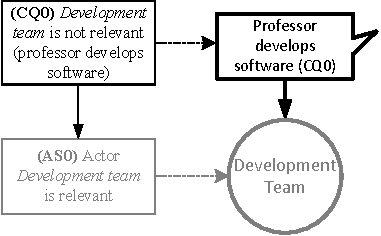
\includegraphics[]{img/reinstate1.pdf}
\caption{Disabling an element (operation \textsf{DISABLE)}.}
\label{fig:examples:relevant-actor}
\end{figure}

The excerpt from transcript $t_3$ used in this example is shown in Table~\ref{table:transcript:irrelevant-actor} in Appendix~\ref{sect:transcripts:excerpts}. Actor \emph{Development Team} is introduced with an argument based on AS0 (Figure~\ref{fig:examples:relevant-actor}). This is then attacked by arguing that the professor will develop the software, so there will not be any development team (CQ0). 

\begin{figure}[b]
\centering
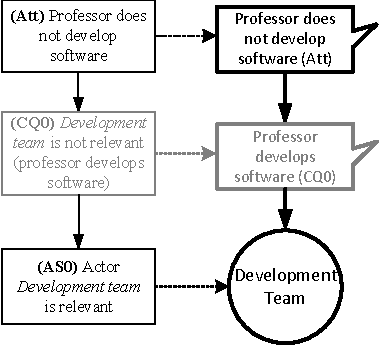
\includegraphics[]{img/reinstate2.pdf}
\caption{Defending an element by attacking its disabling attacker (operation \textsf{DISABLE)}.}
\label{fig:examples:relevant-actor2}
\end{figure}

Further in the discussion, it is then argued that the development team should be considered, since the professor does not develop the software. This is captured using a generic counterargument \emph{Att}, which attacks the earlier argument based on CQ0. Figure~\ref{fig:examples:relevant-actor2} shows the situation after the counterargument has been put forward: the argument (Att) now attacks the argument (CQ0), which in turn attacks the original argument (AS0). As a result, the argument (AS0) is acceptable (cf. Section~\ref{sect:background:pras} and Section~\ref{sect:formalframework:rationalgrl}), which causes the actor in the RationalGRL model to be enabled again.


%\section{Examples from the Transcripts}
\label{sect:examples}

In the previous section we discussed the results of our empirical analysis, and we used a simplified version of one of the transcripts as a motivating example. In this section, we provide examples from all of the three transcripts in more detail. Note that the examples in this section do not always come from Figure~\ref{fig:transcripts:grl}, but they may come from any of the three transcripts.

For each example, we provide transcript excerpts, a visualization of arguments, and the corresponding goal model elements. As we explained in the previous section, Figure~\ref{fig:transcripts:grl} shows an example of how a RationalGRL model may look like when it is developed in our prototype tool. However, the argument schemes that are instantiated are left implicit in this figure (in the tool, they can be seen in the details pane, see Section~\ref{sect:tool}). Since we would like to make these instantiated argument schemes explicit in the examples below, we use a different visual language here. We provide a legend for our visualization notation in Figure~\ref{fig:legend}.

\begin{figure}[ht!]
\centering
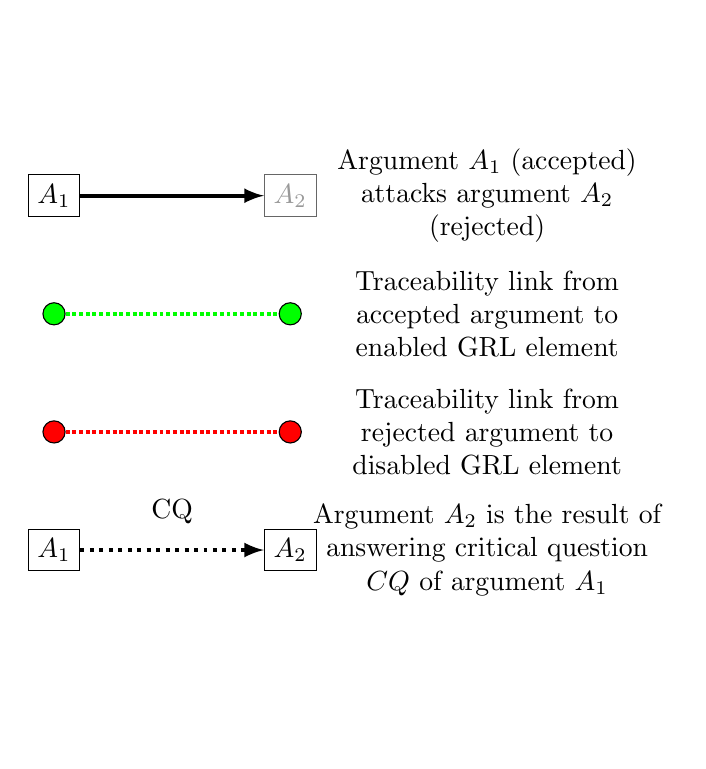
\begin{tikzpicture}
        \node (att1) [argNodeIN] at (-5,0) {$A_1$};
        \node (att2) [argNodeOUT] at (-2,0) {$A_2$};
        \node (attDescription) [draw=none, align=center] at (0.5,0) {Argument $A_1$ (accepted)\\ attacks argument $A_2$\\ (rejected)};
        \node[traceNodeGREEN] (trace1a) at (-5,-1.5) {};
        \node[traceNodeGREEN] (trace1b) at (-2,-1.5) {};
        \node (traceDescription) [draw=none,align=center] at (0.5,-1.5) {Traceability link from\\ accepted argument to\\ enabled GRL element};
        \node[traceNodeRED] (trace2a) at (-5,-3) {};
        \node[traceNodeRED] (trace2b) at (-2,-3) {};
        \node (traceDescription) [draw=none,align=center] at (0.5,-3) {Traceability link from\\ rejected argument to\\ disabled GRL element};
        \node (cq1) [argNodeIN] at (-5,-4.5) {$A_1$};
        \node (cq2) [argNodeIN] at (-2,-4.5) {$A_2$};
        \node (cqDescription) [draw=none,align=center] at (0.5,-4.5) {Argument $A_2$ is the result of\\ answering critical question\\ $CQ$ of argument $A_1$};
         \path
    (att1) edge [attackLink] (att2)
    (cq1) edge [CQLink] node [above,draw=none] {CQ} (cq2)
    (trace1a) edge[traceLinkGREEN] (trace1b)
    (trace2a) edge[traceLinkRED] (trace2b);
\end{tikzpicture}
\caption{Legends of Various Elements and Relationships}
\label{fig:legend}
\end{figure}

\subsubsection{Example 1: Methodology example}

In this section, we present a small example for the RationalGRL methodology. This example is based on the traffic simulator example described in Section~\ref{sect:goals:runningexample}. We base argument schemes and critical questions of this example on a transcript containing discussions about the development of this traffic simulator system. %These transcripts are created as part of two master theses on improving design reasoning~\cite{masterthesis1,masterthesis2}. %TODO again?
%We provide several more examples in Section~\ref{sect:examples}.

As mentioned in Section~\ref{sect:goals:runningexample}, a group of stakeholders are developing a goal model for a traffic simulator example and they are modeling the goal \texttt{Simulate Traffic} using the RationalGRL methodology. This proceeds in the following way:
\begin{itemize}
\item
First they start %at step \emph{Modify GRL models} (Figure~\ref{fig:rationalgrl-methodology}), 
with the initial GRL model (Figure~\ref{fig:example-small}) and they invoke the intentional element \texttt{Simulate Traffic}. 
\item Next, they switch to the argumentation part (step \emph{Instantiate arguments schemes}). They answer critical question \emph{Does Simulate Traffic AND-decompose into any tasks?} with \emph{Yes: namely tasks ``Dynamic Simulation'' and ``Static Simulation"}.
\item As a result, two argument schemes are created, namely:
\begin{itemize}
\item Actor \texttt{Traffic Simulator} has task \texttt{Dynamic Simulation}
\item Actor \texttt{Traffic Simulator} has task \texttt{Static Simulation}
\end{itemize}
\item In the GRL model, this corresponds to the addition of two tasks, and an AND-decomposition from the goal \emph{Simulate Traffic} to these two tasks.
\item Next, the stakeholders test the validity of their goal model by answering more critical question. They answer two critical questions:
\begin{itemize}
\item
CQ \emph{Is task ``Dynamic Simulation'' relevant} is answered with ``No, it is not relevant since the problem specification explicitly states dynamic simulations are not required''. Thus, the corresponding GRL intentional element is disabled.
\item The decomposition is changed from AND to OR, since it turned out not both tasks can be implemented together.
\end{itemize}
\end{itemize}

An excerpt of the RationalGRL model is shown in Figure~\ref{fig:examples:decomposition}. %TODO You need to update goal "simulate" in this figure to "Simulate Traffic".  Also, I don't think we should really call it the rational GRL model. it is an excerpts of the model. 


\subsubsection{Example 2: Disable task \texttt{Traffic light}}

The transcript excerpt of this example is shown in Table~\ref{table:transcripts:traffic-light} in the appendix and comes from transcript $t_1$. In this example, participants sum up functionality of the traffic simulator, which are tasks that the students can perform in the simulator. All these tasks can be formalized and are instantiated from  argument scheme AS2: ``Actor \emph{Student} has tasks $T$'', where $T\in\{$Save map, Open map, Add intersection, Remove intersection, Add road, Add traffic light$\}$''. 

Once all these tasks are summed up, participant \texttt{P1} notes that the problem description states that all intersections in the traffic simulator have traffic lights, so the task \texttt{Add traffic light} is not necessary. We formalized this using the critical question CQ12: ``Is task \texttt{Add traffic light} useful/relevant?''. %TODO I think it is better to say "necessary" and "not necessary" --> change figure 8: useless --> not necessary

We visualize some of the argument schemes, critical questions, and traceability links with GRL model in Figure~\ref{fig:examples:traffic-light}. On the left side of the image, we see three of the instantiated argument schemes AS2. The bottom one, ``Actor \texttt{Student} has task \texttt{Add traffic light}'', is attacked by another argument generated from applying critical question CQ12: ``\texttt{Add traffic light} is %useless 
not necessary (\emph{All intersections have traffic lights})''. As a result, the corresponding GRL task is disabled. The other two tasks are enabled and have green traceability links.

\begin{figure}[ht!]
\centering
        \begin{tikzpicture}
        \node (a0) [argNodeIN] at (-2,0) {
        	\argtext{AS2}{Actor \emph{Student} has task \emph{Save map}}
        };
        \node (a1) [argNodeIN] at (-2,-2) {
        	\argtext{AS2}{Actor \emph{Student} has task \emph{Add road}}
        };
        \node (a2) [argNodeOUT] at (-2,-4) {
        	\argtext{AS2}{Actor \emph{Student} has task \emph{Add traffic light}}
        };
        \node (a3) [argNodeIN] at (-2,-6){
        	\argtext{}{\emph{Add traffic light} is not necessary (\emph{All intersections have traffic lights})}
        };
        \node[grl] (task1) at (2.3,0) { \includegraphics[scale=0.5]{img/task_save_map} };
        \node[grl] (task2) at (2.3,-2) { \includegraphics[scale=0.5]{img/task_add_road} };
        \node[grl, disabled] (task3) at (2.3,-4) { \includegraphics[scale=0.5]{img/task_add_traffic_light} };
        \node[traceNodeGREEN] (trace1a) at (-.4,-.3) {};
        \node[traceNodeGREEN] (trace1b) at (2.2,-.3) {};
        \node[traceNodeGREEN] (trace2a) at (-.4,-2.3) {};
        \node[traceNodeGREEN] (trace2b) at (2.2,-2.3) {};
        \node[traceNodeRED] (trace3a) at (-.4,-4.3) {};
        \node[traceNodeRED] (trace3b) at (2.2,-4.3) {};
         \path
    (a3) edge [attackLink] (a2)
    (a2) edge [CQLink, bend right=50] node [left,draw=none] {CQ12} (a3)
    (trace1a) edge[traceLinkGREEN] (trace1b)
    (trace2a) edge[traceLinkGREEN] (trace2b)
    (trace3a) edge[traceLinkRED] (trace3b);
\end{tikzpicture}
\caption{Argument Schemes and Critical Questions (left), GRL Model (right), and Traceability Link (dotted lines) for the Traffic Light Example.}
\label{fig:examples:traffic-light}
\end{figure}


\subsubsection{Example 3: Clarify task \texttt{Road pattern}}

The transcript excerpt of the second example is shown in Table~\ref{table:transcript:task-clarification} in Appendix~\ref{sect:transcripts:excerpts} and comes from transcript $t_3$. It consists of a number of clarification steps, resulting in the task \texttt{Choose a road pattern}. 
%TODO where is this task in the model?
%MvZ: It is in Figure 9, but not in Figure 6. Figure 6 is just a single model from our transcripts, but Figure 9 comes from another transcript. Do you think it is better to take all of the examples from the same transcript? I feel that may look a bit strange since we are completely disregarding the other transcripts then.

\begin{figure}[ht!]
\centering
        \begin{tikzpicture}[->]
        \node (a0) [argNodeOUT] at (-2,0) {
        	\argtext{AS2}{Actor \emph{Student} has task \emph{Create road}}
        };
        \node (a1) [argNodeOUT] at (-2,-2) {
        	\argtext{AS2}{Actor \emph{Student} has task \emph{Choose a pattern}}
        };
        \node (a2) [argNodeOUT] at (-2,-4.2) {
        	\argtext{AS2}{Actor \emph{Student} has task \emph{Choose a pattern preference}}
        };
        \node (a3) [argNodeIN] at (-2,-6.7) {
        	\argtext{AS2}{Actor \emph{Student} has task \emph{Choose a road pattern}}
        };
        \node[grl] (actor) at (2.3,-4) { 
        	\includegraphics[scale=0.5]{img/task_choose_road_pattern} 
        };
        \node[traceNodeGREEN] (trace1) at (-.5,-7.1) {};
        \node[traceNodeGREEN] (trace2) at (2.2,-4.4) {};

\begin{pgfonlayer}{background}
         \path
    (a1) edge[attackLink] (a0)
    (a2) edge[attackLink] (a1)
    (a2) edge[attackLink, bend right=20] (a0)
    (a3) edge[attackLink] (a2)
    (a3) edge[attackLink, bend right=20] (a1)
    (a3) edge[attackLink, bend right=40] (a0);
\end{pgfonlayer}

	\path
	(a0) edge [CQLink, bend right=50] node [left,draw=none] {CQ12a} (a1)
    (a1) edge [CQLink, bend right=50] node [left,draw=none] {CQ12a} (a2)
    (a2) edge [CQLink, bend right=50] node [left,draw=none] {CQ12a} (a3)
    (trace1) edge[traceLinkGREEN] (trace2);
\end{tikzpicture}
\caption{Argument Schemes and Critical Questions (left), GRL Model (right), and Traceability Link (dotted line) for the Road Pattern Example.}
\label{fig:examples:clarification}
\end{figure}

The formalized argument schemes and critical questions are shown in Figure~\ref{fig:examples:clarification}. The discussion starts with the first instantiation of argument scheme AS2: ``Actor \texttt{Student} has task \texttt{Create road}''. 
%TODO I don't see it in Figure 6.
%MvZ: see previous comment, Figure 9 is not part of Figure 6
This argument is then challenged with critical question CQ12: ``Is the task \texttt{Create road} clear?''. Answering this question results in a new instantiation of argument scheme AS2: ``Actor \texttt{Student} has task \texttt{Choose a pattern}''. %TODO same %MvZ same
This process is repeated two more times, resulting in the final argument ``Actor \texttt{Student} has task \texttt{Choose a road pattern}''. This final argument is "un-attacked" and has a corresponding intentional element (right image). 

What is clearly shown in this example is that a clarifying argument attacks all arguments previously used to describe the element. For instance, the final argument on the bottom of Figure~\ref{fig:examples:clarification} attacks all three other arguments for a name of the element. If this is not the case, then it may occur that a previous argument is \emph{re-instantiated}, meaning that it becomes accepted again because the argument attacking it, is itself attacked. Suppose for instance that the bottom argument ``Actor \texttt{Student} has task \texttt{Choose a pattern preference}'' did not attack the second argument: ``Action \texttt{Student} has task \texttt{Choose a pattern}''. In that case, this argument would be re-instantiated, because its only attacker ``Actor \texttt{Student} has task \texttt{Choose a pattern preference}'' is itself defeated by the bottom argument. %TODO check these tasks with the GRL model of Figure 6. Also, I recommend to have the changed full  GRL model after we finish the examples to show how the model improves. 

\subsubsection{Example 4: Decompose goal \texttt{Simulate}} %TODO In fig 1, the goal is called simulate traffic which makes more sense. goal "simulate" is a bit meaningless. I suggest to update fig 6 and all the other ones accordingly. Also, we are refering to this example in example 1. Why can't we merge them?

\todo{Marc}{all}{Check whether the text matches the figure here}
The transcript excerpt of this example is shown in Table~\ref{table:transcript:decomposition} in the appendix and comes from transcript $t_3$. It consists of a discussion about the type of decomposition relationship for the goal \texttt{Simulate}.

\begin{figure}[ht]
\begin{adjustwidth}{-3em}{}
        \begin{tikzpicture}[->]
        \node (a0) [argNodeIN] at (-2,0.5) {
        	\argtext{CQ3}{Task \emph{Dynamic simulation} is not relevant}
        };
        \node (a1) [argNodeIN] at (-2,-1.5) {
        	\argtext{AS2}{Actor \emph{System} has task \emph{Dynamic simulation}}
        };
        \node (a2) [argNodeIN] at (-2,-3) {
        	\argtext{AS2}{Actor \emph{System} has task \emph{Static simulation}}
        };
        \node (a3) [argNodeOUT] at (-2,-4.5) {
        	\argtext{AS5}{Goal \emph{Simulate} AND-decomposes into \emph{Static simulation} and \emph{Dynamic simulation}}
        };
        \node (a4) [argNodeIN] at (-2,-7.5) {
        	\argtext{AS5}{Goal \emph{Simulate} OR-decomposes into \emph{Static simulation} and \emph{Dynamic simulation}}
        };
        \node[grl] (actor) at (2.2,-4) { 
        	\includegraphics[scale=0.5]{img/simulate_decomposition} 
        };
        \node[traceNodeRED] (trace2a) at (-.4,-1.8) {};
        \node[traceNodeRED] (trace2b) at (3.2,-5.6) {};
        \node[traceNodeGREEN] (trace3a) at (-.4,-3.3) {};
        \node[traceNodeGREEN] (trace3b) at (1,-5.6) {};
        \node[traceNodeGREEN] (trace4a) at (-.4,-8.2) {};
        \node[traceNodeGREEN] (trace4b) at (2.2,-3.9) {};

\begin{pgfonlayer}{background}
         \path
    (a1) edge[attackLink] (a0)
    (a4) edge[attackLink] (a3);
\end{pgfonlayer}

	\path
	(a3) edge [CQLink, bend right=50] node [left,draw=none] {CQ10b} (a4)
	(a1) edge [CQLink, bend right=50] node [right,draw=none] {CQ3} (a0)
    (trace2a) edge[traceLinkRED] (trace2b)
    (trace3a) edge[traceLinkGREEN] (trace3b)
    (trace4a) edge[traceLinkGREEN, bend right] (trace4b);
\end{tikzpicture}
\end{adjustwidth}
\caption{Argument Schemes and Critical Questions (left), GRL Model (right), and Traceability Link (dotted line) of the example.} %TODO which example? 
\label{fig:examples:decomposition}
\end{figure}

The visualization of this discussion is shown in Figure~\ref{fig:examples:decomposition}. Each GRL element on the right has a corresponding argument on the left. Moreover, the original argument for an AND-decomposition is attacked by the argument for the OR-decomposition, and the new argument is linked to the decomposition relation in the GRL model. %TODO I think we can merge this easily with example 1. 

\subsubsection{Example 5: Reinstate actor \texttt{Development team}}

The transcript excerpt of this example is shown in Table~\ref{table:transcript:irrelevant-actor} in the appendix and comes from transcript $t_3$. It consists of two parts: first participant \texttt{P1} puts forth the suggestion to include actor \texttt{Development team} in the model. This is, then, questioned by participant \texttt{P2}, who argues that the professor will develop the software, so there will not be any development team. However, in the second part, participant \texttt{P2} argue that the development team should be considered, since the professor does not develop the software.

\begin{figure}[ht!]
\centering
        \begin{tikzpicture}
        \node (a0) [argNodeOUT] at (-2,0) {
        	\argtext{AS0}{Development team is relevant}
        } ;
        \node (a1) [argNodeIN] at (-2,-2.5){
        	\argtext{}{Development team is not relevant (\emph{The professor makes the software})}
        };
        \node[grl, disabled] (actor) at (2.3,-1) { \includegraphics[scale=0.5]{img/actor_development_team} };
        \node[traceNodeRED] (trace1) at (-.5,-.3) {};
        \node[traceNodeRED] (trace2) at (2.2,-0.1) {};

         \path
    (a1) edge[attackLink] (a0)
    (a0) edge [CQLink, bend right=50] node [left,draw=none] {CQ0} (a1)
    (trace1) edge[traceLinkRED] (trace2);
\end{tikzpicture}
\caption{Argument schemes and critical questions (left), GRL model (right), and traceability link (dotted line) of a discussion about the relevance of actor Development team.}
\label{fig:examples:relevant-actor}
\end{figure}

We formalize this using a \emph{generic counterargument}, attacking the critical question. The first part of the discussion is shown in Figure~\ref{fig:examples:relevant-actor}. We formalize the first statement as an instantiation of argument scheme AS0: ``Actor \texttt{development team} is relevant''. This argument is, then, attacked by answering critical question CQ0: ``Is actor \texttt{development team} relevant? with \emph{No}. This results in two arguments, AS0 and CQ0, where CQ0 attacks AS0.'' This is shown in Figure~\ref{fig:examples:relevant-actor}, left image.

\begin{figure}[ht!]
\centering
        \begin{tikzpicture}
        \node (a0) [argNodeIN] at (-2,0) {
        	\argtext{AS0}{Development team is relevant}
        };
        \node (a1) [argNodeOUT] at (-2,-2.5){
        	\argtext{}{Development team is not relevant (\emph{The professor makes the software})}
        };
        \node (a2) [argNodeIN] at (-2,-5) {
        	\argtext{}{The professor doesn't develop the software}
        } ;
        \node[grl] (actor) at (2.3,-1) { \includegraphics[scale=0.5]{img/actor_development_team} };
        \node[traceNodeGREEN] (trace1) at (-.5,-.3) {};
        \node[traceNodeGREEN] (trace2) at (2.2,-0.1) {};

         \path
    (a1) edge[attackLink] (a0)
    (a2) edge[attackLink] (a1)
    (a0) edge [CQLink, bend right=50] node [left,draw=none] {CQ0} (a1)
    (a1) edge [CQLink, bend right=50] node [left,draw=none] {Att} (a2)
    (trace1) edge[traceLinkGREEN] (trace2);
\end{tikzpicture}
\caption{Argument Schemes and Critical Questions (left), GRL Model (right), and Traceability Link (dotted line) of a Discussion about the Relevance of Actor Development Team.}
\label{fig:examples:relevant-actor2}
\end{figure}

Figure~\ref{fig:examples:relevant-actor2} shows the situation after the counter argument has been put forward. The argument ``Actor \texttt{Professor} does not develop the software'' now attacks the argument ``\texttt{Development team} is not relevant (\emph{The professor makes the software})'', which in turn attacks the original argument ``\texttt{Development team} is relevant''. As a result, the first argument is re-instantiated, which causes the actor in the GRL model to be enabled again.
\section{RationalGRL: Logical Framework}
\label{sect:formalframework}

In Section~\ref{sect:overview}, we have shown through a language definition and informal examples from our case study that it is possible to trace elements of the goal model back to their underlying arguments (\textbf{requirement 2}), and that it is possible to determine the effect of changes in the underlying argumentation on the goal model, and vice versa (\textbf{requirement 3}). A formal rendition of this traceability will be presented in this section, in which we present a logical formalization of RationalGRL. This is done for multiple reasons: (i) Most approaches in formal argumentation (cf. Section~\ref{sect:background:pras}) use formal logic, allowing us to employ existing technique directly in order to compute which arguments are accepted and which are rejected, (ii) we can be more precise about how critical questions are answered, (iii) we can show that RationalGRL models can be translated to valid GRL models and vice versa in a precise way, and (iv) the formal approach is a basis for automating the framework in terms of tool support, which we present in the next section.

We use formal logic (propositional logic) to specify our framework, and in order to develop our tool we have implemented an algorithm to compute argumentation extensions based on this formalization. However, we do not use a dedicated theorem prover or a logical inference engine. The reason is purely practical, it is our aim to develop a tool that practitioners can use in their browser, and it does not seem necessary nor useful to use an external theorem prover for this. Instead, in this section we propose algorithms based on our logical specification, which form the basis of our prototype implementation.

In Sections \ref{sect:formalframework:grl} and \ref{sect:formalframework:rationalgrl} we formalize a static representation of our framework based on the metamodel (Figure~\ref{fig:metamodel}). We first provide a formal specification of a GRL model in Section~\ref{sect:formalframework:grl}, and we extend this with arguments and attack links in the Section~\ref{sect:formalframework:rationalgrl}, hereby obtaining a formal specification of a RationalGRL model. In Section~\ref{sect:formalframework:translation} we then present algorithms in order to translate a GRL model into a RationalGRL model, and vice versa. Finally, in Section~\ref{sect:algorithms} we develop algorithms for instantiating argument schemes and answering critical questions and thus formally capture the \textsf{INTRO}, \textsf{REPLACE} and \textsf{DISABLE} operations of which examples were previously given in Section~\ref{sect:overview:examples}. 

\subsection{Formal Specification of GRL}
\label{sect:formalframework:grl}

We formalize a GRL model based on the metamodel (Figure~\ref{fig:metamodel}), starting with intentional elements and actors.

Throughout this section, we adopt the convention that variables start with a lowercase letter (e.g, $id$, $i$, $j$, $name$, $goal$), and sets and constants start with an uppercase letter (e.g., $Type, AND, Goal$). We begin by defining general elements of our language that we use in subsequent definitions.

\begin{definition}[General definitions]
\label{def:set-definitions}
We define the following sets:
\begin{itemize}
\item $IETypes = \{Softgoal, Goal, Task, Resource\}$,
\item $LinkTypes = \{PosContr, NegContr, Dep, Decomp\}$\footnote{Recall from Section~\ref{sect:background} that for contribution links we only distinguish between positive and negative contributions. Extending the formalization model to include all the GRL values is straightforward but has been omitted here for conciseness.},
\item $Types = IETypes \cup LinkTypes\cup\{Actor, ActIE, GenArg\}$,
\item $Names$ is a finite set of strings,
\item $DecompTypes = \{AND,OR,XOR\}$.
\end{itemize}
\end{definition}
Next, we define an intentional element.

\begin{definition}[Intentional Element]
\label{def:ie}
An intentional element is a tuple $ie = (id, type, name, decomptype)$, where:
\begin{itemize}
\item $id\in \mathbb{N}$ is a unique identifier for the element,
\item $type\in IETypes$ specifies the type of the element,
\item $name \in Names$ is a string description of the element,
\item $decomptype\in DecompTypes$ refers to the type of decomposition.
\end{itemize}
A set of intentional elements is denoted by $IE$.
\end{definition}

The definition above is sufficient to capture all intentional elements (IEs) used in GRL. Note that according to the definition above, all IEs have a decomposition type, even when the IE is not decomposed into other IEs. This is in line with the GRL metamodel. However, in the following we sometimes leave out the $decomptype$ if the IE is not decomposed to simplify notation and improve readability.

Throughout this section we use the example in Figure~\ref{fig:example-small}. This example contains various IEs which can be formalized using Definition~\ref{def:ie}, for example, 
$(1, Resource, \text{Car objects})$, $(2, Softgoal,$ Realistic simulation$)$ and $(5, Goal,$ Generate cars$, XOR)$.

We now define actors.

\begin{definition}[Actor]
\label{def:actor}
An actor is a tuple $act=(id,type, name)$, where:
\begin{itemize}
\item $id\in\mathbb{N}$ is the identifier of the actor, 
\item $type = Actor$ states that this tuple is an actor.
\item $name\in Names$ is a string description of its name.
\end{itemize}
A set of actors is denoted by $Act$.
\end{definition}
We can formalize the actor in our example (Figure~\ref{fig:example-small}) as $(0,Actor,\text{Traffic Simulator})$.%, and we can for instance state $act_0.name = \text{Traffic Simulator}$.

The relation between actors and their intentional element is formalized as follows. 

\begin{definition}[Actor-IE Relations]
\label{def:act-ie-relation}
An \emph{Actor-IE relation} is a tuple $(type, i, j)$, where:
\begin{itemize}
%\item $id\in\mathbb{N}$ is the identifier of the relation, 
\item $type = ActIE$ states that this tuple is an Actor-IE relation,
\item $i\in\mathbb{N}$ is an id of an actor,
\item $j\in\mathbb{N}$ is an id of an IE.
\end{itemize}

A set of Actor-IE relations is denoted by $R_{ActIE}$.
\end{definition}

Note that Actor-IE relations do not have an $id$: they are themselves not elements of a GRL model but rather indicate relations between elements of a GRL model (i.e., intentional elements and actors). The relation between the \emph{Traffic Simulator} actor ($id = 0$) and the \emph{Car objects} resource ($id=1$), for example, can be formalized as $(ActIE, 0, 1)$.

At this point we have defined all intentional elements in GRL and a containment relation between actors and intentional elements. We now discuss the GRL links.

\begin{definition}[GRL Link]
\label{def:link}
A \emph{GRL link} is a tuple $link = (id,type,src,dest)$, where:
\begin{itemize}
\item $id\in \mathbb{N}$ is the unique identifier of the link,
\item $type\in LinkTypes$ specifies the type of the link, 
\item $src\in \mathbb{N}$ is the identifier of the source IE,
\item $dest\in \mathbb{N}$ is the identifier of the destination IE.
\end{itemize}

A set of links is denoted by $Link$.
\end{definition}

Similar to IEs, links have identifiers as well. Some of the links in our example (Figure~\ref{fig:example-small}) are $(8, Dep, 4, 1)$, $(9, PosContr, 5, 2)$ and $(11, Decomp, 5, 4)$.

We can now form GRL models as follows.

\begin{definition}[GRL Model]
\label{def:grl-model}
A \emph{GRL model} $GRL=(IE, Act, R_{ActIE}, Link)$ consists of:
\begin{itemize}
\item A set $IE$ of intentional elements (Def.~\ref{def:ie}),
\item A set $Act$ of actors (Def.~\ref{def:actor}),
\item A set $R_{ActIE}$ of Actor-IE relations (Def.~\ref{def:act-ie-relation}),
\item A set $Link$ of GRL links (Def.~\ref{def:link}).
\end{itemize}
\end{definition}

The full specification of Figure~\ref{fig:example-small} is as follows. 

\begin{flalign*}
&IE=&\{&(1, Resource, \text{Car objects}),&\\
&   &  &(2, Softgoal, \text{Realistic simulation}),&\\
&   &  &(3, Softgoal, \text{Simple design}),&\\
&   &  &(4, Softgoal, \text{Easy to use}),&\\
&   &  &(5, Goal, \text{Generate cars}, XOR),&\\
&   &  &(6, Task, \text{Create new cars}),&\\
&   &  &(7, Task, \text{Keep same cars})\}&\\
&Act=& &\{(0, Actor, \text{Traffic Simulator})\}&\\
&R_{ActIE}=& &\{(ActIE, 0, 1), \ldots, (ActIE,0,7)\}&\\
&Link=&\{&(8, Dep, 4, 1)&\\
&     & &(9, PosContr, 6, 2)&\\
&     & &(10, NegContr, 6, 3)&\\
&     & &(11, Decomp, 6, 5)&\\
&     & &(12, Decomp, 7, 5)\}&\\
\end{flalign*}

Definition \ref{def:grl-model} only sums up the elements of the model and not the constraints that make a \emph{valid} GRL model. We will do so in the next definition. Note that in this definition, we use a subscript notation to refer to an element with a specific id. That is, $IE_i, Link_j$, and $Act_k$ refer respectively to the IE with id $i$, the link with id $j$, and the actor with id $k$.

\begin{definition}[Valid GRL Model]
\label{def:valid-grl-model}
A GRL model $GRL=(IE, Act, R_{ActIE}, Link)$ (Def.~\ref{def:grl-model}) is a \emph{valid GRL model}\footnote{Note that \emph{validity} is a bit of an overloaded term and has different meanings in different areas of research. In our setting, a valid model simply means that certain criteria are satisfied. It does not imply any real world ``validation'', in the sense that the model makes sense in the ``real world''.} iff the following conditions are satisfied:
\begin{enumerate}
\item ids are globally unique across IEs, Links, and Actors, i.e., let $X,Y\in \{IE,Act, Link\}$. For all $X_i$ and $Y_j$: if $i=j$ then $X=Y$ and $X_i=Y_j$.
\item Intentional elements of actors exist: $\forall (ActIE, i,j)\in R_{ActIE}: \exists act_i \in Act \wedge \exists ie_j \in IE$.
\item An intentional element belongs at most to one actor: $\forall ie_i\in IE: |\{(ActIE,j,i)\in R_{ActIE}\}| \le 1$.
\item Links connect intentional elements: $\forall (i,type, j,k)\in Link: \{ie_j,ie_k\}\subseteq IE$.
\end{enumerate}
\end{definition}

Let us briefly verify that our previous formalization of Figure~\ref{fig:example-small} satisfies all the constraints of Definition~\ref{def:valid-grl-model}:
\begin{enumerate}
\item All elements in the formalization have different ids, so this constraint is satisfied.
\item $R_{ActIE}$ contains one element for each IE with id $i$, so this constraint is satisfied as well. Note that, in line with the GRL metamodel, $R_{ActIE}$ does not relate links with actors. 
\item There is one actor ($id=0$) and this is the only actor that appears in $R_{ActIE}$ so this constraint is satisfied.
\item All links connect IEs: the contribution links connect elements with ids 2, 3, and 6, which are all IEs; the decomposition links connect elements with ids 5, 6, and 7, which are all IEs; and the dependency link connects id 1 with 4, which are both IEs.
\end{enumerate}

\subsection{Formal specification of RationalGRL}
\label{sect:formalframework:rationalgrl}

In order to develop a logical framework for RationalGRL, we extend the GRL logical framework of the previous section by adding two elements (see Figure~\ref{fig:rationalgrllegend}), namely \emph{generic arguments} and \emph{attack links}. We illustrate the new elements using the RationalGRL model in Figure~\ref{fig:example-small3}, which is an extension of Figure~\ref{fig:example-small}. 

\begin{figure}[b]
\centering
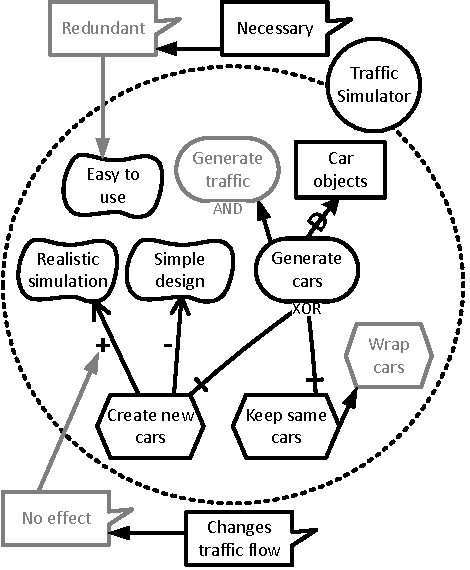
\includegraphics[width=\columnwidth]{img/Example1-new-attack.pdf}
\caption{Example RationalGRL model (extension of Fig.~\ref{fig:example-small})}
\label{fig:example-small3}
\end{figure} 

\begin{definition}[Generic Argument]
\label{def:generic-argument}
A generic argument is a tuple $ga=(id, type, name)$, where:
\begin{itemize}
\item $id\in \mathbb{N}$ is the identifier of the generic argument,
\item $type = GenArg$ states that the tuple is a generic argument,
\item $name\in Names$ is a string description of its name.
\end{itemize}
A set of generic arguments is denoted by $GA$.
\end{definition}

Thus, a generic argument is any element in the RationalGRL model that is not an intentional element or an actor. In the example, some of the generic arguments are $(13, GenArg, \text{Redundant})$ and $(14,$ $GenArg,$ Necessary$)$. Note that a constraint of a GRL model (Definition~\ref{def:grl-model}) is that GRL links should connect IEs, which means that in generic arguments cannot be connected with GRL links. 
 
We can now define \emph{arguments}. 

\begin{definition}[Argument]
\label{def:argument}
An argument $A$ is on of the following tuples:
\begin{itemize}
\item An intentional element $ie$ (Def.~\ref{def:ie}), 
\item An actor $act$ (Def.~\ref{def:actor}),
\item An Actor-IE relation $r_{ActIE}$ (Def.~\ref{def:act-ie-relation}), 
\item A link $link$ (Def.~\ref{def:link}),
\item A generic argument $ga$ (Def.~\ref{def:generic-argument}).
\end{itemize}
\end{definition}

This definition captures the specification in the RationalGRL metamodel (Figure~\ref{fig:metamodel}) in which the class \textsf{Argument} is a superclass of \textsf{GenericArgument} and \textsf{GRLModelElement}. In sum, we define an argument simply as any one of the GRL IEs or links, or a generic argument. 

Examples of arguments in Figure~\ref{fig:example-small3} are $A_5 = (5,$ $Goal,$ Generate cars$, AND)$, $A'_5 = (5, Goal,$ Generate cars$, XOR)$, $A_4 = (4, Softgoal,$ Easy to use) and $A_{13}=(13,$ $ArgElem,$ Redundant$)$. Note that the two arguments $A_5$ and $A'_5$ show an important difference between RationalGRL models and valid GRL models: While a valid GRL model disallows multiple elements with the same identifier (Definition~\ref{def:valid-grl-model}, condition 1), RationalGRL models do not enforce this restriction. This is because it is possible to create multiple arguments for the same element, where each argument contains different content for the same element. However, the set of \emph{accepted} elements in a RationalGRL should all have unique identifier (see Definition~\ref{def:valid-rationalgrl-model}).

\begin{definition}[Attack Link]
\label{def:link:attack}
Given a set of arguments $Arg$, an attack link $att=(A_i,A_j)$ means:
\begin{itemize}
\item $A_i\in Arg$ is the argument performing that attack,
\item $A_j\in Arg$ is the argument being attacked.
\end{itemize}
A set of attack links is denoted by $Att$.
\end{definition}

As an example, take the arguments $A_5$ for the goal `Generate cars' ($AND$ decomposition), $A'_5$ for the goal `Generate cars' ($XOR$ decomposition), $A_4$ for the softgoal `Easy to use' and the generic argument $A_{13}$ (`Redundant') against the softgoal (`Easy to use'). Given these arguments there are two attack links (Figure~\ref{fig:example-small3}), namely $(A'_{5},A_{5})$ and $(A_{13}, A_{4})$.

We now define a RationalGRL model.

\begin{definition}[RationalGRL Model]
\label{def:rationalgrl-model}
A \emph{RationalGRL model} $RatGRL=(Arg, Att)$ consists of a set of arguments $Args$ (Def.~\ref{def:argument}) and a set of attack links $Att$ (Def.~\ref{def:link:attack}).
\end{definition}

The definition of a RationalGRL model collects all the previously defined GRL and RationalGRL elements in a single definition. For completeness, we now provide the full specification of Figure~\ref{fig:example-small3}. Let us first enumerate all the arguments used in this example:

\begin{flalign*}
A_0 = &(0, Actor, \text{Traffic simulator})&\\
A_1 = &(1, Task, \text{Car objects}),&\\
A_2 = &(2, Softgoal, \text{Realistic simulation}),&\\
A_3 = &(3, Softgoal, \text{Simple design}),&\\
A_4 = &(4, Softgoal, \text{Easy to use}),&\\
A_5 = &(5, Goal, \text{Generate cars}, AND),&\\
A'_5 = &(5, Goal, \text{Generate cars}, XOR),&\\
A_6 = &(6, Task, \text{Create new cars}),&\\
A_7 = &(7, Task, \text{Wrap cars}),&\\
A'_7 = &(7, Task, \text{Keep same cars}),&\\
A_8 = &(8, Dep, 4, 1),&\\
A_9 = &(9, PosContr, 6, 2),&\\
A_{10} = &(10, NegContr, 6, 3),&\\
A_{11} = &(11, Decomp, 6, 5),&\\
A_{12} = &(12, Decomp, 7, 5),&\\
A_{13} = &(13, GenArg, \text{Redundant}),&\\
A_{14} = &(14, GenArg, \text{Necessary}),&\\
A_{15} = &(15, GenArg, \text{No effect}),&\\
A_{16} = &(16, GenArg, \text{Changes traffic flow}),&\\
A_{17} = &(ActIE,0,1),\ldots,A_{23}=(ActIE,0,7)&\\
\end{flalign*}
This model is then formalized as $RatGRL=(Arg, Att)$ where:
\begin{flalign*}
Arg = &\{A_0,\ldots,A_5, A'_5,A_6,A_7,A'_7\ldots,A_{23}\}\\
Att= &\{(A'_{5},A_5), (A'_{7},A_{7}), (A_{13},A_{4}), (A_{14},A_{13}),\\
     & (A_{15},A_{9}),(A_{16},A_{15})\}\\
\end{flalign*}

In Figure~\ref{fig:example-small3}, it can be read from that arguments $A_5$, $A_7$, $A_{13}$ and $A_{15}$ are currently disabled (rejected). However, we have not yet make it clear how exactly this is computed. We will do so in the following definitions.
\begin{figure}[b]
\centering
\includegraphics[]{img/Example1-new-arguments.pdf}
\caption{Example argumentation framework, subset of the RationalGRL model from Figure~\ref{fig:example-small3}.}
\label{fig:goalmodeling:arg2}
\end{figure}
In order to compute when an argument is accepted and when it is not we use argumentation semantics.  We use the standard approach by Dung~\cite{Dung1995}. 

\begin{definition}[Argumentation Framework]
\label{def:argumentation-framework}
An \emph{argumentation framework} $AF=(Arg,Att)$ consists of a set of arguments $Arg$ and a set of attack relations $Att\subseteq Arg\times Arg.$
\end{definition}

Note that the definition of a RationalGRL model (Definition~\ref{def:rationalgrl-model}) is exactly the same as the definition for an argumentation framework. This allows us to use the following definitions directly.

\begin{definition}[Attack, conflict-freeness, defense, admissibility, preferred extension] \label{def:semantics}Suppose an argumentation framework $AF=(Arg,Att)$, two sets of arguments $S\cup S'\subseteq Arg$, and some argument $A\in Arg$. We say that
\begin{itemize}
\item $S$ \emph{attacks} $A$ iff some argument in $S$ attacks $A$,
\item $S$ \emph{attacks} $S'$ iff some argument in $S$ attacks some argument in $S'$,
\item $S$ is \emph{conflict-free} iff it does not attack itself,
\item $S$ \emph{defends} $A$ iff for each $B$ such that $B$ attacks $A$, $S$ attacks $B$,
\item $S$ is \emph{admissible} iff $S$ is conflict-free and defends each argument in it.
\item $S$ is a \emph{preferred extension} iff it is a maximal (w.r.t. set inclusion) admissible set.
\end{itemize}
\end{definition}

Let us explain these definitions using the example argumentation framework in Figure~\ref{fig:goalmodeling:arg2}, which is a subset of our RationalGRL model from Figure~\ref{fig:example-small3}, containing only arguments $A_4, A_{5},A'_{5},A_{13}$, and $A_{14}$. In this example, there are five admissible sets: $\{A'_{5}\}$, $\{A_{14}\}$, $\{A'_{5},A_{14}\}$, $\{A_4, A_{14}\}$ and $\{A_4, A'_5, A_{14}\}$. In the admissible sets that contain both $A_{4}$ and $A_{14}$, we say that $A_{14}$ defends $A_4$ against its attacker $A_{13}$\footnote{In the argumentation literature, argument $A_{14}$ is often said to \emph{reinstate} argument $A_{4}$}. Sets containing both $A_{5}$ and $A'_{5}$, or both $A_{13}$ and either $A_4$ or $A_{14}$ are not conflict free. Sets containing $A_5$ are not admissible, as they do not defend $A_5$. Similarly, sets containing $A_4$ but not $A_{14}$ are not admissible as they do not defend themselves against $A_{13}$. 

The notion of admissible sets gives rise to various possible extensions of an argumentation framework; in this article, we use the preferred extension. In Figure~\ref{fig:goalmodeling:arg2}, there is one preferred extension, namely $\{A_4, A'_5, A_{14}\}$. It is possible to have multiple preferred extensions in cases where the argumentation framework contains cycles. A simple example of such an argumentation framework is shown in Figure~\ref{fig:goalmodeling:arg3}, where arguments $A_x$ and $A_y$ attack each other. There are two preferred extensions, namely $\{A_x\}$ and $\{A_y\}$. Although the algorithms in Section~\ref{sect:algorithms} do not generate mutually attacking arguments such as in Figure~\ref{fig:goalmodeling:arg3}, our formal framework does not explicitly forbid attack cycles in RationalGRL models. We discuss this in more detail in Section~\ref{sect:discussion:futurework}.

\begin{figure}[ht]
\centering
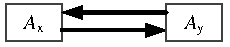
\includegraphics[]{img/example-mutual-attack.pdf}
\caption{Example of a cyclic argumentation framework.}
\label{fig:goalmodeling:arg3}
\end{figure}

The status of individual arguments can now be determined on the basis of the preferred extensions. Recall from the metamodel (Figure~\ref{fig:metamodel}) that an argument can be \emph{acceptable}, \emph{undecided} or \emph{rejected}. 

\begin{definition}[Argument Acceptability] 
\label{def:acceptability}
\begin{itemize}
\item An argument is \emph{acceptable} w.r.t. an argumentation framework $AF$ if it is in every preferred extension of $AF$. 
\item An argument is \emph{undecided} w.r.t. an argumentation framework $AF$ if it is in at least one but not all preferred extensions of $AF$. 
\item An argument is \emph{rejected} w.r.t. an argumentation framework $AF$ if it is in no preferred extension of $AF$. 
\end{itemize}
\end{definition}

Take our two simple examples. In Figure~\ref{fig:goalmodeling:arg2}, we have that arguments $A_4$, $A'_5$ and $A_{14}$ are acceptable and arguments $A_5$ and $A_{13}$ are rejected. In Figure~\ref{fig:goalmodeling:arg3}, both arguments $A_x$ and $A_y$ are undecided. Returning to our larger example from Figure~\ref{fig:example-small3}, we can see that arguments $A_5$, $A_7$, $A_{13}$ and $A_{15}$ are rejected and all the other arguments are acceptable.

Note that argument acceptability is essentially a three-valued (or binary if one does not count \emph{undecided}) concept. There are many more fine-grained ways of defining the acceptability of arguments using, for example, probabilities \cite{li2011probabilistic} or counting the number of attacks \cite{grossi2015graded}. However, the ``basic'' argumentation frameworks, and in particular the  have been shown to be close to how humans reason \cite{rahwan2010behavioral}. 

\subsection{Translating between RationalGRL and GRL}
\label{sect:formalframework:translation}

Now that we have formalized both a GRL model and a RationalGRL model, we present algorithms to translate between these two models. Both of these two translation algorithms are straightforward, which is result of the fact that the two models are formalized in a very similar way.

\paragraph{GRL to RationalGRL Translation} We start with the translation algorithm from GRL to RationalGRL, which is shown in Algorithm~\ref{alg:translation:to-rationalgrl}. The translation algorithm takes a GRL model $GR=(IE, Act, R_{ActIE}, Link)$ (Definition~\ref{def:grl-model}) as input. On line~\ref{alg:translation:to-rationalgrl:args}, it collects all the elements of the GRL model into a set $Arg$, which represents the set of arguments of the RationalGRL model. On line~\ref{alg:translation:to-rationalgrl:att}, the set of attack links is initialized with an empty set, and the new RationalGRL model $(Arg, Att)$ is returned on line~\ref{alg:translation:to-rationalgrl:return}.

\begin{algorithm}[ht]
  \caption{GRL to RationalGRL Translation}
  \label{alg:translation:to-rationalgrl}
  \begin{algorithmic}[1]
    \Procedure{$ToRationalGRL$}{$GRL$}
    \State $Arg \leftarrow IE\cup Act \cup R_{ActIE}\cup Link$\label{alg:translation:to-rationalgrl:args}
    \State $Att \leftarrow \emptyset$\label{alg:translation:to-rationalgrl:att}
    \State \Return $(Arg, Att)$\label{alg:translation:to-rationalgrl:return}
    \EndProcedure
  \end{algorithmic}
\end{algorithm}

\paragraph{RationalGRL to GRL translation} The translation from a RationalGRL model to a GRL model is given in Algorithm~\ref{alg:translation:to-grl}. First. the arguments are each put in the corresponding GRL component sets. The procedure $ComputeExtensions(Arg,Att)$ (line~\ref{alg:translation:to-grl:extension}) computes the (preferred) extensions of the RationalGRL model (Definition~\ref{def:semantics}). A GRL model is then generated from each of the preferred extensions. This is done by iterating over all arguments in the extension in line~\ref{alg:translation:to-grl:for}. The switch statement on line~\ref{alg:translation:to-grl:switch} then does a case distinction on the type of the arguments -- here, $Arg.type$ refers to the $type$ element in an argument tuple $Arg$ -- and each case ensures the argument is put in the right GRL component. Finally, the algorithm returns a GRL model on line~\ref{alg:translation:to-grl:return}. As an example, compare the RationalGRL model in Figure~\ref{fig:example-small3} to the GRL model in Figure~\ref{fig:example-small}, where the latter is a translation of the former.

\paragraph{Valid RationalGRL model} While we have defined a notion of a \emph{valid GRL model} (Definition~\ref{def:valid-grl-model}), we have not done so for a RationalGRL model yet. We define a RationalGRL model as valid if and only if the RationalGRL to GRL translation results in a valid GRL model. Thus, we do not have to reiterate all conditions on a GRL model, but use the translation algorithm.

\begin{algorithm}[b]
  \caption{RationalGRL to GRL Translation}
  \label{alg:translation:to-grl}
  \begin{algorithmic}[1]
    \Procedure{$ToGRL$}{$RatGRL$}
    \State $Ext \leftarrow ComputeExtensions(Arg,Att)$\label{alg:translation:to-grl:extension}
    \For{$E \in Ext$} 
    \State $IE\leftarrow\emptyset$, $Act\leftarrow\emptyset$, $R_{ActIE}\leftarrow\emptyset$, $Link\leftarrow \emptyset$
    \For{$A\in E$}\label{alg:translation:to-grl:for}
      \Switch{$A.type$}\label{alg:translation:to-grl:switch}
          \Case{$IETypes$}
            \State $IE\leftarrow IE\cup \{A\}$
          \EndCase
          \Case{$Actor$}
            \State $Actor\leftarrow Actor\cup \{A\}$
          \EndCase
          \Case{$ActIE$}
            \State $ActIE\leftarrow ActIE\cup \{A\}$
          \EndCase
          \Case{$LinkTypes$}
            \State $Link\leftarrow Link \cup\{A\}$
          \EndCase
      \EndSwitch
    \EndFor
    \State \Return $(IE,Act,R_{ActIE}, Link)$\label{alg:translation:to-grl:return}
    \EndFor
    \EndProcedure
  \end{algorithmic}
\end{algorithm}

\begin{definition}[Valid RationalGRL Model]
\label{def:valid-rationalgrl-model}
A RationalGRL model $RatGRL = (Arg, Att)$ (Def.~\ref{def:rationalgrl-model})
is a \emph{valid RationalGRL model} iff $ToGRL(RatGRL)$ (Algorithm~\ref{alg:translation:to-grl}) is a valid GRL model (Def.~\ref{def:valid-grl-model}).
\end{definition}


\subsection{Algorithms for argument schemes and critical questions}
\label{sect:algorithms}

We have now formalized a \emph{static} representation of the RationalGRL framework. In this section we formalize algorithms for applying argument schemes and critical questions. These algorithms are applied to RationalGRL models (Definition~\ref{def:rationalgrl-model}) and produce new arguments and attack relations. 

As discussed in Section~\ref{sect:overview}, the argument schemes and critical questions of Table~\ref{table:argument-schemes} all lead to one of three operations: \textsf{INTRO}
introduces a new RationalGRL element and \textsf{DISABLE} creates a new argument that attacks another argument. The \textsf{REPLACE} operation can be seen as a combination of \textsf{INTRO} and \textsf{DISABLE}: a new argument corresponding to a GRL element is added and this new argument attacks a previous version of the element or link. We will discuss all three operations in separate sections below.

In all of the following algorithms, we assume that:
\begin{itemize}
\item The algorithms are applied to some valid RationalGRL model $RatGRL$ (Definition~\ref{def:valid-rationalgrl-model}),
\item The procedure $mintId()$ generates a new unique id.
\end{itemize}

\subsubsection{INTRO algorithms}
\label{sect:formalframework:intro}

The following arguments schemes and critical questions of Table~\ref{table:argument-schemes} fall into this category:
\begin{itemize}
\item AS0-AS12
\item CQ5b, CQ6b, CQ6c, CQ7b, CQ9, CQ10b
\end{itemize}

These type of algorithms are short, and consist simply of adding an argument for the element that is being added. We illustrate this with a single example algorithm for AS5.

\begin{algorithm}[h]
  \caption{AS5: Goal with id $i$ decomposes into task $T$}\label{alg:add-decomp}
  \begin{algorithmic}[1]
    \Procedure{$AS_5$}{$i, T$}
    \State $task\_id\gets mintId()$\label{alg:add-decomp:task-id}
    \State $A_1\leftarrow (task\_id, Task, T)$\label{alg:add-decomp:arg1}
    \State $A_2\leftarrow (mintId(), Decomp, i, task\_id)$\label{alg:add-decomp:arg2}
    \State $Arg\gets Arg\cup \{A_1,A_2\}$\label{alg:add-decomp:add-arg}
    \EndProcedure
  \end{algorithmic}
\end{algorithm}

We have slightly reworded critical question AS5 in Algoritm~\ref{alg:add-decomp}. We assume that a goal $G$ exists already with identifier $i$, and that some new task with name $T$ is a decomposition of $G$. In the algorithm, on line~\ref{alg:add-decomp:task-id} a unique identifier is created for the task, which is created on line~\ref{alg:add-decomp:arg1}. On line~\ref{alg:add-decomp:arg2} an argument is created for the decomposition link $(mintId(), Decomp, i, task\_id)$ (Def.~\ref{def:link}, going from the existing goal with identifier $i$ to the new task with identifier $task\_id$. On line~\ref{alg:add-decomp:add-arg} the two arguments are added to the set of arguments $Arg$.

As an example, suppose we are adding the decomposition of goal ``Generate cars'', expressed as argument $A_5 = (5,$ $Goal,$ Generate cars$, AND)$, into task ``Keep same cars'', and suppose we have the following argument for the goal: . Adding the decomposition can be formalized as executing $AS_5(5, \text{Keep same cars})$, and results in two new arguments: $A_7 = (7, Task, \text{Keep same cars})$ and $A_{12} = (12, Decomp, 7, 5)$, which are both added to the set of arguments $Arg$.

The critical questions of type \emph{INTRO} are all very similar, with one exception: they require an answer. For instance, suppose CQ5b: ``Does goal $G$ decompose into other tasks?'' is answered with: ``Yes, namely into task $T$''. In this case, we simply obtain an instantiation of argument scheme AS5: ``Goal $G$ decomposes into task $T$'', which can be executed with Algorithm~\ref{alg:add-decomp}. This is the same for all the other critical questions of type \emph{INTRO}. Therefore, they are not shown here as well.

\subsubsection{DISABLE algorithms}
\label{sect:formalframework:disable}
As discussed before, algorithms of type \emph{DISABLE} consist of adding a new argument attacking an existing argument. The argument that is added is not an argument for a GRL element or link, but it is rather a generic argument (Definition~\ref{def:generic-argument}).

In the following algorithm, we assume the critical question is answered affirmatively, as indicated in the right-most column of Table~\ref{table:argument-schemes}. For instance, for critical question CQ0 ``Is the actor relevant?'', we assume it is answered with ``No''. In this case, an action is required. In contrary, if the answer to the question is ``Yes'', no action is required.

\begin{algorithm}[h]
  \caption{CQ0: Is actor with id $i$ relevant? No}\label{alg:actor-not-relevant}
  \begin{algorithmic}[1]
    \Procedure{$CQ_0$}{$i$}
    \State $A \leftarrow (mintId(),GenArg,CQ0)$\label{alg:actor-not-relevant:genarg}
    \State $Arg\leftarrow Arg \cup \{A\}$\label{alg:actor-not-relevant:genarg2}
    \For{$A_j\in \{A=(i,Actor,n)\mid A\in Arg\}$}\label{alg:actor-not-relevant:for}
      \State $Att \leftarrow Att \cup \{(A,A_j)\}$\label{alg:actor-not-relevant:att}
    \EndFor
    \EndProcedure
  \end{algorithmic}
\end{algorithm}

Algorithm~\ref{alg:actor-not-relevant} is executed when critical question CQ0 is answered with ``No''. First, on lines~\ref{alg:actor-not-relevant:genarg} and~\ref{alg:actor-not-relevant:genarg2}, an argument is created for the critical question and added to the set of arguments $Arg$. Since this argument is not an argument for a GRL element or link, it is formalized as a \emph{generic counterargument} $(mintId(), GenArg, CQ0)$ (Def.~\ref{def:generic-argument}). The for loop starting at line~\ref{alg:actor-not-relevant:for} then iterates over all arguments for actors, where $i$ is the id of the actor that is no longer relevant. The reason why there could be multiple of such actors is that the actor can be refined by an algorithm of type \emph{REPLACE}. We will explain this in more detail in the example below. Then, on line~\ref{alg:actor-not-relevant:att}, an attack link is created from the generic argument $A$ to the argument for the actor $A_j$. After executing the algorithm, all existing arguments for the actor with identifier $i$ are attacked by a newly created argument $A$.

Consider for example the RationalGRL model in Figures~\ref{fig:examples:relevant-actor}, which consists of an actor and a generic counterargument. Let us reconstruct this model using the application of argument schemes and critical questions to an initially empty RationalGRL model ($Arg=\emptyset$ and $Att=\emptyset$). The algorithm $AS_0(\text{Development team})$ is executed, which results in $A_1=\{(0,Actor,\text{Development team}\})$. After this, critical question CQ0: ``Is the actor Development team relevant?'' is answered with ``No, because the professor develops the software''. We can formalize this as executing algorithm $CQ_0(0)$ (Algorithm~\ref{alg:actor-not-relevant}), which results in adding a generic counter argument $A_2=(1, GenArg, \text{CQ0: Professor develops software})$ and an attack link $(A_2,A_1)$. The RationalGRL model now consists of two arguments, and that the preferred extension is $\{A_2\}$, which means that the resulting GRL model is empty, because generic arguments are not translated to GRL.

Algorithms for the remaining critical questions are omitted here since they are not very complex. 

\begin{figure*}[b]
\centering
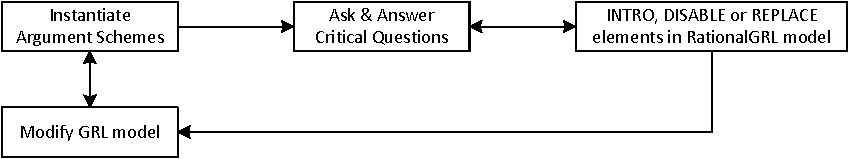
\includegraphics{img/methodology.pdf}
\caption{The RationalGRL Development Process}
\label{fig:rationalgrl-methodology}
\end{figure*}

\subsubsection{REPLACE algorithms}
\label{sect:formalframework:replace}

Recall that \emph{REPLACE} algorithms create a new argument that attacks all arguments for an existing element.

\begin{algorithm}[h]
  \caption{CQ5c: Is the decomposition type of element $ie_i$ correct? No, it should be $X$ }\label{alg:replace1}
  \begin{algorithmic}[1]
    \Procedure{$CQ_{Decomp}$}{$ie_i, X$}
    \State $A \leftarrow ie_i$\label{alg:replace1:arg}
    \State $A.decomptype\leftarrow X$\label{alg:replace1:decompchange}
    \State $IEArgs\leftarrow IE_i\subseteq  Arg$\label{alg:replace1:ieargs}
    \For{$\{(A_i,A_j)\in Att\mid A_j\in IEArgs\}$}\label{alg:replace1:for1}
      \State $Att\leftarrow (A_i,A)$
    \EndFor
    \For{$\{(A_i,A_j)\in Att\mid A_i\in IEArgs\}$}\label{alg:replace1:for2}
      \State $Att\leftarrow (A,A_j)$
    \For{$A_i\in IEArgs$}\label{alg:replace1:for3}
      \State $Att \leftarrow Att \cup \{(A,A_i)\}$\label{alg:replace1:att}
    \EndFor
    \EndFor
    \State $Arg\leftarrow Arg \cup \{A\}$\label{alg:replace1:addarg}
    \EndProcedure
  \end{algorithmic}
\end{algorithm}

While the original critical question CQ5c is specific to the decomposition between a goal and a task, Algorithm~\ref{alg:replace1} is more generally applicable to the decomposition type of any IE, since all IEs have a decomposition type (Definition~\ref{def:ie}). 

Let us go through this algorithm step by step. On line~\ref{alg:replace1:arg}, a new argument $A$ is created which is identical to original IE. On line~\ref{alg:replace1:decompchange} the decomposition type of the argument is changed to $X$ -- here, $Arg.decomptype$ refers to the $decomptype$ element in an argument tuple $Arg$. On line~\ref{alg:replace1:ieargs}, the set $IEArgs$ is assigned with all existing arguments for the input IE -- here $IE_i$ is the set of all IEs with id $i$. The first two for loops on respectively lines~\ref{alg:replace1:for1} and~\ref{alg:replace1:for2} ensure that all attack links that existing from and to the previous versions of the IE are also carried over to the new argument $A$. Then, in the third for loop on line~\ref{alg:replace1:for3}, we add attack links from the argument that has just been created to all existing arguments for the IE. This ensures that all previous version of the IE are not part of the preferred extension, and as a result do not show up in the resulting GRL model. Finally, one line~\ref{alg:replace1:addarg}, the new argument is added to the set of arguments.

As an example, take Figure~\ref{fig:example_AS}. The initial RationalGRL model (before applying CQ10b), can be formalized as follows: $RatGRL=(Arg,Att)$, with $Arg=\{A_1,A_2,A_3,A_4,A_5\}$ and $Att=\emptyset$, where:
\begin{itemize}
\item $A_1=(0,Goal,\text{Simulate traffic},AND)$
\item $A_2=(1,Task,\text{Dynamic simulation},AND)$
\item $A_3=(2,Task,\text{Static simulation},AND)$
\item $A_4=(3,Decomp,1,0)$
\item $A_5=(4,Decomp,2,0)$
\end{itemize}

Suppose algorithm $CQ_{Decomp}(0, XOR)$ is executed for this RationalGRL model. On lines~\ref{alg:replace1:arg} and \ref{alg:replace1:decompchange} a new argument $A_6=(0,Goal,\text{Simulate traffic},OR)$ is created. On line~\ref{alg:replace1:ieargs}, $IEArgs$ contains all arguments for element 0, which is $\{A_1\}$ (note this does not yet include argument $A_6$, since it is not yet added to the RationalGRL model). The first two for loops on lines~\ref{alg:replace1:for1} and~\ref{alg:replace1:for2} do not do anything in the case of our example, since $A_1$ is itself not attack or does not attack any other argument. The for loop on line~\ref{alg:replace1:for3} ensures all previous versions of the element with id 0 are now attacked, which means in our case the $(A_6,A_1)$ is added to $Att$. Finally, on line~\ref{alg:replace1:addarg} the new argument $A_6$ is added to $Arg$.

The other \emph{REPLACE} algorithms are similar to Algorithm~\ref{alg:replace1}, which can be used directly for CQ10c. For CQ12 we should make a small modification: instead of replacing the decomposition type of the IE, we replace its name. Since this is a very minor modification we don't show it here.
\section{The RationalGRL Tool}
\label{sect:tool}

An important requirement of our framework is that it has tool support. This is for various reasons: i) although there are various approaches attempting to combine goal modeling with argumentation, there does not yet exist any tool support (see Section~\ref{sect:discussion}), ii) it allows us to do user tests in future research, exploring the difference between GRL and RationalGRL, iii) tool support is an excellent verification to ensure our formal framework and algorithms actually work, iv) having a light-weight web-based version of GRL is useful for the community in general.

GRL has a well-documented and well-maintained tool called jUCMNav~\cite{jUCMNav}. This tool is an extension to Eclipse. Although it is a rich tool with many features, it is implemented as an Eclipse plugin. We have experienced on various occasions that setting this up properly can take up a significant time of experiments, leaving less time for actual modeling.

In this section we present our web-based prototype of RationalGRL. It can be accessed from:
\begin{quote}
\url{http://www.rationalgrl.com}
\end{quote}

The tool is written in Javascript, and runs on all modern browsers. The tool is open-source, and the source can be accessed from:
\begin{quote}
\url{http://www.github.com/marcvanzee/RationalGRL}
\end{quote}

In this section we briefly highlight some features of the language, and we explain some of its current limitations.

\todo{all}{marc}{Explain figures in Appendix~\ref{sect:tool-screenshots}}
\section{RationalGRL user evaluation}
\label{sect:validation}

In addition to the empirical case study (Section~\ref{sect:gmas}), which forms the basis of the RationalGRL framework, we also performed a user evaluation with 16 users. The objective of this evaluation was to determine whether the users found the additions of RationalGRL (arguments, argumentation semantics, critical questions) useful compared to standard GRL, and whether they found it easier to keep track of and express opinions and beliefs using RationalGRL compared to standard GRL. Regarding the comparison of RationalGRL to GRL, the following two broad hypotheses follow from our main points in this paper:

\begin{itemize}
\item[H1] The additions of RationalGRL -- arguments, critical questions and determination of the status of arguments -- are a useful addition to standard goal modelling in GRL.
\item[H2] The additions of RationalGRL make it easier to express, determine the effect of and communicate to other stakeholders one's opinions and beliefs about a goal model.
\end{itemize}

In addition, we wanted to know whether the RationalGRL tool was difficult or easy to use. Note that we did not aim to conduct a usability study for the RationalGRL tool. Rather, we were interested to know if the tool was clearly very easy or difficult to use, as this could influence the participants ideas about the RationalGRL framework and language -- a very nice and easy to use tool tends to make people more positive twoards a particular modelling language, whereas irritations about a bad or buggy tool will lead to a more negative disposition. This leads to the following general hypothesis:

\begin{itemize}
\item[H3] The usability of the RationalGRL tool is neither (very) easy or (very) difficult. 
\end{itemize}

In the rest of this section, we will describe our experiment in more detail and further specify these hypotheses.

\subsection{Experiment design}

The idea was to have our participants perform a small modelling task, and then ask them what they thought of RationalGRL and the tool. Thus, our experiment consisted of three parts:

\begin{enumerate}
\item Explanation: We explain to the participants the basics of the RationalGRL development process and the RationalGRL tool.
\item Modeling: We ask the participants to model a summarized discussion in the RationalGRL tool.
\item Survey: We present the participants with a survey containing questions about the comparison between RationalGRL and GRL, and questions about the usability of the RationalGRL tool.
\end{enumerate}

The instructions for these three parts are contained in a single document that we sent out to the participants.\footnote{See \url{www.rationalgrl.com}, page ``Empirical Study''} The explanation (part 1) starts with a general explanation of GRL and standard goal modelling similar to the explanation provided in section \ref{{sect:background:grl}, then briefly discusses the additions of RationalGRL (argument, attack, critical questions) and finally the tool is briefly described (similar to Section \ref{sect:tool}). 

For part 2, we provided a small part of a transcript and some context information (see Appendix~\ref{sect:survey}) and asked the participants to model this in the tool and take a screenshot of their final model. The idea is that the participants are ``present'' at a discussion about the early-stage requirements and are asked to model the goal model corresponding to these requirements. 

For part 3, we provided the participants with a survey\footnote{https://goo.gl/forms/fDSMUnAV20wy7kbY2} . The survey starts with general questions about the participant (experience etc.). It then asks the following questions about the RationalGRL tool, asking the participants to rate various aspects of the tool on a Likert scale of 1 (very difficult) to 5 (very easy):
\begin{itemize}
\item[Q1] Was it easy or difficult to get started with the RationalGRL tool?
\item[Q2] Was the details pane (containing details of an element, critical questions, etc) easy or difficult to use?
\item[Q3] Was it easy or difficult to understand the way in which the status of arguments and other elements is determined?
\item[Q4] Did you find it easy or difficult to model the example discussion using RationalGRL?
\end{itemize}
We also ask open questions about the strengths and weaknesses of the tool, possible improvements and whether the participant thinks the tool could in the future be used in practice.

The second part of the survey concerns the comparison between GRL and RationalGRL and starts with Figure~\ref{fig:example-small}, which models the discussion for part 2 (Appendix~\ref{sect:survey}) in standard GRL, so that the participants can compare their own RationalGRL models and experiences with the standard GRL model. The following questions ask the participants to rate RationalGRL on a Likert scale from 1 (very useless) to 5 (very useful):
\begin{itemize}
\item[Q5] Do you think the arguments and counterarguments of RationalGRL are a useful extension to standard goal modeling?
\item[Q6] Do you think the critical questions and answers in the details pane are a useful extension to standard goal modeling?
\item[Q7] Do you think the automatic determination of the status of arguments and elements is a useful extension to standard goal modeling?
\end{itemize}
The following questions ask the participants to rate RationalGRL vs. standard goal modelling on a Likert scale from 1 (much more difficult) to 5 (much easier):
\item[Q8] Do you think using RationalGRL instead of a standard goal modeling language makes it easier or more difficult to for someone to express beliefs and opinions in a goal model?
\item[Q9] Do you think using RationalGRL instead of a standard goal modeling language makes it easier or more difficult to for someone to determine the effect of beliefs and opinions on the resulting goal model?
\item [Q10] Do you think using RationalGRL instead of a standard goal modeling language makes it easier or more difficult to for someone who is not the original author to understand the goal model? 
\end{itemize}
We conclude with two open questions regarding the strengths and weaknesses of RationalGRL compared to GRL.

\paragraph{Participants}
We asked 16 participants in our network to participate in our experiment. Most of the participants were therefore either employed at the first author's company or staff and (ex-)students from the second author's university. Hence, two thirds of the participants had either a PhD or Master degree, 20\% a Bachelor degree, and one respondent responded with ``Other''. All but one participant had a year or more experience with software development. The average experience was 6.2 years (standard deviation 6.7), with 10 participants having less than 5 years of experience and 6 participants having 8 or more years of experience, with one participant having 25 years of experience. The participants also judged themselves to be quite competent in  early-phase requirements engineering: on average they gave themselves a rating of 3.2 out of 5 (standard deviation 1.3) with half of the participants claiming they were at least ``competent'' (rating 4) or ``very competent'' (rating 5). However, experience with goal modeling languages was markedly less: the average rating was 1.9 (standard deviation 1.3), with 9 participants claiming never to have used a goal modeling language (rating 1), and only two participants displaying regular use (monthly, rating 4, or weekly, rating 5). The participants that had experience with goal modelling languages had mostly used i* (5 users), with 2 users being familiar with GRL and 2 users having used another goal modelling language.

\subsection{Results}

In task 2, users clearly made use of the extra features offered by the RationalGRL tool: they used the details pane more often than not (rating 3.2 out of 5) and on average produced 3 arguments from the short transcript. Some of the examples of RationalGRL models the users created can be found in Appendix~\ref{sect:survey-screenshots}.

\begin{table*}[t]
\centering
\begin{tabularx}{0.95\textwidth}{l|l|l|l|l|l|l|l}
& very useless & useless & neither useful nor useless & useful & very useful & avg. score (1-5) & std. dev.\\
\hline
Q5 & 0 (0\%) & 0 (0.0\%) & 3 (21.4\%) & 8 (57.1\% & 3 (21.4\%) & 4.0 & 0.68\\
Q6 & 0 (0.0\%) & 3 (21.4\%) & 3 (21.4\%) & 6 (42.9\%) & 2 (14.3\%) & 3.5 & 1.0\\
Q7 & 0 (0\%) & 0 (0\%) & 2 (14.3\%) & 7 (50.0\%) & 5 (35.7\%) & 4.2 & 0.7
\end{tabularx}
\caption{Participant ratings of the usefulness of the additions of RationalGRL}
\label{table:survey:table2}
\end{table*}

\begin{table*}[t]
\centering
\begin{tabularx}{0.95\textwidth}{l|l|l|l|l|l|l|l}
& much more difficult & more difficult & neither more difficult nor easier & easier & much easier & avg. score (1-5) & std. dev.\\
\hline
Q8 & 0 (0\%) & 0 (0.0\%) & 3 (21.4\%) & 8 (57.1\% & 3 (21.4\%) & 4.0 & 0.68\\
Q9 & 0 (0.0\%) & 3 (21.4\%) & 3 (21.4\%) & 6 (42.9\%) & 2 (14.3\%) & 3.5 & 1.0\\
Q10 & 0 (0\%) & 0 (0\%) & 2 (14.3\%) & 7 (50.0\%) & 5 (35.7\%) & 4.2 & 0.7
\end{tabularx}
\caption{Participant ratings of whether the additions of RationalGRL make reasoning about a goal model easier}
\label{table:survey:table2}
\end{table*}

\begin{table*}[t]
\centering
\begin{tabularx}{0.95\textwidth}{l|l|l|l|l|l|l|l}
& very difficult & difficult & neither difficult nor easy & easy & very easy & avg. score (1-5) & std. dev.\\
\hline
Q1 & 2 (12.5\%) & 1 (6.3\%) & 6 (37.5\%) & 6 (37.5\% & 1 (6.3\%) & 3.2 & 1.1\\
Q2 & 2 (12.5\%) & 2 (12.5\%) & 4 (25\%) & 8 (50\%) & 0 (0\%) & 3.1 & 1.1\\
Q3 & 0 (0\%) & 3 (20\%) & 4 (26.7\%) & 5 (33.3\%) & 3 (20\%) & 3.3 & 1.4\\
Q4 & 2 (12.5\%) & 5 (31.3\%) & 6 (37.5\%) & 3 (18.8\%) & 0 (0\%) & 2.6 & 1.0
\end{tabularx}
\caption{User scores for the usability of the RationalGRL tool}
\label{table:survey:table1}
\end{table*}

Table~\ref{table:survey:table1} shows the respondents' answers, the average score, and the standard deviation for each answer. On average, the respondent found the tool relatively easy to use, but there were also a number of users that had some trouble getting started (in 3 out of the 4 questions, 12.\%5 rated ``very difficult''). We think this is not unexpected, as the cognitive burden for our framework is higher than for other goal modeling languages such as GRL and i*, simply because there are more elements in the language. Still, the majority of the users did not found the tool difficult to use.

We also asked the users three open questions related to usability. When asked about the strengths and weaknesses of RationalGRL, users where generally positive about RationalGRL's clear UI and the fact that arguments can be combined with goal models. For instance, one user stated that RationalGRL successfully ``tries to capture the rationale behind the modeling process' and ``has a simple way to compute the status of the arguments''. On the other hand, some of the users found it challenging to decide when to use arguments, and to determine when an arguments attacks another argument. For instance, a user mentioned ``it wasn't very easy because I didn't always know how to attack the elements'', and ``I don't think its necessary to include all the arguments because some of them are a bit trivial''. Other users were worried about the cognitive overload of the tool. One user mentioned ``I still believe in the value of arguments, but there should be less confusing ways to capture them''. 

When asked about improvements in the RationalGRL tool, the users mentioned additional UI functionalities such as the possibility to save models, having an ``undo'' function, and flipping the arrow after adding them. Users also suggested various language-related improvements. Some users mentioned they missed the possibility to attack links, while others mentioned that not all GRL elements are supported (for instance, it is currently not possible to add actors).

When asked whether the users believe a more mature version of RationalGRL can be used to capture early-phase requirements in an actual software development project, most users responded positively. This was somewhat surprising, since our tool is still an early prototype. Users' responses include ``Yes, having the possibility to add arguments seems quite useful'', ``I think it can, but maybe try to find a way to combine it with more regular/mainstream requirements gathering such as user stories and customer journeys'', ``yes, because it creates a clear scope for the project, what the goals are'', and ``Generally I think its useful to explicitly document arguments of a discussion''. The concern that the modeling process may involve too much cognitive overhead was mentioned again though: ``I think the overhead of inputting a (detailed) discussion in a structured manner into any system makes adoption difficult'', and ``the manual input is too complex and takes too much time. An automated process of parsing the conversation log would be much more helpful''. 

Table~\ref{table:survey:table2} shows the respondents' answers, the average score, and the standard deviation for each answer. On average, the users were positive about the usefulness of the RationalGRL extension. The rating for the usefulness of determining the status of arguments was particularly positive (rating 4.2 out of 5), which provides some indication to the fact that using argumentation semantics to be able to determine precisely which elements of a goal model are accepted could be useful in practice.

We concluded with two open questions about the comparison between RationalGRL and other goal modeling languages. When asked about the advantages of RationalGRL over standard goal modeling languages, many users agreed that making arguments explicit may force end users to have a more structured discussion: ``	Clear communication about argumentation and forcing people to think in those clear terms.'', ``...you can add arguments and that you can answer questions that help you to develop arguments'', ``It's useful that discussion and explanation are close to the diagrams'', ``a way to see how decisions are being shaped.''. When asked about the weaknesses, users mentioned the complexity as the most important weakness: ``The apparent increase in complexity might lead to negative perceptions'', ``adding yet another layer of complexity scares me''. One user mentioned that this may be a problem with goal modeling in general: ``Goal models are already complex (...) I have worked for years on the effect of context on goal models, and my conclusion is that this was very interesting academic work but with close-to-zero practical implications, unfortunately.''.

\subsection{Analysis and discussion}
In order to test our main hypotheses H1, H2 and H3, we have to formulate null hypotheses and alternative hypotheses that can be tested. For H1 and H2, we hypothesize that the participants will, on average, rate the additions of RationalGRL as useful (rating 4) or very useful (rating 5) for Q5, Q6 and Q7, and as making it easier (rating 4) or significantly easier (rating 5) for questions Q8, Q9 and Q10. In other words, we say that our null hypothesis and alternative hypothesis for H1 and H2 are as follows:
\begin{itemize}
[] H1$_{0}$ and H2$_{0}$: average rating for questions Q5-Q10 is 3 or lower.
[] H1$_{a}$ and H1$_{a}$: average rating for questions Q5-Q10 is higher than 3.
\end{itemize}

For hypothesis H3, we do not claim that the usability of the tool is especially easy or difficult: we expect the average rating for questions Q1-Q4 to not be significantly higher or lower than 3 (neither easy or difficult). Thus, our null hypothesis and alternative hypothesis for H3 are as follows:  
\begin{itemize}
[] H3$_{0}$: average rating for questions Q1-Q4 is 3.
[] H3$_{a}$: average rating for questions Q1-Q4 is not 3.
\end{itemize}

Below, we will discuss each of the hypotheses in turn.

\paragraph{Hypothesis H1}
The first analysis concerns hypothesis H1, whether the additions of RationalGRL -- arguments, critical questions and determination of the status of arguments -- are a useful addition to standard goal modelling in GRL. Our hypothesis was that on average the participants would rate the additions as either useful (rating 4) or very useful (rating 5) in question Q4, Q5 and Q6. For each separate question Q4, Q5, Q6, we can thus formulate the following null hypothesis H1$_{0}$ and alternative hypothesis H1$_{a}$.  

\paragraph{Hypothesis H2}

\paragraph{Hypothesis H3}




\subsection{Analysis}\label{sec:eval-an}
Although our empirical evaluation is relatively small-scale, and we cannot draw hard conclusions from it, we do believe that we can extract some interesting observations. We list the three most important ones:
\begin{enumerate}
\item \emph{High cognitive overhead.} A concern that was raised often in our empirical evaluation is that, in its current form, RationalGRL has a relatively high cognitive overhead. Goal modeling is by itself already a cognitively high-effort activity, and the fact that we add more elements to the language does not improve this. This may mean that in future work we should focus more on the RationalGRL development process\footnote{Note that in order to keep the study simple for the users, we did not explicitly ask the respondents to follow the development process from Section~\ref{sect:methodology}}. Users like to be guided during modeling phase, and making arguments explicit in the modeling process was indicated as useful, but argumentation should be integrated into the \emph{process} of goal modeling more than in the goal models themselves. Critical questions seem to be a natural fit for this, as they play a key role in the RationalGRL development process, but in its current form they are only mentioned in the details pane of the tool.
\item \emph{Useful argumentation semantics.} Participants were enthusiastic about adding arguments to a goal modeling language with a clear formal underpinning, and they believed the argumentation semantics we use in the tool is very intuitive. This is a positive signal for our formal approach.
\item \emph{Lightweight tool.} Respondents were positive about the fact that it was very easy to get started with the tool. Thus, it seems that having a simple web-interface for goal modeling languages is something that could be done more in the future. Most comments on the tool were the type of comments that are expected from a prototype implementation.
\end{enumerate}
\section{Discussion}
\label{sect:discussion}

\subsection{Related Work}
\label{sect:discussions:relatedwork}

\paragraph{Design Rationale} Argumentation in software design has been the subject of the research on so-called \emph{design rationale} (DR), an explicit documentation of the reasons behind decisions made when designing a system or software architecture. Starting already in the 90's with influential issue-driven design methods such as gIBIS and QOC~\cite{shum2006hypermedia},  
DR looks at issues, options and arguments for and against these options in the design of, for example, a software system. Similar to the literature on goal modeling, much of the traditional DR literature provides modeling languages and diagramming tool support for building design rationales. It is in this diagramming functionality that the link with argument diagrams from philosophy, law and AI~\cite{reed2004araucaria,gordon2007visualizing} has been made, where argument diagrams represent reasoning from premises to conclusions. One of the problems of such methods and tools is the cognitive overload that results from having to learn and use such tools at the same time as having to discuss and think about complex software designs [5]. Furthermore, not much of the research on design reasoning has empirically investigated which techniques and how much information designers use in design reasoning, which information is missing, and how the use of design reasoning techniques affects design discussions and eventually the quality of design discourse. More recent research on DR therefore moves away from the idea that all decision have to be explicitly diagrammed and focuses more on empirically investigating how critical reflection can help when designing \cite{razavian2016two,TangEtal2018}, or which parts of the design process are best explicitly documented \cite{falessi2013value}. 

Software design and requirements engineering are very closely related \cite{nuseibeh2001weaving} and hence the insights from the DR literature are directly applicable to RE. The RationalGRL framework essentially incorporates the core ideas from DR into goal-oriented requirements engineering by explicitly including arguments for and against the various options into the goal model. In this respect, we may seem to go against the trend in DR research to focus less on diagramming and more on guidelines for design processes. There are two reasons for this. First, as opposed to DR diagramming, goal modeling is still very much an active area of research \cite{GonccalvesEtal2018} with clear practical applications \cite{NeaceEtal2018}. Second, we note that RationalGRL also includes a development process and critical questions that encourage reflection when thinking about the possible goals and functionality of a system, which connects with the more research ideas on DR \cite{razavian2016two,TangEtal2018}. 

\paragraph{Requirements Engineering} 
There are numerous examples in the RE literature that make mention of arguments, questions or conflicts in some way. Already in 1997, Smith~\cite{Smith:1997:CRF:2737426.2737493} proposed a framework to develop arguments, which relates a model of a proposed software system to a model of its environment, and shows that these together achieve properties described by a model of requirements. In a similar vein, Lockerbie \emph{et al.}~\cite{lockerbie2012exploring} describe procedures that analysts follow to use satisfaction arguments in combination with $i*$. Also, Horkoff and Yu~\cite{horkoff2016interactive} introduce analysis procedures for the $i*$ goal-oriented framework, allowing users to ask questions such as ``what if?'', or ``are certain goals achievable? how? or why not?''. Finally, Hassin and Amyot~\cite{hassine2016questionnaire} analyze the correctness of GRL models by performing statistical analysis on generated questionnaires, which allows for early detection of potential conflicts between stakeholders of the system. The mentioned work, however, does not consider arguments the way RationalGRL does, that is, as explicit opinions of stakeholders. 

A number of approaches in the field of requirements engineering explicitly take into account arguments. One early example comes from Haley \emph{et al.}~\cite{haley2008security}, who use formal logical arguments to show that the system behavior satisfies certain security requirements, and more informal arguments to capture and validate the assumptions underlying the system behavior. This system behavior is defined by the tasks it executes and thus arguments are given for and against system tasks, similar to the way beliefs and counterarguments can be provided for tasks in RationalGRL. What Haley \emph{et al.} leave implicit in their argumentation are the goals of the stakeholders on which the system tasks depend -- they include the goals in their framework and mention that there will often be conflicting goals between stakeholders, but they do not explicitly model them. Furthermore, the argumentative part of their framework does not include formal semantics for resolving conflict between arguments or determining the acceptability of arguments. Yu \emph{et al.}~\cite{yu2015automated} further extend the framework by Haley \emph{et al.}, including algorithms for Dung-style argumentation semantics \cite{Dung1995} and a database of specific ways in which to attack (or mitigate) risks. This extension can be likened to a set of critical questions for risks and security requirements (cf. Yu \emph{et al.}~\cite{yu2015automated} Section 3.1).

Another recent example of the use of arguments in goal-oriented requirements engineering is the work by Murukannaiah \emph{et al.}~\cite{murukannaiah2015}, who propose Arg-ACH, where the beliefs underlying conflicting goals can be made explicit using argumentation. Murukannaiah \emph{et al.} start with the basic technique of Analysis of Competing Hypotheses (ACH), where for conflicting goals, the beliefs that are consistent and inconsistent with these goals are included in a matrix and counted. They then extend this technique into Arg-ACH: instead of just indicating whether a belief is consistent or inconsistent with a goal, each belief becomes an argument for or against the goal, which is then diagrammed using the Carneades tool \cite{gordon2007visualizing}. Belief scores are assigned to arguments, which can be aggregated to provide one's belief in a goal. The arguments for and against goals can be based on argument schemes, and critical questions can be used to find new arguments for or against the goals or the existing arguments. One example provided in the paper is the argument scheme from expert opinion, which allows one to draw conclusions based on expert statements and subsequently question, for example, the objectivity and veracity of the expert using critical questions. Murukannaiah \emph{et al.} conducted an experiment in which they had two groups, one with ACH and one with Arg-ACH, perform an analysis of several conflicting goals regarding security at transport hubs. They found that, while the group that used Arg-ACH took longer, they also covered more possibilities in their belief search and the conclusions were more consistent among the group. 

One other example of argumentation in RE concerns the use of argumentation in requirements elicitation. Ionita \emph{et al.}~\cite{ionita2014argumentation} propose a simple argumentation dialogue game in which risk assessors try to attack each other's arguments for certain risks attached to a system design. Dung's semantics \cite{Dung1995} are then used to determine the risks that are still valid, and those that have been successfully rejected. Elrakaiby \emph{et al.}~\cite{ElrakaibyFSGN17} use argumentation to explain ambiguity. They define when a statement by a client who is being interviewed about the requirements of a system presents an inconsistency or an insufficiency. An inconsistency can be either with the client's previous statements or with the requirement engineer's beliefs. An insufficiency occurs when an analyst needs more information from the client to accept a client's statement.

It is clear from this literature that arguments play a core role in RE. Murukannaiah \emph{et al.}~\cite{murukannaiah2015} show that critical reflection using argument schemes and critical questions -- in the same way that RationalGRL proposes -- improves the quality of the reasoning in the RE process. Elrakaiby \emph{et al.}~\cite{ElrakaibyFSGN17} provide a case study similar to our research, identifying, many counterarguments specifically with respect to realisability, relevance and clarity (cf. CQ2a, CQ3, CQ11 and CQ12 in Table~\ref{table:argument-schemes}). Similar to RationalGRL, the use of Dung-style argumentation semantics to compute the acceptable claims in RE is also advocated by the literature \cite{yu2015automated,ionita2014argumentation,ElrakaibyFSGN17}. 

The current work on RationalGRL puts the insights from the above-mentioned literature in a broader framework. For example, there is a specific focus on security requirements \cite{haley2008security,yu2015automated,ionita2014argumentation} or the reasoning is about single goals or tasks instead of about the wider context as represented in a goal model \cite{haley2008security,yu2015automated,murukannaiah2015,ElrakaibyFSGN17}. RationalGRL provides a generic and extensible framework for arguing about goals and tasks in RE. At the moment, there is only a ``generic argument'' in addition to arguments about goals and tasks. However, new argument schemes and critical questions about, for example, security risks or expert opinions, can be easily added: the metamodel (Figure~\ref{fig:metamodel}) accommodates this and the formal specification in Section~\ref{sect:formalframework} is set up in such a way that extending the definition of argument and adding new algorithms for specific critical questions is easy. 

\paragraph{Goal Modeling} Argumentation has already been included implicitly in existing goal modeling languages. At its core, goal modeling is a process of argumentation: high-level goals are reasons for lower-level goals, tasks and resources. Hence, refinement and decomposition techniques used in requirements engineering \cite{van2001goal} can be seen as explicit argumentation steps in the goal modeling process. Take, for example, CQ2 of PRAS (Section~\ref{sect:background:pras}), which asks whether there are alternative ways of realizing the same goal. Providing an alternative subgoal or task in a goal model is then an explicit argumentative move in the discussion. In this sense, a goal model provides a justification for itself. This idea is also prevalent in our RationalGRL framework: many arguments are in fact GRL elements, and many critical questions can be answered by introducing new GRL elements. However, as was already argued in Section~\ref{sect:introduction} (and also by \cite{Jureta:RE2008}), argumentation produces different, richer and complementary information to the goal model. The goal model is the product of a process of argumentation, and does not include, for example, goals and tasks that were at some point considered but discarded. Furthermore, for goal models, it is only possible to determine the satisfiability of goals given the possible tasks and resources; what cannot be determined is the acceptability of goals, that is, whether they are \emph{acceptable} (cf. Definition 14 given potentially contradictory opinions of stakeholders).  

More explicit rationales for goal models are included in the original GRL specification \cite{Amyot:2010:EGM:1841349.1841356} in the form of \emph{belief} elements, which can be attached to other intentional elements (goals, tasks) using the different links (positive contribution, negative contribution) of GRL. The content of a belief is a textual description, which can explain, for instance, the rationale for including a goal in a model. In this regard, they seem like arguments or reasons for the different elements in a goal model. However, in the literature the precise usage and semantics of belief elements in GRL remain unclear: according to the metamodel \cite{Amyot:2010:EGM:1841349.1841356} they can be connected to other intentional elements (including beliefs) through any type of link, but in the jUCMNav tool there is a separate \emph{belief link} for connecting beliefs to goals and tasks only, and the beliefs are not used in any of the algorithms to compute the satisfiability of goals and tasks. We are also not aware of many examples of the usage of belief elements in the literature. Thus, what it seems like is that GRL belief elements can be understood as metadata that can be attached to an element.  

Ambiguities notwithstanding, there are further advantages of using RationalGRL over GRL with belief elements. For example, in none of the GRL specifications, is it possible to attach beliefs to links between other elements thus it is not possible, for example, to provide a rationale for why some tasks positively contributes to a goal. Furthermore, the RationalGRL arguments follow clear schemes with associated critical questions explicitly tailored towards reasoning about goals and actions or tasks, while beliefs in GRL offer no further guidance as to what kinds of rationales can be given for elements in a goal model. Furthermore, beliefs in GRL seem not to influence the goal model in any way. Arguments in RationalGRL, in contrast, play an important role in forming the resulting goal model: if an element is defeated by an argument, it is not part of the resulting goal model.

\paragraph{Goal Modeling and Argumentation}

There are several contributions to the literature that explicitly relate argumentation-based techniques with goal modeling. The first line of work is by Bagheri and Ensan \cite{bagheri2011consolidating} and Mirbel and Villata \cite{MirbelVillata12} use abstract argumentation frameworks (see Definition~\ref{def:argumentation-framework}) to capture individual goals and the relations between them as modeled in a goal model, so that consistent (i.e., acceptable) subsets of goals can be computed using the relevant argumentation semantics \cite{Dung1995}. For example, if in the goal model there is a conflict between goals $G_1$ and $G_2$, there is an attack between the arguments representing these goals and hence $G_1$ and $G_2$ cannot be in the same extension. Or if there is a dependency link between $G_1$ and $G_2$, then $G_1$ should be in every extension $G_2$ is in and vice versa. AND- and OR-decomposition are also modeled as such, that is, if $G_3$ AND-decomposes into $G_1$ and $G_2$ then $G_1$ and $G_2$ should be in every extension $G_3$ is in, and if $G_3$ OR-decomposes into $G_1$ and $G_2$ then either $G_1$ or $G_2$ should be in every extension $G_3$ is in. 

Modeling goal models as argumentation frameworks allows one to compute the consistent sets of goals and tasks given a goal model. In RationalGRL, we have opted not to provide such an argumentation-theoretic semantics to goal models. The reason for this is that GRL already has quite fine-grained satisfiability semantics \cite{Amyot:2010:EGM:1841349.1841356}, which take into account conflicts, decompositions and dependencies. RationalGRL focuses on what is not captured in the work discussed above \cite{bagheri2011consolidating,MirbelVillata12}, namely the arguments and beliefs underlying a goal model, and the way these arguments and beliefs interact with the elements of the goal model. If desired, however, it would be easy to provide Dung semantics similar to \cite{bagheri2011consolidating,MirbelVillata12} for goal models, as the elements of a goal model are already arguments in RationalGRL (Figure~\ref{fig:metamodel}). 

The contribution most closely related to ours is the work by Jureta \emph{et al.}~\cite{Jureta:RE2008}. Jureta \emph{et al.} propose ``Goal Argumentation Method (GAM)'' to guide argumentation and justification of modeling choices during the construction of goal models. GAM is a high-level decision process, in which alternative solutions for an RE problem are evaluated and compared using argumentation. Jureta \emph{et al.} use a well-known fictitious example of an argumentative discussion regarding a meeting scheduler, in which a goal model is being built by the stakeholders proposing tasks, goals, and alternative solutions for goals. They include clarification as an important step in their GAM process, and discuss various types of clarity problems (vagueness, ambiguity, overgenerality, synonymy) and basic techniques for dealing with them (e.g. thesaurus checks, labeling vague expressions). 

The GAM process is essentially a generic, high-level process for problem solving, not specifically tailored towards goal modeling. In this sense, the RationalGRL Development Process in Figure~\ref{fig:rationalgrl-methodology} can be seen as a more specific version of GAM explicitly meant for goal modeling. The argument schemes and critical questions in RationalGRL provide clearer handles for goal modeling (cf. requirement 4 of our framework, Section~\ref{sect:introduction}). Furthermore, the RationalGRL framework adds full tool support for the goal modeling and reasoning process, which GAM lacks. GAM does contain more specific ways of dealing with different types of clarity problems; in RationalGRL clarification is captured as a single critical question (CQ12, Table~\ref{table:argument-schemes}). However, as argued above further critical questions can easily be added to RationalGRL if needed.

Jureta \emph{et al.}'s framework also includes an argumentation part, where reasons (justifications) for conclusions are given as formal structured arguments\footnote{Informally, a structured argument is similar to the PRAS argument in Section~\ref{sect:background:pras}, i.e., $a, b \xrightarrow{therefore} c$.}. Arguments and alternatives are then captured as structured arguments or argument diagrams with reasons for or against goals and tasks. Given these arguments the set of undefeated (i.e., acceptable) propositions can be computed to determine which alternative solution to a problem is acceptable. Thus, the arguments and beliefs underlying a goal model and possible alternative modelings are captured as formal arguments. Furthermore, a mapping from goal models to argument diagrams is given, so that it is possible to start arguing about an already existing goal model.

RationalGRL allows for two-way translation between arguments about goals and standard goal models (cf. Section~\ref{sect:formalframework:translation}). In contrast, Jureta \emph{et al.} only provide a mapping from goal models to structured arguments, and the step from structured arguments or argument diagrams to goal models is never formally defined. In previous work on the RationalGRL framework~\cite{vanzee-etal:renext2015,vanZee-etal:er2016}, we extended Jureta \emph{et al.}'s work and translated argument diagrams to GRL models (an automatic translation tool is discussed in~\cite{vanZee-etal:er2016}). This gives us two complex diagrams, an argument diagram and a goal diagram, and a mapping between them. This was, in our opinion, ultimately an unsatisfying solution given the problems and requirements described in Section \ref{sect:introduction}. One problem is that the argument diagram is at least as complex as the GRL diagram. This means that any stakeholder trying to understand the discussion has to parse two complex diagrams containing goals, alternative solutions, tasks, and so forth. RationalGRL overcomes this problem by integrating argumentation and goal modeling in a single modeling language.

\subsection{Future work}
\label{sect:discussion:futurework}

RationalGRL lays down a basic framework for argumentation in requirements engineering, and all aspects of this framework are intended to be fully extensible. We envision a large number of open issues to be explored in future research.

\paragraph{Specific domains}
The argumentation schemes and critical questions presented in this paper are focused only on the core goal modeling process, that is, the discussion about the goals and functionality of an information system. In the RE process, there are many more domain specific discussions that also take place, such as discussions involving expert opinions \cite{murukannaiah2015}, discussions about security requirements \cite{haley2008security,yu2015automated,ionita2014argumentation}, architectural principles \cite{marosin-etal:caise2016}, legal compliance \cite{Ghanavati2013}, and so forth. From a knowledge engineering perspective, including the argument schemes and critical questions associated with these domains in the RationalGRL framework is a time-consuming task. However, from a formal perspective adding new schemes and questions is easy: as already discussed by Bex \emph{et al.}~\cite{bexEtal2003}, critical questions for argument schemes will always lead to either new information being introduced, new information replacing old information, or new information attacking old information. This corresponds to the \textsf{INTRO}, \textsf{REPLACE} and \textsf{DISABLE} operations in the RationalGRL framework, which have been formalized in Algorithms 3-9 in Section~\ref{sect:algorithms}, hence it would be suitable for other types of schemes and questions as well.

\paragraph{Formal argumentation}
The amount of theory from computational argumentation used in this article has been relatively small. Our intention is to create a bridge between the formal theories in argumentation and the practical tools in requirements engineering. Now that the initial framework has been developed, however, it is worth exploring what additional techniques computational argumentation has to offer in more detail. For instance, in our framework we did not include the possibility of expressing preferences between mutually inconsistent arguments (e.g. such as in Figure~\ref{fig:goalmodeling:arg3}). Using the work by Modgil~\cite{modgil2009}, it is possible to provide explicit arguments for preferences, thus allowing us to make a reasoned choice between two options. 

\paragraph{Belief revision} An interesting avenue for further investigation is the theoretical foundation of RationalGRL. Since it is one of our main goals to develop a framework that can be used by practitioners, we developed a formalism that is geared towards implementation using algorithms and a compact propositional logic. However, there is a long strand of research in Artificial Intelligence focusing on developing postulates that characterize how an agent can revise its knowledge base in a rational way~\cite{falappa2009belief}. The most famous postulates are the so-called AGM postulates~\cite{alchourron1985logic}. It would be very interesting to study whether (a variation of) these rationality postulates can be used to characterize the algorithms we have developed in this article, and more generally, what rationality means in our setting. While there is formal work in Artificial Intelligence on the connections between argumentation and belief revision (see e.g. \cite{falappa2009belief}, there is very little work on applying the combination to requirements engineering. The only work we are aware of that deals with his subject is by Gervasi and Zowghi \cite{gervasi2005reasoning}, who use a logical framework for belief revision to detect inconsistencies in software specifications and then revise those specifications so that the inconsistencies are removed. They do not explicitly connect their framework to goal models of goal modeling, however, and do not connect their framework to specific argumentation using schemes in the way RationalGRL does. 

\paragraph{Process and tool support}
The current tool is a prototype that implements the RationalGRL framework in a fairly simple way. That is, by offering the possibility to argue and ask critical questions about a goal model, and then export this goal model for further analysis in jUCMNav. Integration of RationalGRL elements into jUCMNav, or at least creating an import function to import jUCMNav goal models into the tool would allow us to tap into the large amount of research and development that is being carried out with jUCMNav. Furthermore, the tool could be expanded to include the new features described above, such as new argument schemes and reasoning with preferences. 

Additionally, from the user evaluation of the tool, it followed that in order to implement the tool in realistic settings, other ways may have to be found to incorporate arguments in the goal modeling process. One idea is to use the tool for collaborative on-line goal modeling, similar to Github: since the renaming (i.e. replacement) and deletion (i.e. disabling) of elements are all logged, it is easy for a stakeholder to continue working on a model that was made by another stakeholder. Furthermore, critical questions can be included for other stakeholders to answer at a later date. As a formal underpinning of this asynchronous communication between users, it would make sense to capture requirements engineering and software design processes as dialogs between parties~\cite{finkelstein1989multiparty,BlackEtal2013}, which are a natural fit with the question-answer format employed in the RationalGRL framework. Finally, it would make sense to further develop the RationalGRL Development Process. One idea here is to have stakeholders play a card game (similar to the well-known planning poker) with cards that contain critical, reflective questions (cf. \cite{TangEtal2018}).

\paragraph{Empirical validation}
We have performed a coding analysis and found more than 200 occurrences of arguments and questions. We also performed an experiment with 16 participants, testing the usability and usefulness of RationalGRL compared to other goal modeling languages. However, what is still lacking is an industrial-strength case study testing extensively whether, and how, the tools and techniques provided by the RationalGRL framework really improve early phase requirements engineering. The complexity of the domain makes focused experiments difficult, but not impossible. For example, both Murakannaiah \emph{et al.}~\cite{murukannaiah2015} and Tang \emph{et al.}~\cite{TangEtal2018} provided a realistic but bounded problem for their subjects to solve, and similar experiments are imaginable to test RationalGRL: have two groups solve a goal modeling problem, one using only GRL and one using RationalGRL, and examine how they perform. Naturally, the type of problem will greatly influence the outcome. For a simple problem which two people have to solve in an hour, RationalGRL will most likely be of little benefit. However, a more complex problem on which multiple persons have to work asynchronously might benefit from the extra tools offered by RationalGRL. Furthermore, the outcome also depends on which part of the set of tools and techniques offered by RationalGRL is tested: the development process, the tool, or a list of critical questions to serve as reminders during the goal modeling process.

\subsection{Conclusion}
\label{sect:discussion:conclusion}

The process of constructing a goal model involves discussions between requirements engineers and a group of stakeholders. While it is possible to capture part of this discussion process in a goal model, for instance by specifying alternative solutions for a goal, not all of the arguments can be found back in the resulting model. This makes it not only more difficult to understand the model, but other stakeholders may end up having similar discussions throughout the design and development phase as well. Furthermore, the disconnect between goal models and their underlying beliefs and opinions may lead to a poor understanding of the problem and solution domain. 

In order to solve these problems, we present RationalGRL: a framework for integrated goal modeling and argumentation. We extend the well-known goal modeling language GRL with argument schemes and critical questions that can be used to analyze and guide stakeholders' discussions about goal models. Furthermore, we provide formal argumentation semantics for the new RationalGRL language. Our approach, thus, provides a rationalization for the elements of the goal model in terms of underlying arguments, and helps in understanding why parts of the model have been accepted while others have been rejected. In the introduction, we identified five important requirements for our framework. Below, we discuss how the RationalGRL framework meets these requirements.

Our list of argument schemes and critical questions in Table~\ref{table:argument-schemes} was constructed by performing a coding analysis in which we analyzed 153 pages of transcripts of discussions among designers of a traffic simulator information system. In this way, we ensure that the argumentation techniques capture the actual discussions of the stakeholders or designers in the early requirements engineering phase (\textbf{requirement 1}).  

The metamodel of the RationalGRL framework in Figure~\ref{fig:metamodel} clearly specifies the formal traceability links elements of GRL goal model and the underlying arguments. (\textbf{requirement 2}). In addition to this metamodel, we provide formal semantics for RationalGRL by formalizing the GRL language in propositional logic and rendering arguments about a GRL model as a formal argumentation framework~\cite{Dung1995}. We, then, formally capture the link between argumentation and goal modeling as a set of algorithms for applying argument schemes and critical questions about goal models. These formal traceability links allow us to compute the effect of the arguments and counterarguments proposed in a discussion on a GRL model (\textbf{requirement 3}). In other words, we can determine whether the elements of a GRL model are acceptable given potentially contradictory opinions of stakeholders. Thus, we add a new formal evaluation technique for goal models that allows us to assess the \emph{acceptability} of elements of a goal model (in addition to their \emph{satisfiability}~\cite{Amyot:2010:EGM:1841349.1841356}).

One of our main goals is to provide means for RE practitioners to capture the underlying arguments of goal models by using the RationalGRL framework (\textbf{requirement 4}). To this end, we propose a development process, which consists of developing goal models and posing arguments based on schemes in an integrated way. 

Finally, we have implemented the RationalGRL tool, a web-based prototype\footnote{\url{http://www.rationalgrl.com}}, for modeling argument schemes and critical questions and for reasoning about goal models with respect to them (\textbf{requirement 5}). We performed a small empirical evaluation with 16 users. The results indicate that while the cognitive overhead of RationalGRL (or goal modeling in general) is high, combining goal modeling with argumentation is perceived as useful. Furthermore, using a formal semantics to compute which arguments and ultimately goal models are acceptable given the stakeholders' opinions valid argument was perceived as very useful.

\bibliographystyle{abbrv}
\bibliography{references}

\newpage

\onecolumn
\appendix

\section{UCI Design Workshop Prompt}
\label{sect:designprompt}

\subsection*{Design Prompt: Traffic Signal Simulator}

\subsubsection*{Problem Description}

For the next two hours, you will be tasked with designing a traffic flow simulation program. Your client for this project is Professor E, who teaches civil engineering at UCI. One of the courses she teaches has a section on traffic signal timing, and according to her, this is a particularly challenging subject for her students. In short, traffic signal timing involves determining the amount of time that each of an inter- section's traffic lights spend being green, yellow, and red, in order to allow cars in to flow through the intersection from each direction in a fluid manner. In the ideal case, the amount of time that people spend waiting is minimized by the chosen settings for a given intersection's traffic lights. This can be a very subtle matter: changing the timing at a single intersection by a couple of seconds can have far- reaching effects on the traffic in the surrounding areas. There is a great deal of theory on this subject, but Professor E. has found that her students find the topic quite abstract. She wants to provide them with some software that they can use to ``play'' with different traffic signal timing schemes, in different scenarios. She anticipates that this will allow her students to learn from practice, by seeing first-hand some of the patterns that govern the subject.

\subsubsection*{Requirements}
The following broad requirements should be followed when designing this system:
\begin{enumerate}
\item
Students must be able to create a visual map of an area, laying out roads in a pattern of their choosing. The resulting map need not be complex, but should allow for roads of varying length to be placed, and different arrangements of intersections to be created. Your approach should readily accommodate at least six intersections, if not more.
\item
Students must be able to describe the behavior of the traffic lights at each of the intersections. It is up to you to determine what the exact interaction will be, but a variety of sequences and timing schemes should be allowed. Your approach should also be able to accommodate left-hand turns protected by left-hand green arrow lights. In addition:
\begin{enumerate}
\item
Combinations of individual signals that would result in crashes should not be allowed.
\item
Every intersection on the map must have traffic lights (there are not any stop signs, over- passes, or other variations). All intersections will be 4-way: there are no ``T'' intersections, nor one-way roads.
\item
Students must be able to design each intersection with or without the option to have sensors that detect whether any cars are present in a given lane. The intersection's lights' behavior should be able to change based on the input from these sensors, though the exact behavior of this feature is up to you.
\end{enumerate}
\item
Based on the map created, and the intersection timing schemes, the students must be able to simulate traffic flows on the map. The traffic levels should be conveyed visually to the user in a real-time manner, as they emerge in the simulation. The current state of the intersections' traffic lights should also be depicted visually, and updated when they change. It is up to you how to present this information to the students using your program. For example, you may choose to depict individual cars, or to use a more abstract representation.
\item
Students should be able to change the traffic density that enters the map on a given road. For ex- ample, it should be possible to create a busy road, or a seldom used one, and any variation in between. How exactly this is declared by the user and depicted by the system is up to you. Broadly, the tool should be easy to use, and should encourage students to explore multiple alternative approaches. Students should be able to observe any problems with their map's timing scheme, alter it, and see the results of their changes on the traffic patterns. This program is not meant to be an exact, scientific simulation, but aims to simply illustrate the basic effect that traffic signal timing has on traffic. If you wish, you may assume that you will be able to reuse an existing software package that provides relevant mathematical functionality such as statistical distributions, random number generators, and queuing theory.
\end{enumerate}

You may add additional features and details to the simulation, if you think that they would support these goals.

%I deleted the Desired Outcomes and Timeline, as the requirements are most important for our story.
\newpage
\section{Transcript excerpts}
\label{sect:transcripts:excerpts}

\begin{table}[!htbp]
\centering
\begin{tabular}{|p{17mm}|p{63mm}|p{70mm}|}
\hline
\textit{Speaker} & \textit{Text} & \textit{Coding}\\
\hline
0:15:11 (P1) & And then, we have a set of actions. Save map, open map, add and remove intersection, roads & \multirow{2}{70mm}{\textbf{[20 task (AS2)]} Student has tasks ``save map'', ``open map", ``add intersection", ``remove intersection", ``add road", ``add traffic light" \textsf{[INTRO]}}\\
\cline{1-2}
0:15:34 (P2) & Yeah, road. Intersection, add traffic lights &\\
\hline
0:15:42 (P1) & Well, all intersection should have traffic lights so it's & \multirow{4}{70mm}{\textbf{[21 critical question CQ11 for 20]} Is the task ``Add traffic light" useful/relevant?\newline\newline
\textbf{[22 answer to 21]} Not useful, because according to the specification all intersections have traffic lights. \textsf{[DISABLE]}}\\
\cline{1-2}
0:15:44 (P2) & Yeah &\\
\cline{1-2}
0:15:45 (P1) & It's, you don't have to specifically add a traffic light because if you have &\\
\cline{1-2}
0:15:51 (P2)	& They need-&\\
\hline
\end{tabular}
\caption{Adding tasks, disabling unnecessary task ``Add traffic light'' (transcript $t_1$)}
\label{table:transcripts:traffic-light}
\end{table}

\begin{table}[!htbp]
\centering
\begin{tabular}{|p{17mm}|p{63mm}|p{70mm}|}
\hline
\textit{Speaker} & \textit{Text} & \textit{Coding}\\
\hline
0:22:52 (P1) & We also have to be able to change the inflow of cars. How many cars come out in here on the side & \textbf{[31 task (AS2)]} Student has task ``Set car influx'' \textsf{[INTRO]}\\
\cline{1-2}
0:23:20 (P1)	& So, sets, yeah, car influx. & \\
\hline
0:23:41 (P2) &	If you can only control the set amount of influx from any side of this sort of random distribution, I think that is going to be less interesting than when you can say something like, this road is frequently travelled. 	& \textbf{[32 critical question CQ12 for 31]} Is ``Set car influx'' specific enough? \\
\hline
0:24:12 (P2)	& So setting it per road, I think is something we want	& \textbf{[33 answer to 32]} No, ``Set car influx'' becomes ``Set car influx per road'' \textsf{[REPLACE]} \\
\hline
\end{tabular}
\caption{Clarifying the name of a task (transcript $t_1$)}
\label{table:transcript:task-clarification}
\end{table}

\begin{table}[!htbp]
\centering
\begin{tabular}{|p{17mm}|p{43mm}|p{90mm}|}
\hline
\textit{Speaker} & \textit{Text} & \textit{Coding}\\
\hline
0:18:55 (P1) &Yeah. And then two processes, static, dynamic and they belong to the goal simulate. & \textbf{[17 goal (AS3)]} System has goal ``Simulate'' \textsf{[INTRO]}\newline
\textbf{[18 task (AS2)]} System has tasks ``Static simulation'', ``Dynamic simulation'' \textsf{[INTRO]}\newline  
\textbf{[20 decomposition (AS5)]} Goal ``Simulation" AND-decomposes into "Static simulation" and ``Dynamic simulation" \textsf{[INTRO]}\\
\hline
0:30:10 (P1) & 	Yeah. But this is- is this an OR or an AND? & \multirow{5}{90mm}{\textbf{[26 critical question CQ10b for 20]} Is the decomposition type of ``simulate'' correct?\newline
\textbf{[27 answer to 26]} No, it should be an OR decomposition. \textsf{[REPLACE]}}\\
\cline{1-2}
0:30:12 (P2) & That's and OR &\\
\cline{1-2}
0:30:14 (P3) & I think it's an OR &\\
\cline{1-2}
0:30:15 (P1) & It's for the data, it's an OR &\\
\cline{1-2}
0:30:18 (P3) & Yep &\\
\hline	
\end{tabular}
\caption{Incorrect decomposition type for goal \emph{Simulate} (transcript $t_3$)}
\label{table:transcript:decomposition}
\end{table}

\begin{table}[!htbp]
\centering
\begin{tabular}{|p{20mm}|p{70mm}|p{60mm}|}
\hline
Respondent & Text & Annotation\\
\hline
0:10:55.2 (P1) & Maybe developers &\textbf{[4 actor (AS0)]} Development team\\
\hline
0:11:00.8 (P2) & Development team, I don't know. Because that's- in this context it looks like she's gonna make the software & \textbf{[5 critical question CQ0 for 4]} Is actor "development team" relevant?\newline
\textbf{[6 answer to 5]} No, it looks like the professor will develop the software.\\
\hline
0:18:13.4 (P2) & I think we can still do developers here. To the system & \multirow{4}{60mm}{\textbf{[16 counter argument for 6]} According to the specification the professor doesn't actually develop the software.}\\
\cline{1-2}
0:18:18.2 (P1)  & Yeah?&\\
\cline{1-2}
0:18:19.8 (P2) & Yeah, it isn't mentioned but, the professor does-&\\
\cline{1-2}
0:18:22.9 (P1) & Yeah, when the system gets stuck they also have to be [inaudible] ok. So development team&\\	
\hline
\end{tabular}
\caption{Discussion about the relevance of an actor (transcript $t_3$)}
\label{table:transcript:irrelevant-actor}
\end{table}

\iffalse
\begin{table}[!htbp]
\begin{tabular}{|p{20mm}|p{70mm}|p{60mm}|}
\hline
Respondent & Text & Annotation\\
\hline
0:19:08.6 (P3) & Should have a link with an outsource program for the statistical distribution [inaudible] & \textbf{[21 resource (AS1)]} Actor System has resource ``Statistics library''\\
\hline
0:35:27.4 (P3) & Maybe before traffic simulation view you can- the outsource package that makes the map	& \textbf{[38 contribution (AS8)]} Resource ``Statistics library'' contributes to task ``Display traffic simulation''\\
\hline
\end{tabular}
\caption{AS1: Resource, AS8: Resource contributes to task (transcript $t_3$)}
\label{table:transcript:as1-as8}

\begin{tabular}{|p{20mm}|p{70mm}|p{60mm}|}
\hline
Respondent & Text & Annotation\\
\hline
0:15:11.2 (P1) & And then, we have a set of actions. Save map, open map, add and remove intersection, roads & \multirow{2}{60mm}{\textbf{[20 task (AS2)]} Student has tasks ``save map'', ``open map'', ``add intersection'', ``add road'', ``add traffic light'', ``remove intersection''}\\
\cline{1-2}
0:15:34.7 (P2) & Yeah, road. Intersection, add traffic lights	&\\
\hline
0:15:42.3 (P1) & Well, all intersection should have traffic lights so it's & \textbf{[21 critical question CQ*1 for 20]} Is the task ``Add traffic light'' useful/redundant? \newline
\textbf{[22 answer to 22]} Not useful, because according to the specification all intersections have traffic lights.\\
\hline
0:15:52.3 (P1) & (..) And on the technical side it's gonna be a real pain to remove one intersection you're gonna have to remove a lot more because there are only four-ways allowed and if you remove one intersection then-& \textbf{[23 critical question CQ2 for 20]} Is the task ``Remove intersection'' possible?\newline
\textbf{[24 answer to 22]} It is going to be very difficult to implement.\\
\hline
\end{tabular}
\caption{AS2: Task, CQ*1: Redundant element, CQ2: impossible task (transcript $t_1$)}
\label{table:transcript:as2-cq_star_1-cq2}

\begin{tabular}{|p{20mm}|p{70mm}|p{60mm}|}
\hline
Respondent & Text & Annotation\\
\hline
0:23:20.4 (P1) & So, sets, yeah, car influx & \textbf{[32 task (AS2)]} Student has task ``car influx''\\
\hline
0:23:41.2 (P2) & (..) If you can only control the set amount of influx from any side of this sort of random distribution, I think that is going to be less interesting than when you can say something like, this road is frequently traveled. (...) So setting it per road, I think is something we want & \textbf{[33 critical question CQ*2 on 36]} Is the task description specific/clear enough? \newline
\textbf{[34 answer to 37]} No, it is not clear where the influx is changing. Change to ``control car influx per road''\\
\hline
\end{tabular}
\caption{AS2: Task, CQ*2: Specify/clarify element (transcript $t_1$)}
\label{table:transcript:as2-cq_star_2}

\begin{tabular}{|p{20mm}|p{50mm}|p{80mm}|}
\hline
Respondent & Text & Annotation\\
\hline
0:14:31.2 (P1) & Let's see- she uses the system in her course to explain her lectures about traffic problem thing & \textbf{[11 softgoal (AS4)]} ``Explain lectures traffic theory'' (Professor)\newline
\textbf{[12 goal (AS5)]} ``Use traffic light system'' (Professor)\newline
\textbf{[13 contribution (AS7)]} ``use traffic light system'' contributes to ``explain lectures traffic theory''\\
\hline
\end{tabular}
\caption{AS4: softgoal, AS5: goal, AS7: contribution (transcript $t_3$)}
\label{table:transcript:as4-as5-as7}

\begin{tabular}{|p{20mm}|p{90mm}|p{40mm}|}
\hline
Respondent & Text & Annotation\\
\hline
0:00:10.2\newline PERSON 1 & 	So, yeah [pause] I would start with something about the context. That we have to determine who the users of the system are gonna be, stakeholders. & \textbf{[1 topic]} What are the actors?\\
\hline
\end{tabular}
\caption{AS*: Topic introduction (transcript $t_1$)}
\label{table:transcript:as-star}
\end{table}

\begin{table}[!htbp]
\centering
\begin{tabular}{|p{20mm}|p{70mm}|p{60mm}|}
\hline
Respondent & Text & Annotation\\
\hline
0:29:59.5 (P3) & (...) a variety of sequences and timing schemes should be allowed.  (...) we would have traffic light behavior gives you, I guess two options then. & \multirow{4}{60mm}{\textbf{[42 task (AS2)]} Student has task ``set sequence scheme''\newline
\textbf{[43 task (AS2)]} Student has task ``set timing scheme'' \newline
\textbf{[44 decomposition (AS10)] }Task ``set traffic light behavior'' XOR-decomposes into ``set sequence scheme'' and ''set timing scheme''}\\
\cline{1-2}
0:30:23.6 (P1) & Sequences and timing schemes &\\
\cline{1-2}
0:30:25.0 (P3) & Sequences and timing schemes. So you can either go for, yeah, sequences-&\\
\cline{1-2}
0:30:30.9 (P1) & Or timing schemes&\\
\hline	
\end{tabular}
\caption{AS2: Task, AS10: Task decomposition (transcript $t_2$)}
\label{table:transcript:as2-as10}

\begin{tabular}{|p{20mm}|p{100mm}|p{30mm}|}
\hline
Respondent & Text & Annotation\\
\hline
0:06:29.3 (P2) & So, is that a trade-off. I think so. &\multirow{2}{30mm}{\textbf{[10 negative contribution (AS11)]}  task ``generate cars randomly'' contributes negatively to softgoal ``dynamic simulation''}\\	
\cline{1-2}
0:06:36.0 (P1) & Yeah, performance versus, I don't know, functionality. Like, what you say, cars come out at the end of the map side [are generated randomly] is performance wise and, I don't know, easier to make but it is less functional. Because you can't see traffic flows that easy because, well there's fixed amount of cars so there's not really gonna be jams [the simulation is less dynamic]. Is there around Utrecht always the same amount of cars? &\\
\hline	
\end{tabular}
\caption{AS11: Negative decomposition (transcript $t_1$)}
\label{table:transcript:as11}

\begin{tabular}{|p{20mm}|p{80mm}|p{50mm}|}
\hline
Respondent & Text & Annotation\\
\hline
0:49:05.3 (P3)&So, density, speed and, is there anything else.&\multirow{3}{50mm}{\textbf{[68 critical question for 63c]} Does ``set road characteristics'' decompose into any other tasks?\newline
\textbf{[69 answer to 68]} Yes, type of cars.}\\
\cline{1-2}
0:49:20.1 (P1) & Maybe type of cars&\\	
\cline{1-2}
0:49:22.0 (P3) & Type of cars, because you could have trucks, you could have personal cars. That would be good because-&\\
\hline	
\end{tabular}
\caption{CQ: Does a task decompose into other tasks? (transcript $t_2$)}
\label{table:transcript:cq:task_decomp}

\begin{tabular}{|p{20mm}|p{60mm}|p{70mm}|}
\hline
Respondent & Text & Annotation\\
\hline

0:10:55.2 (P1) & Maybe developers or & \textbf{[4 actor (AS0)]} Development team\\
\hline
0:11:00.8 (P2)&Development team, I don't know. Because that's- in this context it looks like she's gonna make the software&\textbf{[5 critical question CQ0 for 4]} Is actor ``development team'' relevant?\newline
\textbf{[6 answer to 5]} No, it looks like the professor will develop the software.\\
\hline
..&..&..\\
\hline
0:18:13.4 (P2) & I think we can still do developers here. To the system & \multirow{2}{70mm}{\textbf{[16 counter argument for 6]} According to the specification the professor doesn't actually develop the software.}\\
\cline{1-2}
0:18:22.9 (P1)&Yeah, when the system gets stuck they also have to be [inaudible] ok. So development team&\\	
\hline	
\end{tabular}
\caption{AS0: Task, CQ0: Relevant task? CQ: Generic counterargument (transcript $t_2$)}
\label{table:transcript:as0-cq0-cq_counterarg}
\end{table}
\fi
\newpage
\section{From RationalGRL to GRL - examples from the tool}
\label{sect:tool-screenshots}

\begin{figure}[ht]
\centering
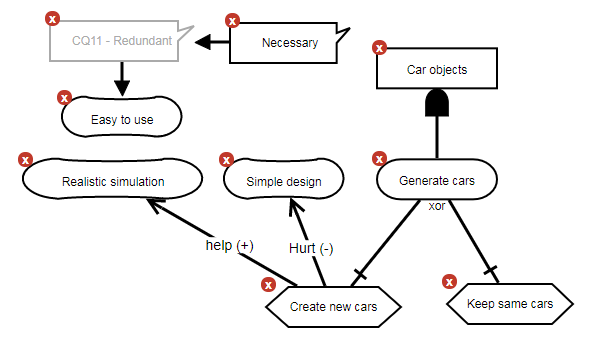
\includegraphics[scale=0.8]{img/tool/model1a}
\caption{RationalGRL model of Figure~\ref{fig:example-small3} modeled in the RationalGRL tool}
\label{fig:tool:figfrompaper}
\end{figure}

\begin{figure}[ht]
\centering
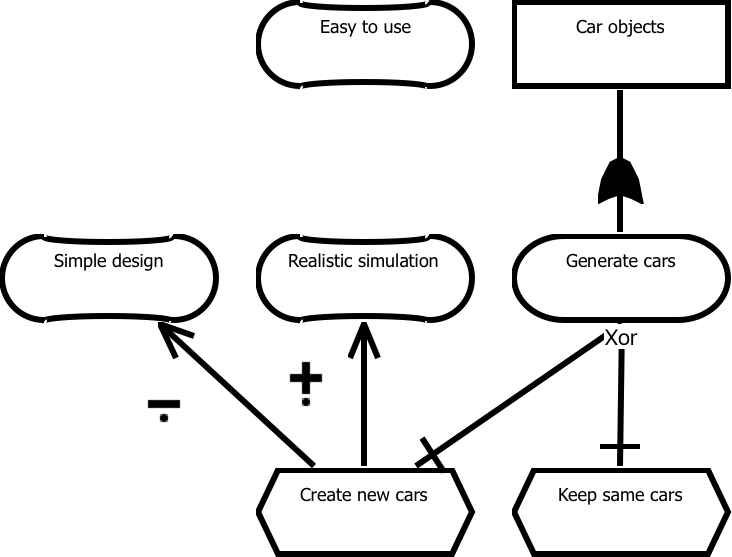
\includegraphics[scale=0.3]{img/tool/GRLmodel1a}
\caption{Exporting the model Figure~\ref{fig:tool:figfrompaper} to GRL gives the the above model in jUCMNAv}
\label{fig:tool:figfrompaper1}
\end{figure}

\begin{figure}[ht]
\centering
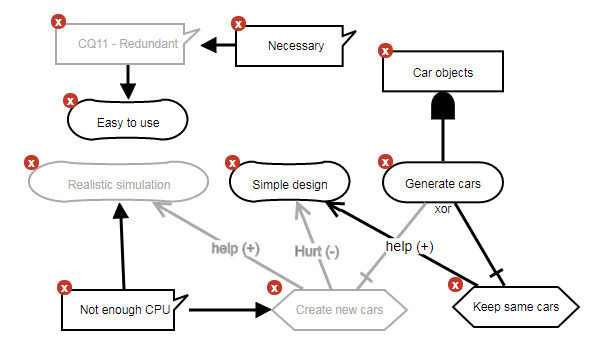
\includegraphics[scale=0.8]{img/tool/model2}
\caption{Adding an argument that attacks multiple GRL elements to Figure~\ref{fig:tool:figfrompaper}}
\label{fig:tool:multipleattack}
\end{figure}

\begin{figure}[ht]
\centering
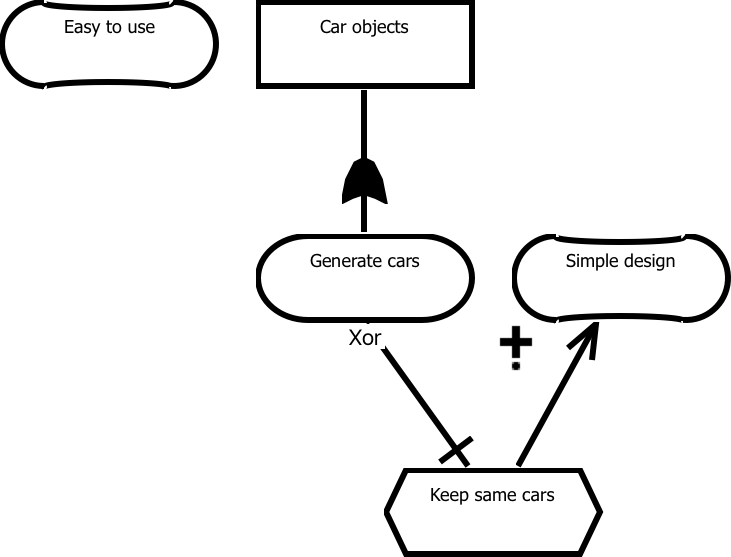
\includegraphics[scale=0.3]{img/tool/GRLmodel1b}
\caption{Exporting the model Figure~\ref{fig:tool:multipleattack} to GRL gives the the above model in jUCMNAv}
\label{fig:tool:multipleattack1}
\end{figure}
\newpage
$\ $\\
\newpage
\section{Modeling Task - Traffic Controller}
\label{sect:survey}

A group of three engineers (E1, E2, and E3) is tasked with designing a traffic flow simulation program. They receive a task specification, focusing on how the simulator will handle the generation of cars in the simulation. Below is an excerpt discussing the early requirements of the system. You are asked to model this discussion in as much detail as possible in the RationalGRL tool (http://www.rationalgrl.com), using all the tools RationalGRL puts at your disposal (GRL elements, critical questions, arguments). 

As the RationalGRL prototype does not yet have a save functionality, please save a screenshot of your final model.\\

\begin{tabular}{|p{10mm}|p{140mm}|}
\hline
\textbf{Person} & \textbf{Transcript}\\
\hline
E1 & Let's start by adding the actor "Traffic Simulator". Do you think we need to add more actors?\\
\hline
E2 & I don't think so. Let's start with the softgoals and derive the main goals and tasks from that.\\
\hline
E3 & The task description states that the simulator should be easy to use.\\
\hline
E2 & I'm not sure that we should include that. It seems to me this is redundant since any UI should be easy to use.\\
\hline
E1 & No I disagree, for some UI's it is more important than others, and the fact that they mention it explicitly in the task description means we should probably add it anyway.\\
\hline
E3 &I agree, let's keep it in, it seems necessary.\\
\hline
E1 & Ok so we have one softgoal 'easy to use'. Anything else?\\
\hline
E2 & Here it say the simulation should be realistic, and the design should be simple. I guess those are two softgoals as well.\\
\hline
E3 & Ok sounds good. So one goal of the simulation is to Generate cars. Shall we just add that as a goal?\\
\hline
E1 & Yes let's do that.\\
\hline
E2 & I think we then have two main tasks for that goal: The simulator should be able to create new cars in the simulation, and it should be able to wrap the cars when they go out of the screen.\\
\hline
E3 & So Generate cars AND-decomposes into those two tasks?\\
\hline
E1 & I don't think so actually. I think it is a XOR-decomposition. The simulation either creates new cars or wrap them when they are being reused.\\
\hline
E2 & Hmm makes sense. But then I think we should rename Wrap cars to Keep same cars.\\
\hline
E3 & Yes that is better, then Create new cars and Keep same cars are the two alternatives for the goal Generate cars.\\
\hline
E1 & Hmm what do you think about the contribution links? Should we add any?\\
\hline
E2 & Well I think if we create new cars, the simulation will be more realistic because it becomes less static. At the same time it will probably make the design less simple.\\
\hline
E3 & Yes so create new cars contributes positively to the realistic design, and negatively to simple design?\\
\hline
E2 & Hmm now I think about it, actually I think think creating new cars doesn't have much effect on the realism of the simulation.I don't think the user will notice the difference.\\
\hline
E1 & Why not? If you create new cars it changes the flow of the traffic, so I think the user will definitely notice this.\\
\hline
E2 & Okay well, ok maybe. Yes I think you are right. Let's keep the contribution link in then.\\
\hline
\end{tabular}

\newpage
\section{Example RationalGRL models from the survey}
\label{sect:survey-screenshots}

\begin{figure}[ht]
\centering
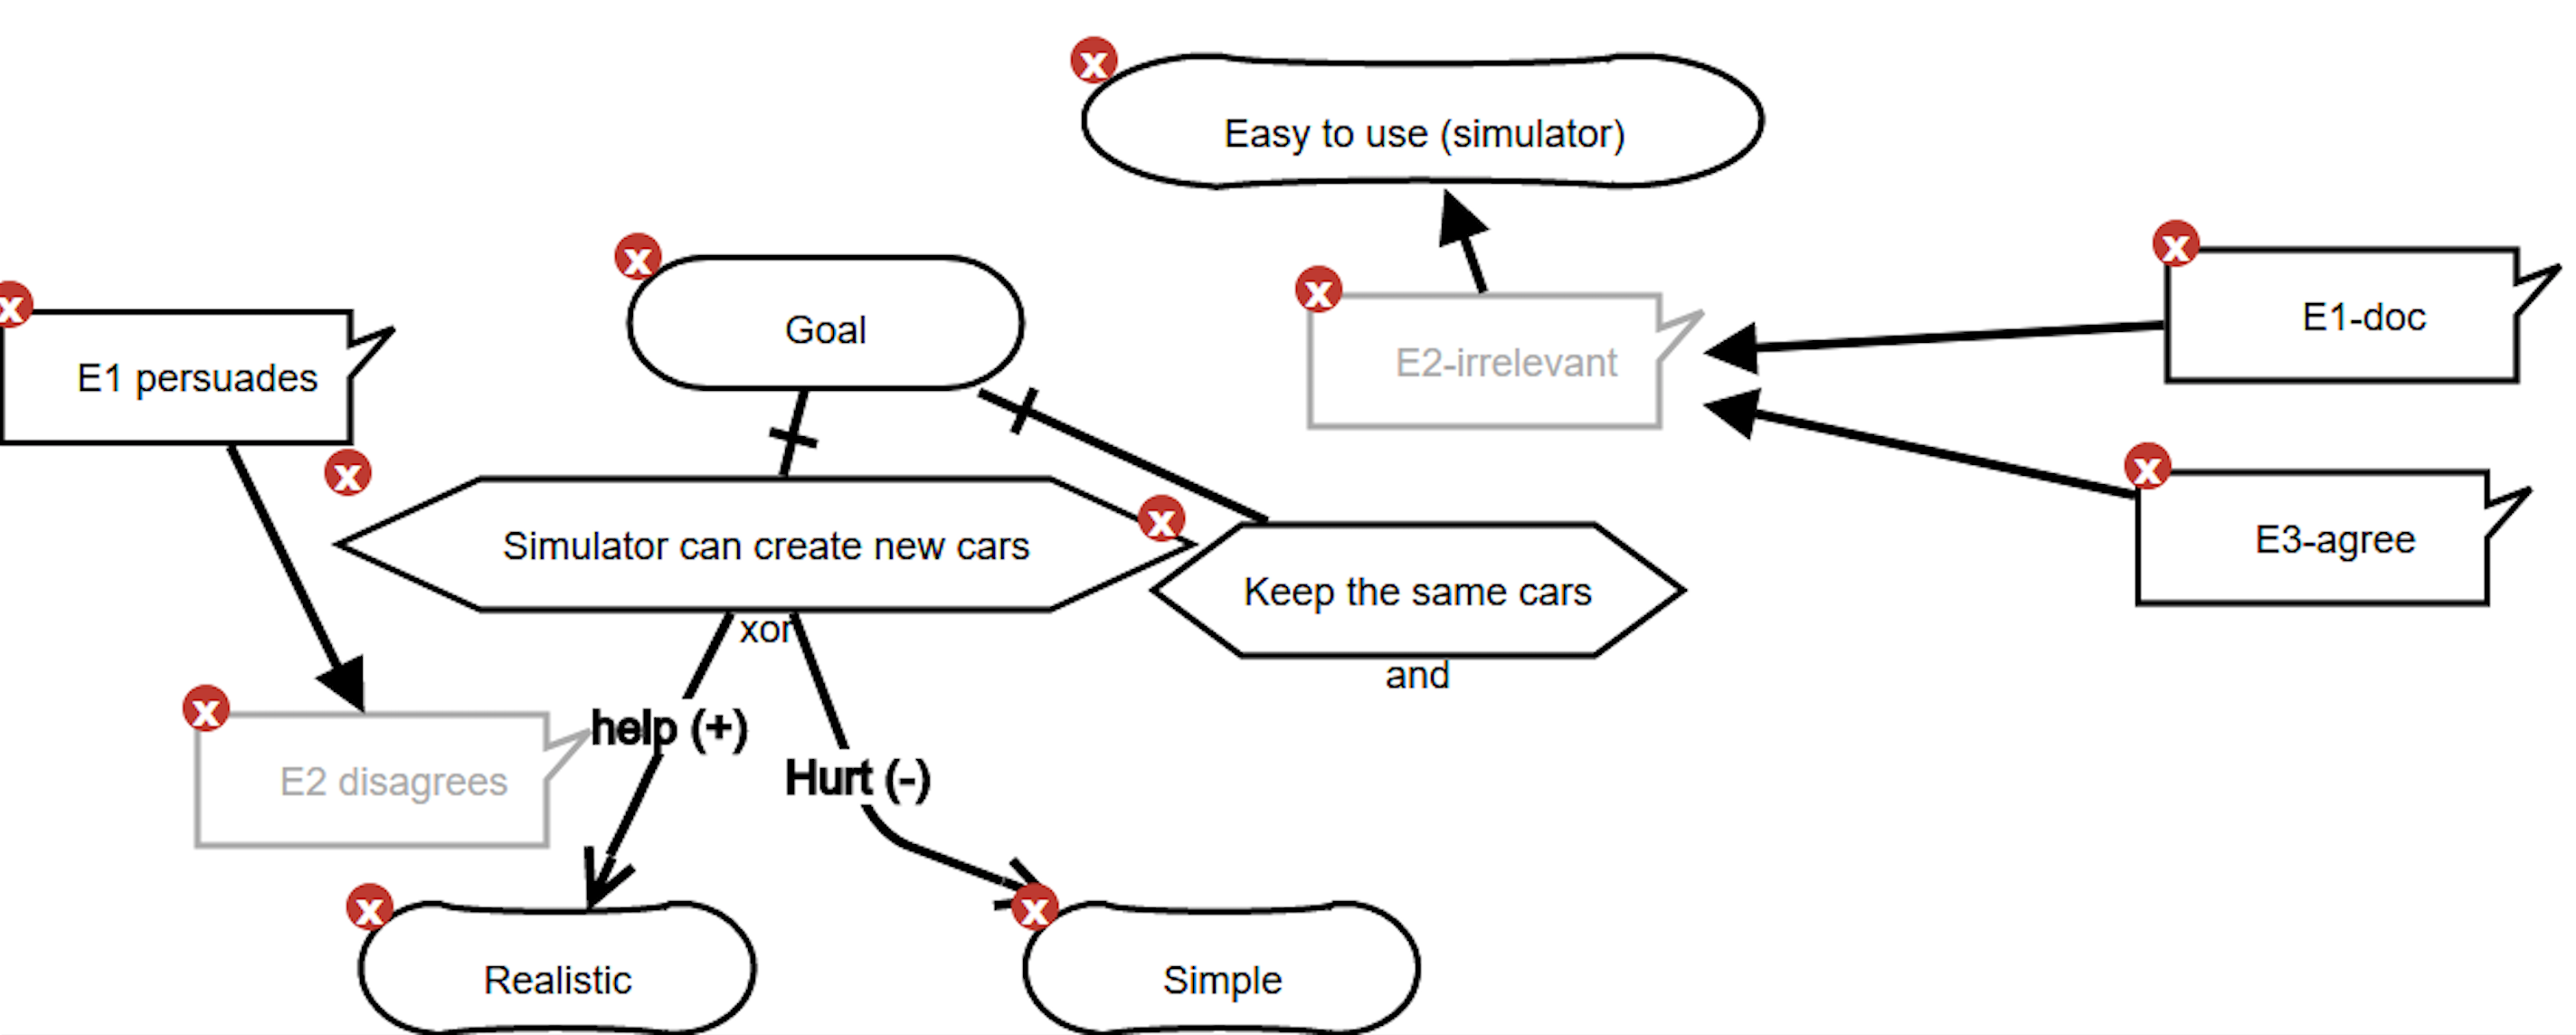
\includegraphics[scale=0.3]{img/survey/survey1}
\caption{Example model 1}
\label{fig:survey1}
\end{figure}

\begin{figure}[ht]
\centering
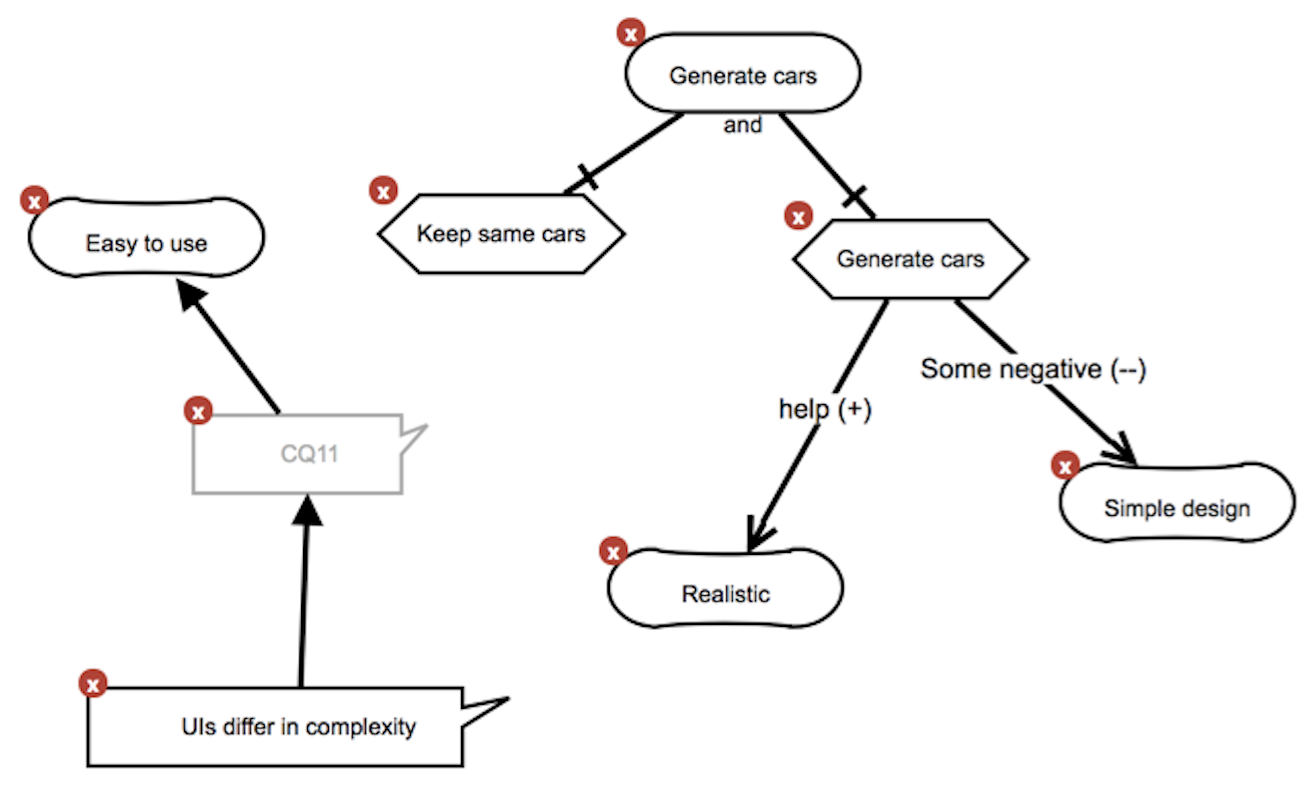
\includegraphics[scale=0.5]{img/survey/survey2}
\caption{Example model 2}
\label{fig:survey2}
\end{figure}

\begin{figure}[ht]
\centering
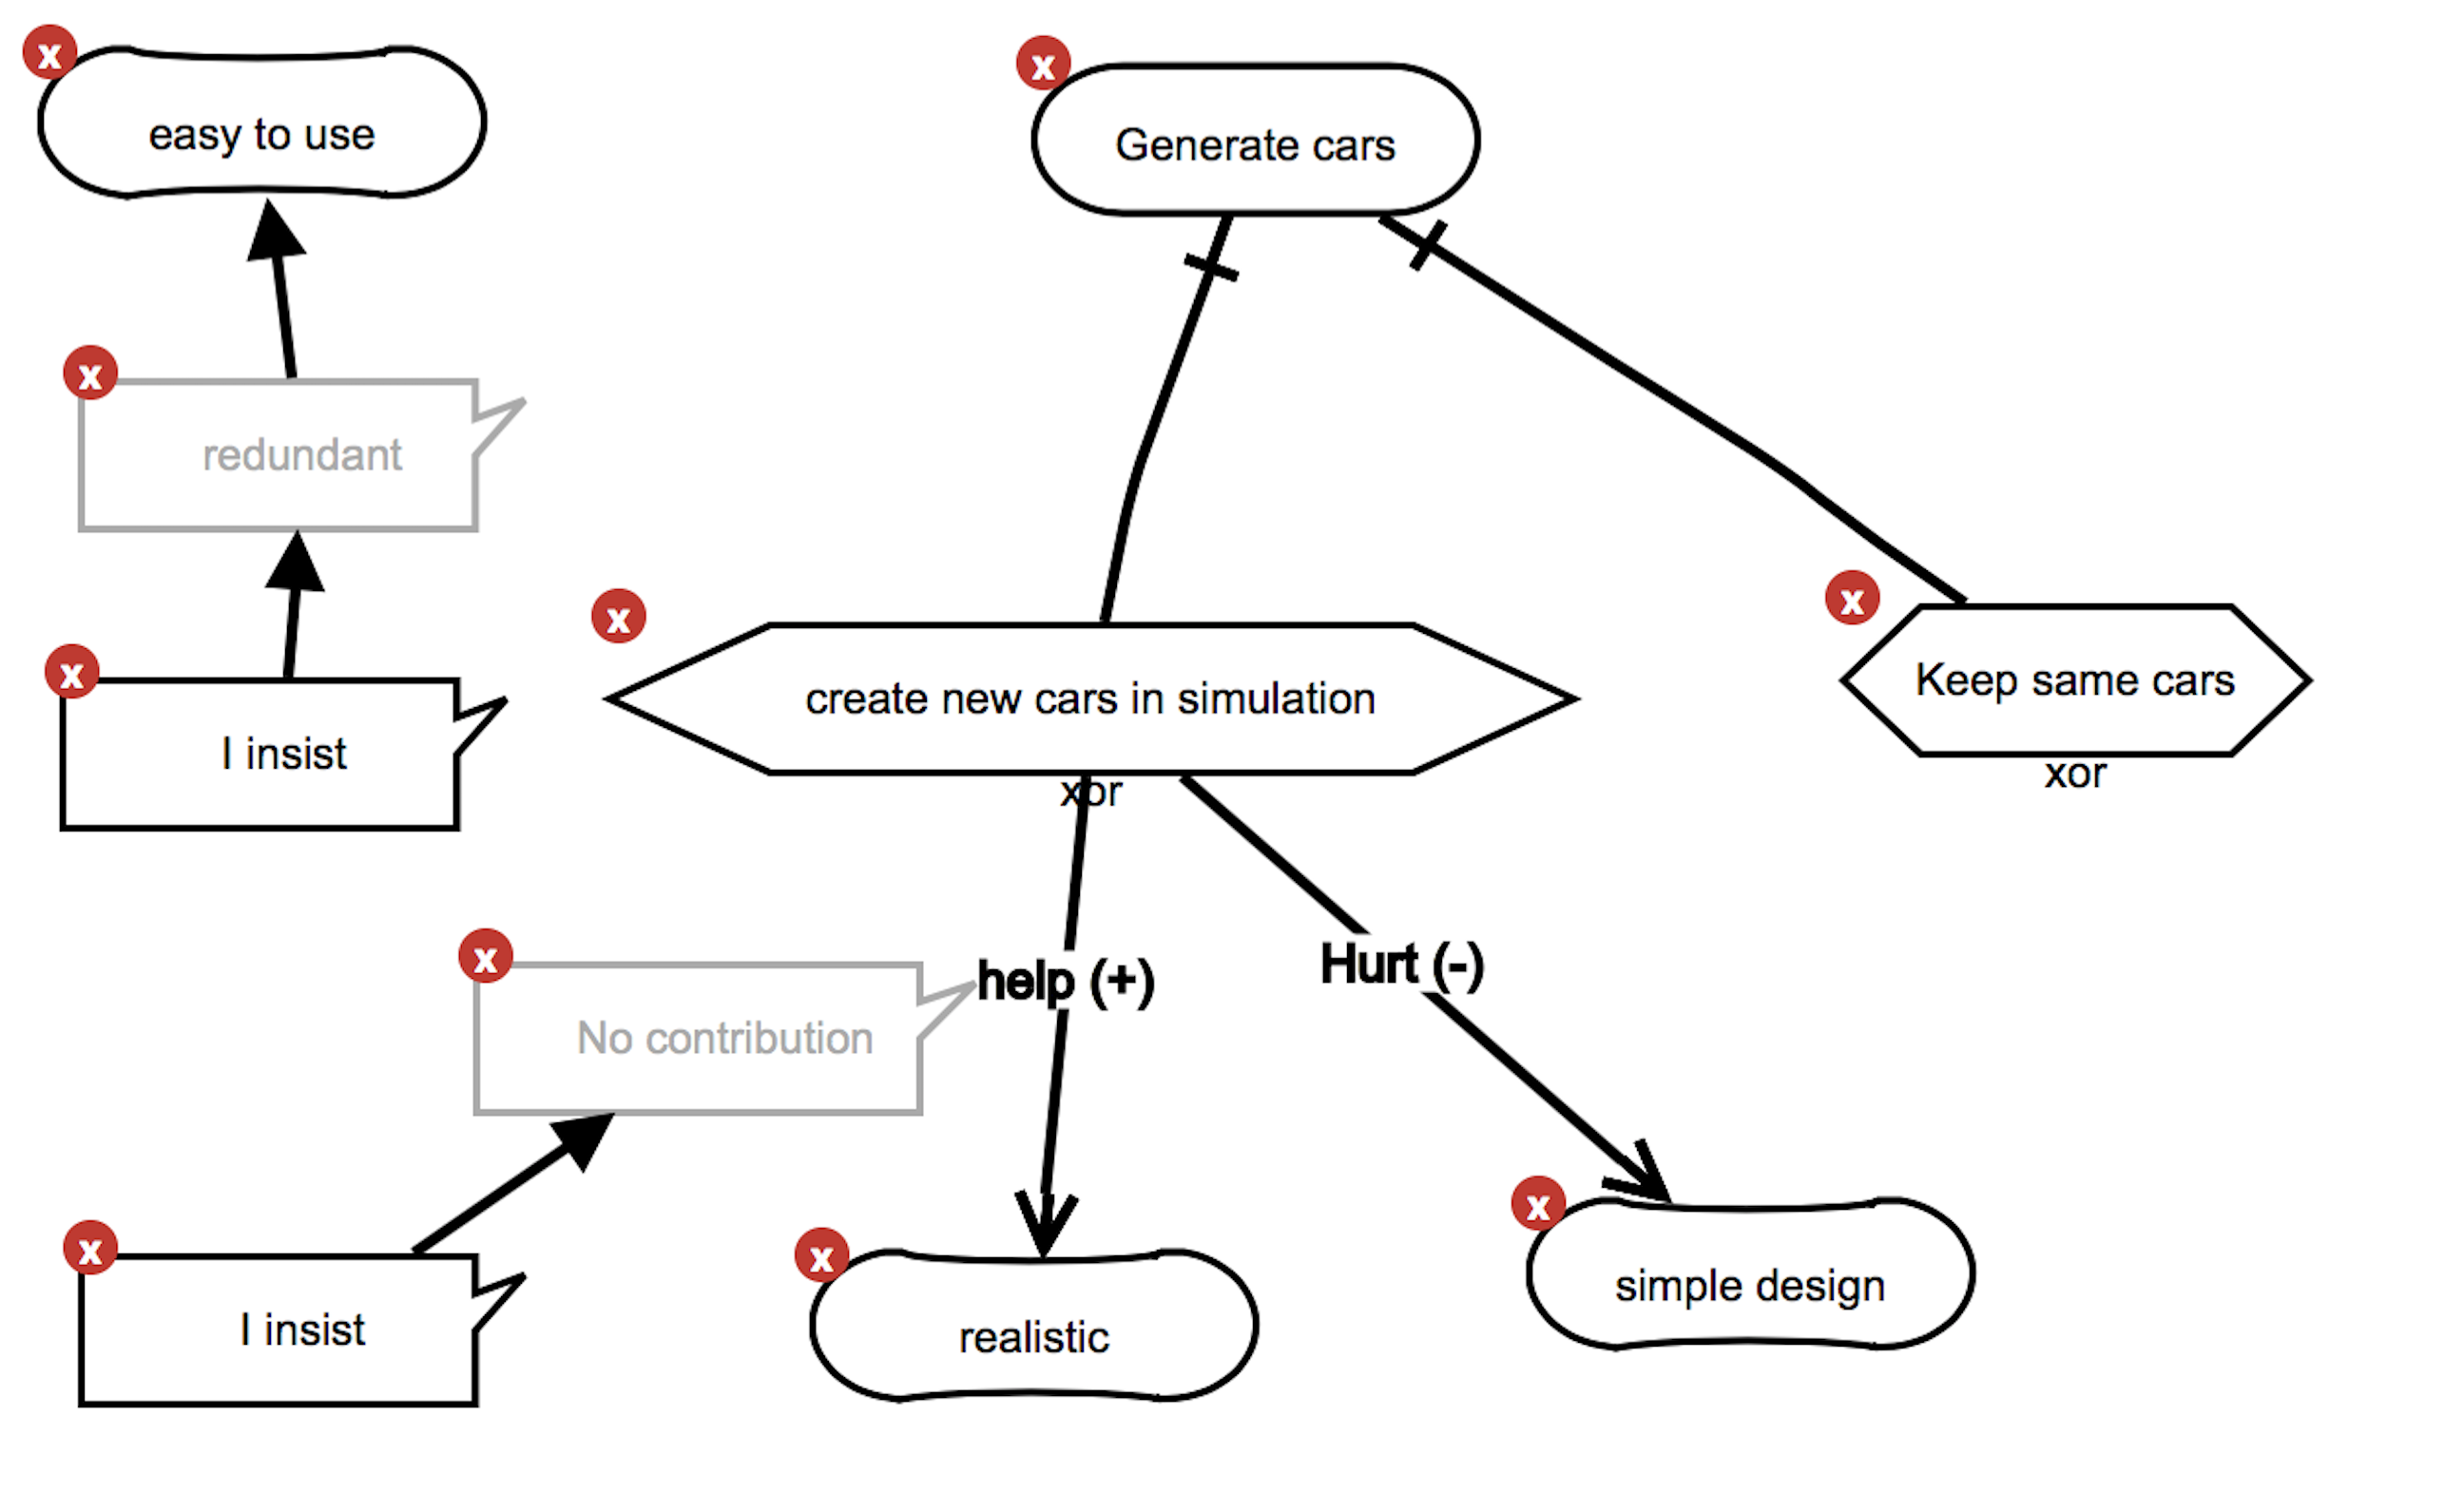
\includegraphics[scale=0.3]{img/survey/survey3}
\caption{Example model 3}
\label{fig:survey3}
\end{figure}


\end{document}